%% LaTeX2e class for student theses
%% thesis.tex
%% 
%% Karlsruhe Institute of Technology
%% Institute for Program Structures and Data Organization
%% Chair for Software Design and Quality (SDQ)
%%
%% Dr.-Ing. Erik Burger
%% burger@kit.edu
%%
%% Version 1.3, 2016-12-29

%% Available languages: english,ngerman
%% Available modes: draft,final (see README)
\documentclass[english,draft]{sdqthesis}

%% ---------------------------------
%% | Information about the thesis  |
%% ---------------------------------

%% Name of the author
\author{B.Sc. Philipp Weimann}

%% Title (and possibly subtitle) of the thesis
\title{Automated Cloud-to-Cloud migration\\
of distributed software systems\\
for privacy compliance}

%% Type of the thesis 
\thesistype{Master's Thesis}

%% Change the institute here, ``IPD'' is default
% \myinstitute{Institute for \dots}

%% You can put a logo in the ``logos'' directory and include it here
%% instead of the SDQ logo
% \grouplogo{myfile}
%% Alternatively, you can disable the group logo
% \nogrouplogo

%% The reviewers are the professors that grade your thesis
\reviewerone{Prof. Dr. Ralf H. Reussner}
\reviewertwo{Jun.-Prof. Dr.-Ing. Anne Koziolek}

%% The advisors are PhDs or Postdocs
\advisorone{Dr. rer. nat. Robert Heinrich}
%% The second advisor can be omitted
\advisortwo{Dipl.-Inform. Kiana Rostami}

%% Please enter the start end end time of your thesis
\editingtime{01. March 2017}{31. September 2017}

\settitle

%% --------------------------------
%% | Settings for word separation |
%% --------------------------------

%% Describe separation hints here.
%% For more details, see 
%% http://en.wikibooks.org/wiki/LaTeX/Text_Formatting#Hyphenation
\hyphenation{
% me-ta-mo-del
}

%% --------------------------------
%% | Bibliography                 |
%% --------------------------------

%% Use biber instead of BibTeX, see README ,backend=biber
\usepackage[citestyle=numeric,style=numeric,backend=biber]{biblatex}
\addbibresource{thesis.bib}

%% ====================================
%% ====================================
%% ||                                ||
%% || Beginning of the main document ||
%% ||                                ||
%% ====================================
%% ====================================
\begin{document}

%% Set PDF metadata
\setpdf

%% Set the title
\maketitle

%% The Preamble begins here
\frontmatter

%% LaTeX2e class for student theses: Declaration of independent work
%% sections/declaration.tex
%% 
%% Karlsruhe Institute of Technology
%% Institute for Program Structures and Data Organization
%% Chair for Software Design and Quality (SDQ)
%%
%% Dr.-Ing. Erik Burger
%% burger@kit.edu
%%
%% Version 1.3, 2016-12-29

\thispagestyle{empty}
\null\vfill
\noindent\hbox to \textwidth{\hrulefill} 
\iflanguage{english}{I declare that I have developed and written the enclosed
thesis completely by myself, and have not used sources or means without
declaration in the text.}%
{Ich versichere wahrheitsgemäß, die Arbeit
selbstständig angefertigt, alle benutzten Hilfsmittel vollständig und genau
angegeben und alles kenntlich gemacht zu haben, was aus Arbeiten anderer
unverändert oder mit Änderungen entnommen wurde.}
 
 
%% ---------------------------------------------
%% | Replace PLACE and DATE with actual values |
%% ---------------------------------------------
\textbf{PLACE, DATE}
\todo{Please replace with actual values}
\vspace{1.5cm}
 
\dotfill\hspace*{8.0cm}\\
\hspace*{2cm}(\theauthor) 
\cleardoublepage

\setcounter{page}{1}
\pagenumbering{roman}

%% ----------------
%% |   Abstract   |
%% ----------------

%% For theses written in English, an abstract both in English
%% and German is mandatory.
%%
%% For theses written in German, a German abstract is sufficient.
%%
%% The text is included from the following files:
%% - sections/abstract

\includeabstract

%% ------------------------
%% |   Table of Contents  |
%% ------------------------
\tableofcontents

\listoffigures
\listoftables

%% -----------------
%% |   Main part   |
%% -----------------

\mainmatter

%% LaTeX2e class for student theses
%% sections/content.tex
%% 
%% Karlsruhe Institute of Technology
%% Institute for Program Structures and Data Organization
%% Chair for Software Design and Quality (SDQ)
%%
%% Dr.-Ing. Erik Burger
%% burger@kit.edu
%%
%% Version 1.3, 2016-12-29

\chapter{Introduction}
\label{ch:Introduction}


\section{Motivation}
\label{sec:Introduction:motivation}

Over the last years, cloud computing has become more and more popular. This is a result of its business advantages, the continuing usage simplification and the abundance of own data centres. Netflix, for example, closed all its owned data centre in 2015 and moved completely to Amazons AWS\cite{DavidChernicoff.2015}. As a result of this trend, the expected revenue in 2016 is about 200 Billion \$\cite{statista.com.2016}. The high degree of elasticity, automation, self-service, flexibility in payment and, as a result, lower cost are only some of the many advantageous points of cloud computing.\cite{Binz.2014}

However, many – especially European - companies fear dependencies, loss of data control, industrial espionage or privacy law violations. Precautionary measures like encryption or data splitting - among data centres - is not enough to prevent a public relations disaster, due to complex EU Data Protective Regulations\cite{personaldata.2011} or the US HIPAA act\cite{OfficeforCivilRights.20130726}. To tell the whole truth, the complexity, the hidden services usages and the therefore resulting unawareness of many EU citizens (and law enforcement institutes) makes it very unlikely for current law violators to face any consequences. Nevertheless, citizens start to be more aware and the law enforcements point of attention tends to change quickly, like the Max Schrems' "Facebook Process" showed\cite{JuliaBahr.20150923}. Further, in 2018 the "reform of EU data protection rules" will come into effect, which states severe punishments for privacy violations\cite{personaldata.2011}. As a result, in the future entrepreneurs, companies and institutions need to be more aware of privacy compliance to prevent major monetary and reputation losses. 

The EU General Data Protection Regulations sets the legal boundaries for European companies. It defines multiple regulations about data handling, data trading, personal advertising and more. One rule sets the boundaries for personal data processing and saving. It states for example, that the processing of personal data is only allowed in data centres inside the EU or certain certified countries with equivalent privacy laws. As a result, software systems require a pre-deployment law compliance checking, considering especially the hosts geo-locations. The problem comes to a head with the ease of migration of whole cloud services during runtime with next to no downtime. With this in mind a potential privacy violation could occur even after the initial deployment was law compliant. This requires a non-stop observation of the applications geo-location and automatic, law compliant redeployment onto other cloud providers.


\section{Problems}
\label{sec:Introduction:problems}

To create such a privacy aware system adaptor, a couple of non-trivial problems need to be solved. The major ones will be outlined shortly, categorized after the MAPE-K feedback loop:

\begin{itemize}
	\setlength\itemsep{0em}
	\item \textbf{Monitoring}\newline
	Acquiring and transforming geo-location information onto an architecture description language
	\item \textbf{Analysing}\newline
	Privacy compliance analysis on a software architecture basis
	\item \textbf{Planning}\newline
	Computation of constraint and privacy compliant redeployments
	\item \textbf{Executing}\newline
	Technology independent, dynamic adaptation routine computation, execution and evaluation
\end{itemize}

%Transformation for geo-location into ADL
%Privacy analysis on architecture lvl
%Privacy compliant system deployment calculation
%System adaptation calculation
%System adaptation execution

%simple & efficient privacy concept for component based architecture
%what information are required?
%
%
%automatic migration with evaluation


\section{Goals and Research Questions}
\label{sec:Introduction:goals}

This thesis' goal is to contribute a piece of software, that ensures continues privacy compliance, modelled after the MAPE-K feedback loop. Wrapped into this pipeline are several interesting research questions:

\begin{itemize}
	\setlength\itemsep{0em}
	\item \textbf{Monitor}: How can information, required for privacy violation detection, be monitored? How can we transform this information onto our architecture model?
	\item \textbf{Analyse}: How to analyse the model for privacy violation detection? And how good does this analysis scale?
	\item \textbf{Plan}: How can the runtime model and analysis results be used to reacquire policy compliance?
	\item \textbf{Execute}: How can the plan automatically be executed and policy compliance established? How much human interaction is necessary?
\end{itemize}

\todo{Individual goals for the MAPE loop? Feels redundant, doesn't it?}


\section{Outline}

The remainder of this thesis is structured as following: The thesis continues by introducing the foundations (\autoref{ch:Foundations}) and the related work (\autoref{ch:RelatedWork}) of this thesis. The main part starts with the privacy concept (\autoref{ch:PrivacyConcept}), leading into the system overview (\autoref{ch:Overview}), followed by the big conceptual work packages: Palladio modification (\autoref{ch:pcmExtension}), iObserve extension (\autoref{ch:iObserve}), privacy analysis (\autoref{ch:PrivacyAnalysis}), PerOpteryx extension (\autoref{ch:PerOpt}) and the system adaptation (\autoref{ch:SysAdap}). The thesis closes with the evaluation (\autoref{ch:Evaluation}) and finally the conclusion (\autoref{ch:Conclusion}).



%%%%%%%%%%%%%%%%%%%%%%%%%%%%%%%%%%%%%%%%%%%%%%%%%%%%%%%%%%%%%%%%%%%%%%
\chapter{Foundations}
\label{ch:Foundations}

In this chapter we introduce applications and principles, this thesis is based on. This introduction aims for a general understanding. Some aspects my be discussed in more detail in the corresponding section of this thesis.

\section{MAPE-K loop}
\label{sec:Foundations:mape}

MAPE-K or MAPE was first introduced by IBM for automatic computing and later discussed in the context of self-adaptive systems. A MAPE system is usually a stand alone application, which is specially build for optimizing and adapting a monitored system. MAPE-K is an acronym, consisting of the first letters of the loops stages: Monitor, Analyse, Plan, Execute and Knowledgebase. These stages are sequentially ordered in a pipeline structure, each one has a well defined task:

\begin{itemize}
	\setlength\itemsep{0em}
	\item \textbf{Monitor}: Collects, aggregates, filters and correlates information about a monitored system.
	\item \textbf{Analyse}: Performs (complex) data analysis and reasoning on the monitored data. The analysis is often supported by data from the knowledgebase. If changes are required, a change request is passed to the plan function.
	\item \textbf{Plan}: Determines what kind of changes are required and develops a transformation which adapts the monitored system towards the desired state.
	\item \textbf{Execute}: Executes the transformation calculated during the planning phase.
	\item \textbf{Knowledgebase}: Additional or advanced information that are shared among all stages.
\end{itemize}

The monitored system runs independently from the MAPE application. However, the desired monitoring information are usually explicitly provided via specially designed APIs, intefaces or probes.


\section{Palladio Component Model}
\label{sec:Foundations:pcm}

The Palladio Component Model (short PCM) is an Architecture Description Language (ADL) for component based software, originally designed to enable software architects to run pre-implementation performance analysis. The Palladio Simulator reports on "performance bottlenecks, scalability issues, reliability threats, and allows for a subsequent optimisation." The PCM is composed of several sub-models which depend on another. Each model represents a certain aspect of a component based software:

\begin{itemize}
	\setlength\itemsep{0em}
	\item \textbf{Repository Model}: Defines Components with required and provided interfaces. Interfaces include function signatures. 
	\item \textbf{System Model}: Defines the complete software system, by connecting components defined in the repository model.
	\item \textbf{Usage Model}: Defines process workload, based on the systems interfaces.
	\item \textbf{Resource Environment Model}: Defines available host environments with its provided performance.
	\item \textbf{Allocation Model}: Defines the deployment of system components onto the provided hosts.
\end{itemize}

The separation of concern enables the system architect to manage the complexity of even bigger software systems and still gain meaningful results from the performance simulation.

Since its initial release the Palladio Component Model was adapted and used in several research fields alongside the performance prediction like automated Dataflow Analysis and Application Monitoring. Due to its explicit representation of the software architecture and flexible component-host-mapping it is perfectly suited to model distributed cloud systems. Although, PCM was not designed to be used as a runtime model, it has proven to be suited for this task due to its versatile model elements.

\section{Kieker}
\label{sec:Foundations:Kieker}

Kieker is a software system monitoring application with the goal of retrieving runtime information for performance evaluation, (self-)adaptation control and many other tasks. Kieker gains these information from the designated software by instrumenting the system with probes during pre-compilation. Each probe has designated purpose and gathers data accordingly, for example hardware utilization, stack trace or host geo-location. Kieker uses event-based probes, as well as periodic-based (heart-beat) probes.


\section{iObserve}
\label{sec:Foundations:iobserve}

iObserve is based on Kieker and therefore also a software monitoring application. However, iObserve uses the monitored information to update the systems Palladio model during execution, making it a runtime model. Further, iObserve and the extended Kieker version are deigned to support distributed cloud systems. Key features are the transformation form the gathered information onto the model update. Using the stack trace information the PCM usage model can be updated and more precise performance simulations created. 

Currently, iObserve goes as far as updating the model, representing the first stage "Monitoring" of the MAPE-K loop. iObserve uses the Teetime framework, a pipeline-filter-framework with signal based state invocation.\cite{Heinrich.2016}

\section{PerOpertyx}
\label{sec:Foundations:peropteryx}

"PerOpteryx is an optimization framework to improve component-based software architecture". Optimization uses model-based quality prediction techniques. Starting from an input model, the framework generates multiple pareto optimal alternative deployments, based on given simulation and alternation algorithms. PerOpteryx make architecture adjustments via multiple approaches like alternating components multiplicity, runtime parameters or changing component allocations. The Pareto optimality models are calculated through multiple iterations via a series of stages. Initially a variance of candidates is created though evolutionary algorithm and random generation/mutation. In the next step, the candidates get analysed for the desired quality marks and ranked accordingly. The iteration concludes with the elimination of poorly performing candidates. The framework terminates with a cost rating of all Pareto optimum candidates.


%%%%%%%%%%%%%%%%%%%%%%%%%%%%%%%%%%%%%%%%%%%%%%%%%%%%%%%%%%%%%%%%%%%%%%
\chapter{Related Work}
\label{ch:RelatedWork}


\section{Application Monitoring}
\label{sec:RelatedWork:appl_mon}

The monitoring of software systems is common task in many research fields. Automated data-flow analysis, software profiling and hardware utilization are only a small selection of groups, using this term. In the following, we use application monitoring in the sense of online extraction of runtime data form a (distributed cloud) application for architecture optimization.

R-PRIS (\autoref{sec:RelatedWork:privacyanalysis}) and Kieker are application monitoring frameworks. While iObserve uses Kieker to extract the desired information, R-PRIS is independent from other programs. Neither of them uses a meaningful architecture description language (ADL) to process and store the gathered information. iObserve however gathers the transmitted data, processes them and stores them into a PCM model, enabling all sorts of PCM-based applications to use the gathered information.
\todo{gather more details \& Refs} 


\section{Privacy Analysis}
\label{sec:RelatedWork:privacyanalysis}

R-PRIS is a monitoring and analysing tool for distributed cloud systems. Like iObserve, R-PRIS updates a runtime model by monitoring the cloud systems. During the analysis phase the model is checked for (potential) privacy violations.

R-PRIS combines push-based heartbeat monitoring with event processing, and graph grammars for efficiently updating those models.\cite{Schmieders.}
\todo{Add more details?}

R-PRIS uses a formal specification for geo-location policies. These consists of data classification $S$, data content types $T$ and geo-locations $L$. Every specified policy $p = (S, T, L)$ is forbidden.
During privacy analysis R-PRIS checks whether a privacy protected information can be accessed from an non-privacy compliant location. This can be transformed into an st-connectivity problem, a standard problem in graph theory and analysis. Based on the runtime model (\autoref{fig:rpris_model}) - with its meta-model (\autoref{fig:rpris_metamodel}) - R-PRIS performs a reachability check.\cite{Schmieders.2015} 

\begin{figure}[h]
	\centering
	\begin{minipage}[b]{0.48\textwidth}		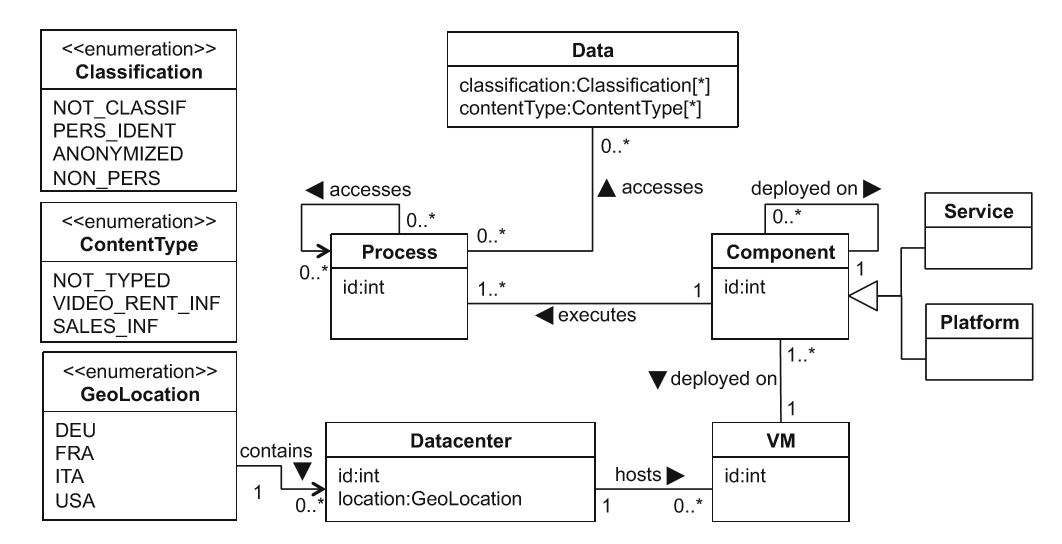
\includegraphics[width=\textwidth]{pictures/rpris_metamodel.jpg}
		\caption{R-PRIS meta-model}
		\label{fig:rpris_metamodel}
	\end{minipage}
	\begin{minipage}[b]{0.48\textwidth}
		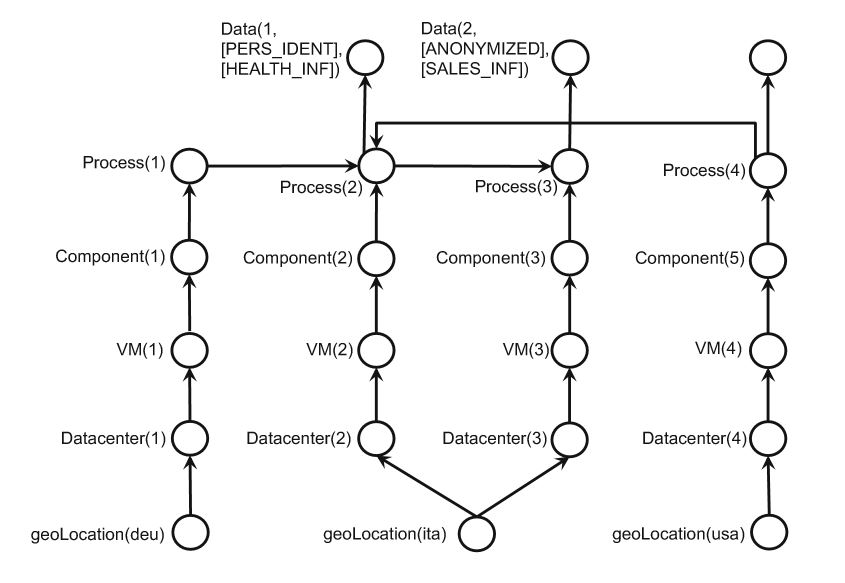
\includegraphics[width=\textwidth]{pictures/rpris_model.jpg}
		\caption{R-PRIS runtime model}
		\label{fig:rpris_model}
	\end{minipage}
\end{figure}

In terms of software, R-PRIS searches for communication paths in the distributed system, which can potentially transmit personal data to a non-privacy compliant geo-location. In order to detect these communication paths a policy $p$ must be specified, representing exactly this case, which however doesn't necessarily communicate private data. As a result, a lot of policies have to be specified, which as a result prohibits many potentially harmless communication paths.

Based on their runtime model, Schmieders et al. identified four relevant migration-cases and extracted six required informations to detect a policy violation\cite{Schmieders.2015}:

\begin{table}[h]
	\centering
	\begin{tabular}{r | l}
		\hline
		\textbf{\#} & \textbf{Required information to carry out runtime check}\\
		\hline
		R1 & Interactions of two components\\
		R2 & Access of components to locally stored files\\
		R3 & Meta-information of stored or processed data\\
		R4 & Information on component deployments on physical resources \\
		R5 & Geo-location information of physical resources\\
		R6 & Explicit or implicit information on transitive data transfers\\
		\hline
	\end{tabular}
	\caption{R-PRIS information for runtime privacy checks \cite{Schmieders.2015}}
	\label{tab:rpris_information}
\end{table}


\section{Data-flow Analysis \& Rights Management}
\label{sec:RelatedWork:dataflow}

(Access) Rights Management, like the Bell-LaPadula Model or Role-based access control, are fundamentals in our modern information society. These systems restrict or allow access on certain entities with the intention of information protection. The fundamentals are well researched, so research currently is focused on resource and time efficient rights management in large scale systems like companies, as well as automated rights management on small, mobile devices \cite{Dinger.2008}.

Data-flow Analysis is a hot research topic due to the omnipresence of cloud services and mobile devices with rich data sources. Applications like \textit{JOANA} \cite{Snelting.2014}, \textit{TaintDroid} \cite{Enck.2014}, \textit{Privacy Oracle}  \cite{Jung.2008} or \textit{automated privacy instrumentation} \cite{Suh.2004} are only some of many applications and approaches around data-tracking, data-flow analysis and leak detection. However, nearly all of these approaches are using actual code or information rich models.

For our purposes we need automated data-flow analysis on architecture level, to determine if a system violates privacy regulations. This research is still in its fledgling stages and therefore not suited for applications with our designated level of complexity.


\section{Privacy Analysis}
\label{sec:RelatedWork:privacy_check}

Most research in this field focuses on prevention of policy violation. “However, changes of data geo-locations imposed by migration or replication of the component storing the data are not considered. Data transfers between the client services and further services are not covered. Transitive data transfers that may lead to policy violations thus remain undetected.”\cite{Schmieders.2015}

As mentioned in \autoref{sec:RelatedWork:privacyanalysis}, R-PRIS is searching for potential access violations in the application model, by using a st-connectivity analysis.\cite{Schmieders.2015}\cite{Schmieders.} This approach is overestimating the privacy aspects by not including which kind of data are actually communicated between components and geo-locations. This makes it impractical for many business applications due to likelihood of allowing only save-considered components deployment.



\section{Automated Model Optimization \& Modification}
\label{sec:RelatedWork:auto_model_opt}

The research field of model analysis based performance optimizer can be roughly divided into two sections. First, the rule-based approaches, which apply a predefined rule, based on the detected problem, onto the system model. Second, metaheuristic-based approaches, which use a generic framework and evolutionary algorithms for multiple arbitrary quality criteria.\cite{Martens.2010}

PerOpteryx (\autoref{sec:Foundations:peropteryx}) is a metaheuristic-based approach. However, PerOpteryx does not consider a hosts geo-location during its optimization process. This can be changed by adding an allocation constraint, preventing privacy violating deployments. 



\section{Automated Cloud Migration}
\label{sec:RelatedWork:cloud_migration}

Since the start of cloud computing there has been plenty of research on how to migrate regular on premise applications and software into the cloud. Either software is cloud-enabled in the most automatic fashion possible or the software is cloud-native, meaning specially developed or redesigned, by developers, for running inside the cloud. While there has been good progress semi-automatically cloud-enabled software, the field of migrating cloud applications form one cloud provider to another is just beginning. One of the main issues is resulting in provider individual Cloud-APIs. Current, state of the art is the "Docker" or container-technology, which wraps the application like a VM and is suitable for many cloud provider. Nevertheless, many cloud provider offer special purpose solutions, where a docker solution is not viable. The technology side of cloud to cloud migration will be left out in this thesis. \cite{Jambunathan.February2016}\cite{Binz.2014} 
%% LaTeX2e class for student theses
%% sections/content.tex
%% 
%% Karlsruhe Institute of Technology
%% Institute for Program Structures and Data Organization
%% Chair for Software Design and Quality (SDQ)
%%
%% Dr.-Ing. Erik Burger
%% burger@kit.edu
%%
%% Version 1.3, 2016-12-29

\chapter{Privacy Concept}
\label{ch:PrivacyConcept}

Many say: Data is the new oil and the most valuable resource there is. This shows how important the control of our personal data is. To achieve this, many players have to fulfill their obligations. On the one hand, the personal awareness of every user himself to only communicate the required and necessary information. On the other hand, the data handling institutes duty to guarantee legal compliance to laws like the EU’s general data protective regulations. While one can't act for the individual, we can provide tools and rules for institutions to help with legal compliance.

\section{General Concept}
\label{sec:PrivacyConcept:general}

The EU General Data Protective Regulations clearly states, that data of EU citizens have to be saved and processed within EU countries \cite{personaldata.2011}. Only a view countries with equal data protective laws are excepted from this constraint. As a consequence, one needs a simple data-flow analysis (\autoref{sec:RelatedWork:dataflow}) to know the data distribution in our software system. To put it straight, one needs to know, what kind of data are available on which server. This task got especially important, since distributed cloud systems are reality and data saved on "on premise" servers are becoming increasingly rare.

As mentioned in \autoref{sec:RelatedWork:dataflow}, the automated data-flow analysis on architecture level is still in its early stages and therefore not suited for practice. As a compromise we decided on manual data tagging. To ease the data tagging and analysis process, we decided to use the common well defined categories \cite{Schmieders.2015}:
%A growing and continuous research field is exploring and developing approaches for automated data-flow analysis. However, these are still very limited and are therefore not yet suited for practice (see \autoref{sec:RelatedWork:dataflow}). Due to these limitations, we need manual annotation of components.

\begin{itemize}
	\item \textbf{Type 0: Personal Information}: Data relates directly or indirectly to personal information. This is independent from encryption or pseudonymization. (e.g. call detail record)
	
	\item \textbf{Type 1: Personally Identifiable Information}:  Data does not contain personal information. However, by combining, fusing or analysing data sets, the personal data could be reconstructed for complete or partial personal information. (e.g. browser history without user)
	
	\item \textbf{Type 2: Anonymous Data}: Data does not contain any personal information. Even by extensive data analysis no direct or indirect personal information can be extracted. (e.g. shop inventory data)
	
	\label{sec:PrivacyConcept:dataprivacylevel}
\end{itemize}

These three categories are used, since many data do not contain any direct or indirect link onto private data, however still contain indicators onto private data. This means, they neither qualify for the type 0 category (Personal), nor for the type 2 category (Anonymous). For example an online shop wants to analyse which products usually get ordered together. The orders got anonymized by removing the customer and shipping address. Nevertheless, the time-stamp is required to get a timed evaluation factor. These data are not personal. However, combining and evaluating these with user-login-times, also non-personal data, privacy relevant data can be extracted. This also disqualifies them for Type 2, completely anonymous data \cite{Schmieders.}\cite{Schmieders.2015}.

Summarizing, a manual, categorized annotation approach to identify the system components privacy level is used. Based on this privacy level categorization, the analysis, whether a systems deployment is privacy compliant, can be performed.


\section{Deployment Constraints}
\label{sec:PrivacyConcept:deploymentrules}

How can one guarantee legal compliant distribution? As mentioned in \autoref{sec:Introduction:motivation}, personal data of EU citizens are only allowed to be processed, transferred or saved inside EU countries [...]. We argue that the following constraints, combined with correct manual annotation, are sufficient to accomplish this:

\begin{itemize}
	\label{enum:deployment_rules}
	\setlength\itemsep{0em}
	\item \textbf{Rule \#1}: Type 0 components must be deployed in a "save" geo-location.
	\item \textbf{Rule \#2}: Type 2 components can be deployed anywhere.
	\item \textbf{Rule \#3}: Type 1 components can be deployed anywhere.
	\item \textbf{Rule \#4}: Only deploy Type 1 components together in an "un-save" geo-location, if they receive their information (transitively) from the same Type 1 component.
	% Only deploy Type 1 components (x_1, x_2, ...) together in an "un-save" geo-location, if a connected set X containing at least (x_1, x_2, ...) with only type 1 or type 2 components exists, that has a maxium of one connection to a type 0 componont
\end{itemize}

\textit{Rule 1 \& 2} does not need any further explanation. \textit{Rule 3} states that Type 1 components can be deployed anywhere. This is due to the fact that Type 1 data should not contain any personal information. \textit{Rule 4} however limits this deployment. This constraint is necessary, because the combination of multiple Type 1 data streams could lead to privacy relevant information. If the data streams, however, have a common type 1 component as data source, the deployment can be considered privacy compliant.

The ideas is, when a depersonalised component (d) has a single edge to a personal component (p), and many edges to other depersonalised components (D), and the components (D) do not have any connection a personal categorized component, then they share the data passed via the connection between d and p, which can not be personal. Otherwise d would be categorized as personal. Note that data streams with type 2 components can be ignored, since - by definition - they don't get in contact with any privacy relevant data. 

We are aware, that these rules are over-approximations towards legal compliance. However, we are using a software architecture model as the only source of information. Therefore, detailed information about actual privacy symbiotic data streams are not available on this high level ob abstraction. Nevertheless, we argue, that these rules already help to identify illegal deployments and establish privacy compliant (re-)deployments.

\autoref{fig:example_depl:1}, \autoref{fig:example_depl:2} and \autoref{fig:example_depl:3} illustrate the different base scenarios applying to Rule 4. In the remainder of this section, we will elaborate their privacy compliance state by applying \autoref{enum:deployment_rules}, rule 4.

\begin{figure}[h]
	\centering
	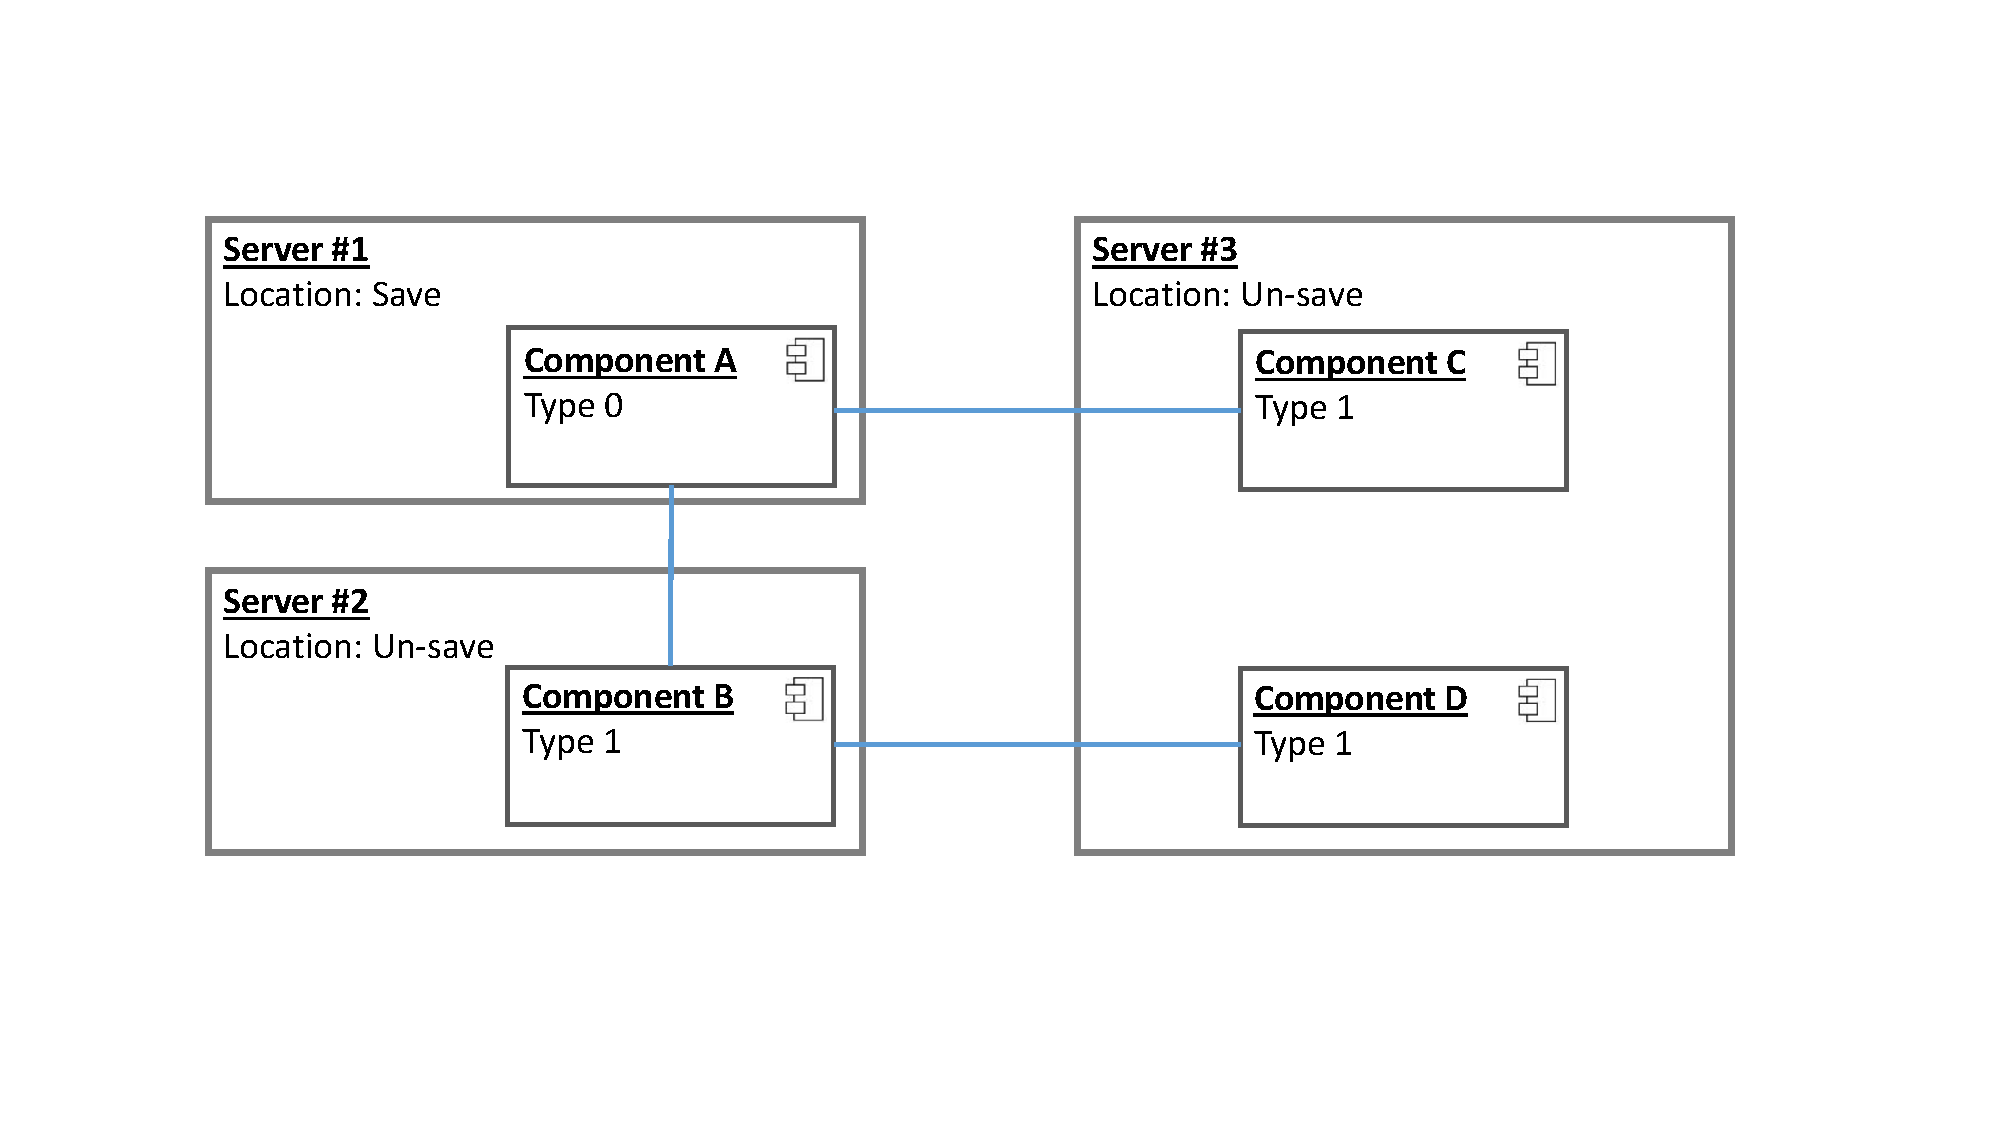
\includegraphics[trim = 35mm 45mm 40mm 30mm, clip, width=0.6\textwidth]{graphs/deployment_example_1}
	\caption{Privacy violating deployment}
	\label{fig:example_depl:1}
\end{figure}

The deployment shown in \autoref{fig:example_depl:1} is illegal. Server\#3 contains components with data streams from two different components, where one is a type 1 and one is a type 0 component. Even though A and C receives its data transitively from the same source, component A. This source is categorized as personal (type 0). Further, the data passes via different initial communication edges. As a result, \textit{Server \#3} hosts two type 1 components, which don't contain privacy relevant data by themselves. However, after combination, the data could be privacy relevant. So, this deployment is considered illegal.

\begin{figure}[h]
	\centering
	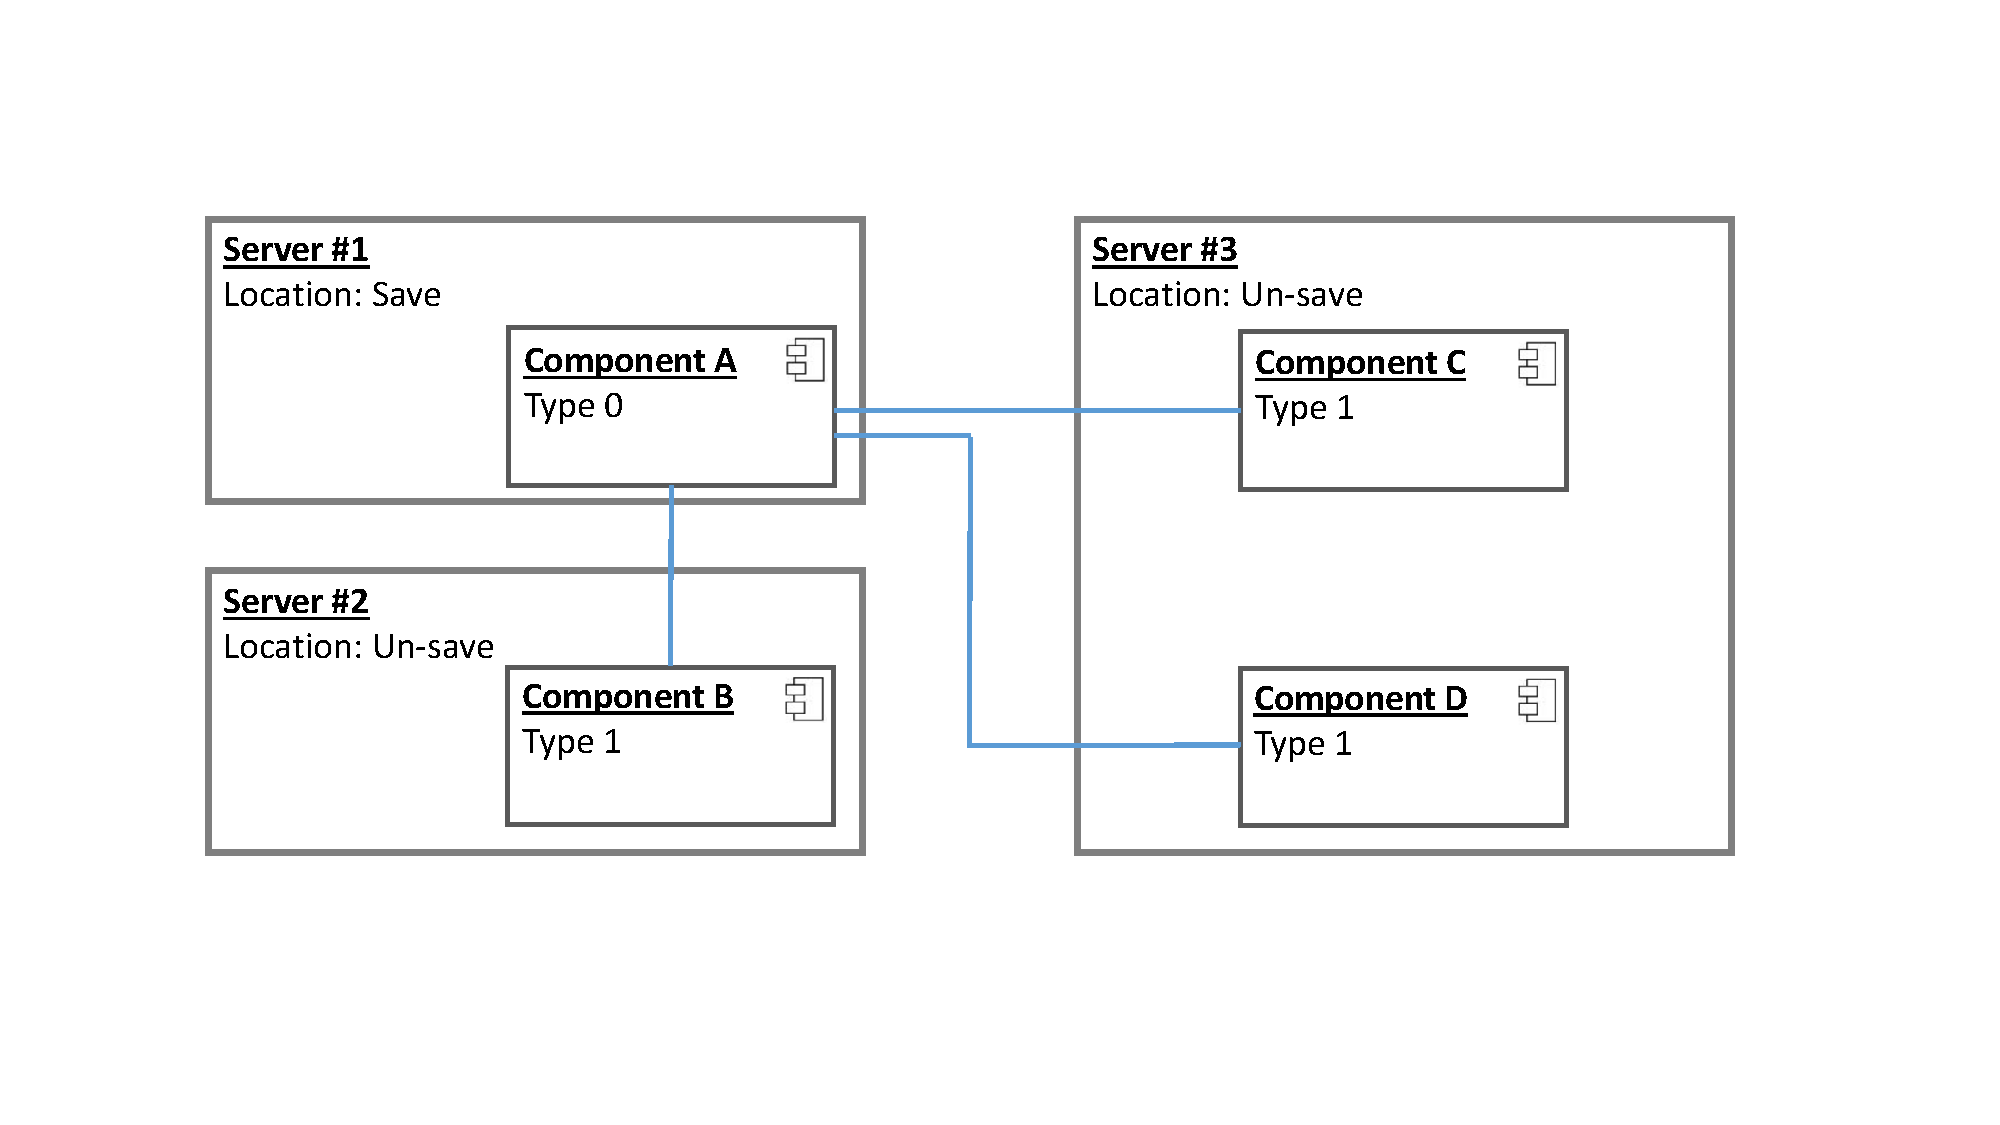
\includegraphics[trim = 35mm 45mm 40mm 30mm, clip, width=0.6\textwidth]{graphs/deployment_example_2}
	\caption{Privacy violating deployment}
	\label{fig:example_depl:2}
\end{figure}

\autoref{fig:example_depl:2} also shows an illegal considered deployment. Component C and D share the same data source, which is marked as type 0. As previously shown, the combination of data on Component C and D could lead to privacy relevant informations on \textit{Server \#3}.

\begin{figure}[h]
	\centering
	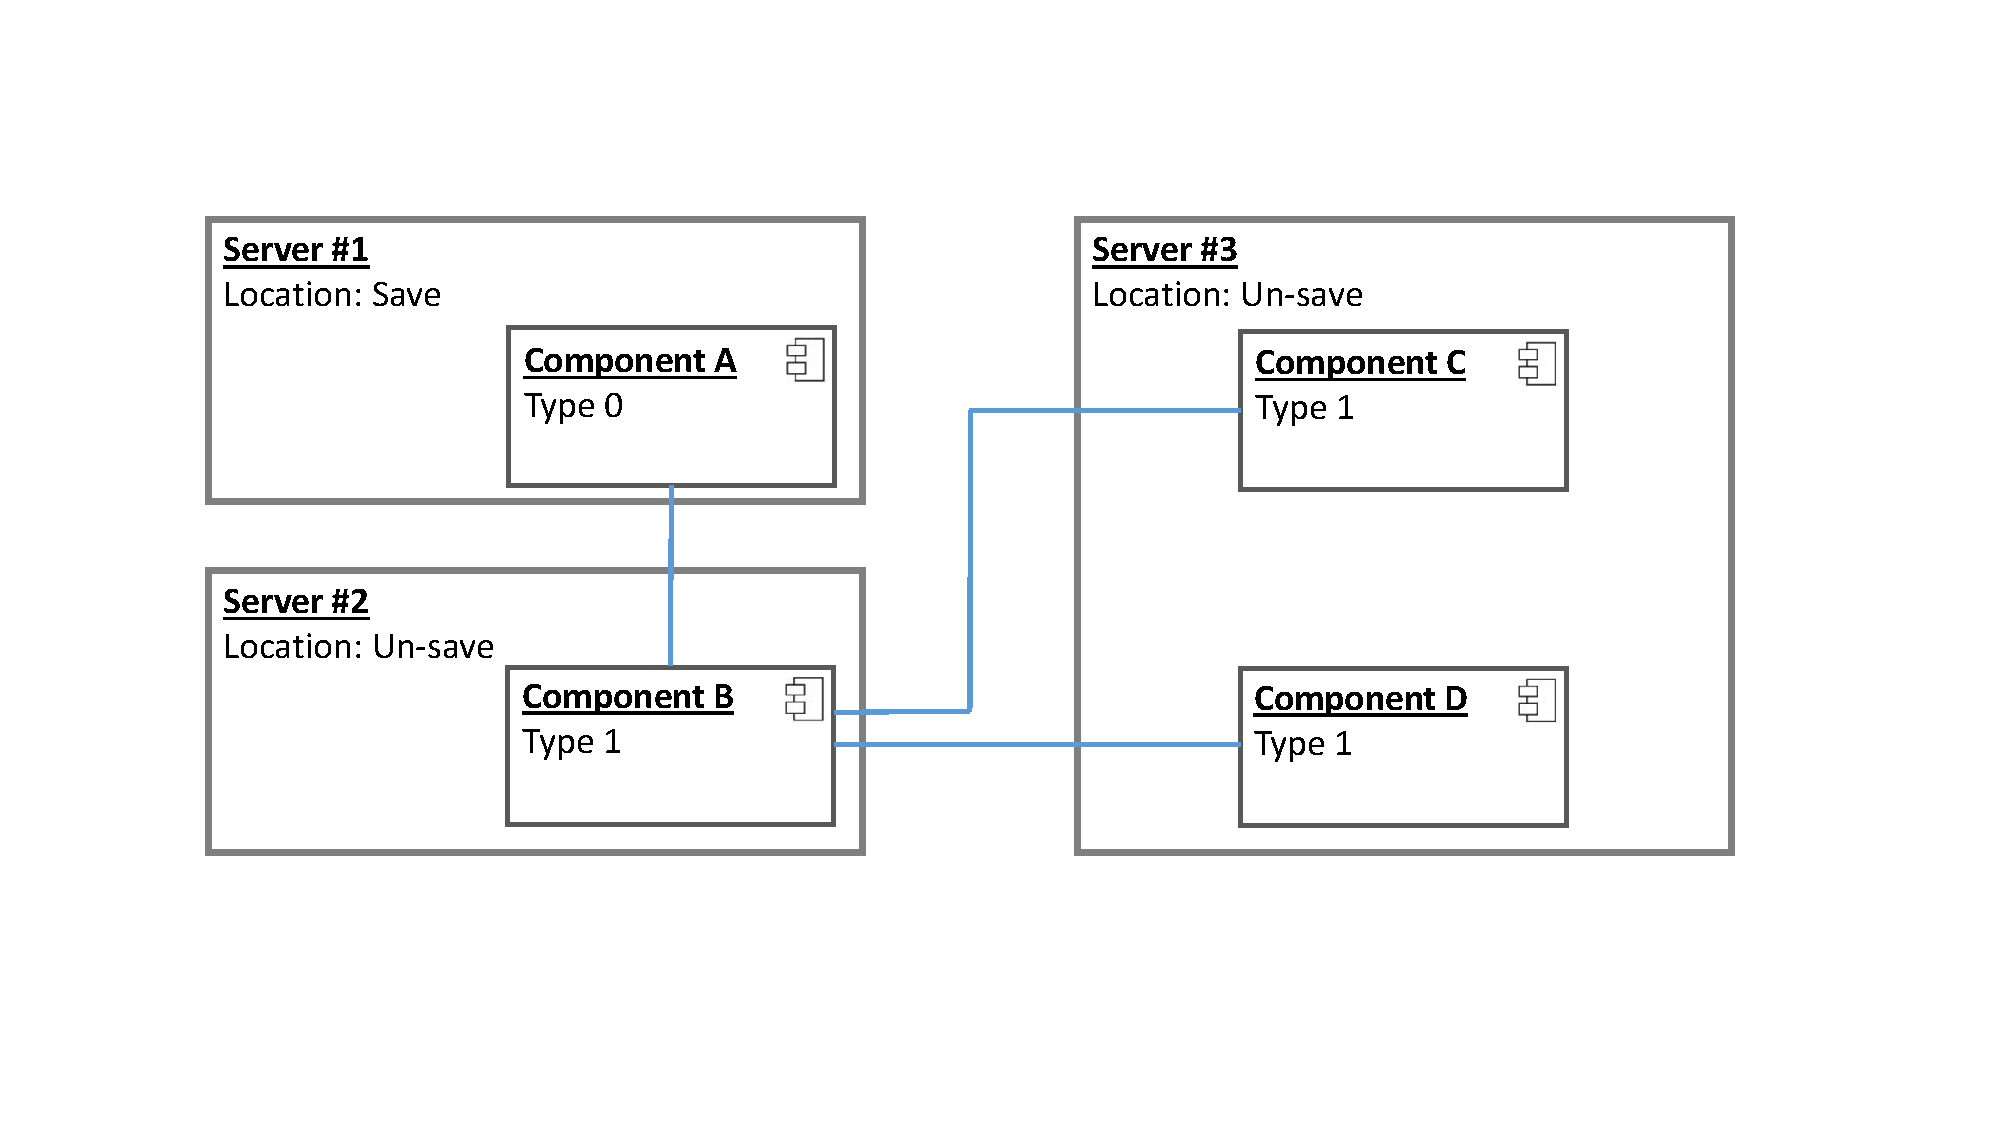
\includegraphics[trim = 35mm 45mm 40mm 35mm, clip, width=0.6\textwidth]{graphs/deployment_example_3}
	\caption{Privacy compliant deployment}
	\label{fig:example_depl:3}
\end{figure}

(\autoref{fig:example_depl:3}) shows a privacy compliant deployment. Due to, Component C and D sharing the same data source (Component B), which already only contains type 1 data. As a result, Component C and D can only contain data, already obtained by Component B. This means, even through data combination and extensive data analysis, no privacy concerning information can be extracted.


\section{Component categorization}
\label{sec:PrivacyConcept:comp_cat}

Components can be very complex due to multiple communication partners and dozens of interfaces. In such cases it can be considered impossible, to keep track of every single information flow on every component. This shows, that a component shouldn't be categorized by hand.

In contrast, a single data stream between two components is easy to understand and easy to analyse. In a component based software architecture, data exchange happens via component interfaces. During system composition the software architect must be aware of what data he passes through an interfaces.

As a result, the decision was made to categorize each interface communication during system composition. The components privacy categorization is then derived by evaluating the components communication.

We need to point out, that this categorization is only valid with the \textit{Closed World Assumption} (CWA) \cite{Sequeda.CWA}. Simplified, the CWA states, that if a system doesn't contain any information about a given statement, this statement is automatically wrong. Applied onto the privacy concept this means: The model contains all the information and information sources that exist. Naturally, this assumption is wrong, since every component may be connected to the internet and can access a nearly infinite amount of data. However, we need the CWA, in order to be able to make any statement about the systems privacy compliance. Considering the limited information we have available, the system architecture model, the statement we are providing can be considered outstanding, even while using the CWA.


\section{Information storage}
\label{sec:PrivacyConcept:pcm}

We are using the Palladio Component Model (\autoref{sec:Foundations:pcm}), which is just one of several Architecture Description Languages. Most ADLs share a comparable structure, which can differ, due to the designated purpose. We will describe the storage exemplarily on the PCM.

The runtime model is supposed to reflect every relevant information, concerning the models purpose. As a result, we need to store the components privacy level and the servers geo-location in the PCM model.

The geo-location belongs to a server, which is part of the resource environment model in PCM. The resource environment contains resource containers, which represents a server or virtual machine. So the resource container is the perfect place for storing the severs geo-location.

As mentioned in \autoref{sec:PrivacyConcept:comp_cat}, we need to categorize the communication between two connected component interfaces. The PCM system model uses the Assembly Connector to connect two component interfaces. This is the optimal model element to store the data privacy level for the inter interface communication.

%The PCM meta-model provides the repository model for component and interface specification. These are abstract and can be designed for multi-purpose usage. A database component for example can store any kind of data. This means a categorization during specification is not possible. This makes the repository model the wrong place to store the data privacy level. The system model represents the whole software system structure during runtime. This means, the purpose of a component and its neighbours are known and defined. This makes it ideal for data privacy marking.




%\todo{@Robert: Describe in view of a generic ADL or related to Palladio? CON ADL: To generic, could be anything! CON Palladio: Topic of Section PCM Extension}
%Since our base application iObserve uses the Palladio Component Model (\autoref{sec:Foundations:pcm}) we need to get the components data privacy type into the model. At first glance, this seems straight forward: Save the Data Privacy Level during design time as a components attribute. This however isn't a good solution, since the a components purpose is often not as clear as it seams. A database component for instance can contain personal, type 0 data or anonymous, type 2 data, pendent on its actual usage. As a consequence privacy levels should be applied during the system composition phase. In Palladio represented by the system model. This enables the system architect to classify two instances of the same component type differently.

%Components can be very complex, which usually results in a complicated and unintuitive data-flow. In such cases it can be considered impossible, to keep track of every data stream at once. This shows us, that a component as a whole shouldn't be categorized, but the "data-exchange points". These points are interfaces and represent the communication paths between components. While good interface designs share the same abstract multi-purpose intention as components - during design time. However, while composing the software system, it must be very clear to a software architect, what kind of data are transmitted between interfaces. In the PCM system model, provided interfaces and required interfaces are connected via an Assembly Connector. This is the optimal model element for categorizing the communicated data.
%% LaTeX2e class for student theses
%% sections/content.tex
%% 
%% Karlsruhe Institute of Technology
%% Institute for Program Structures and Data Organization
%% Chair for Software Design and Quality (SDQ)
%%
%% Dr.-Ing. Erik Burger
%% burger@kit.edu
%%
%% Version 1.3, 2016-12-29

\chapter{Overview}
\label{ch:Overview}

In this chapter we will give an overview on the system developed during this thesis and the according research. The system is massively extending iObserve, while keeping its original purpose, see \autoref{sec:Foundations:iobserve} for the fundamentals. All extensions are made for accomplishing the goals, defined in \autoref{sec:Introduction:goals}. The extended iObserve is mostly referenced as \textit{iObserve Privacy} during this thesis. iObserve Privacys architecture is a filter pipeline, where each filter represents one stage of the MAPE feedback loop (\autoref{sec:Foundations:mape}).


\begin{figure}[h]
	\centering
	\includegraphics[width=0.99\textwidth]{pictures/pipeline}
	\caption{iObserve Privacy pipeline}
	\label{fig:pipeline}
\end{figure}

The initial step, monitoring, is provided by the original iObserve. However, it doesn't support any information on the components geo-location. This extension is made directly in the original iObserve and Kieker. Upon detected geo-location or deployment changes, the runtime model gets updated and the next filter stage is invoked. We have determined the required data for a privacy analysis and provide a suited transformation of these information onto the PCM Privacy runtime model.

The compliance checker, mostly referenced as \textit{Privacy Analysis}, represents the analysis phase in the MAPE loop. It analyses the current runtime model for privacy violations. The fundamental principles were discussed in \autoref{ch:PrivacyConcept}. When a privacy violation is detected, the MAPE Planning phase gets activated.

The planning stages task is to find a privacy compliant redeployment model. For this job PerOpteryx is used. PerOpteryx (\autoref{sec:Foundations:peropteryx}) is a complex model generation and optimization framework. However, PerOpteryx doesn't support privacy or deployment constraints and therefore needs an extension. Furthermore, an output model needs to be selected as the final redeployment candidate, which gets transmitted to the final pipeline filter stage.
\todo{Add research accomplishments}

The execute phase of the MAPE loop compares the redeployment model to the runtime model. Based on this, a migration plan gets calculated and finally executed. The execution exists of several parametrized function and script calls. After the stages execution the observed software system needs to be in privacy compliant state.
\todo{Add research accomplishments}


\todo{@Robert: Add actual implemented pipeline UML with details, like SnapshotBuilder?}
%% LaTeX2e class for student theses
%% sections/content.tex
%% 
%% Karlsruhe Institute of Technology
%% Institute for Program Structures and Data Organization
%% Chair for Software Design and Quality (SDQ)
%%
%% Dr.-Ing. Erik Burger
%% burger@kit.edu
%%
%% Version 1.3, 2016-12-29

\chapter{PCM Extension}
\label{ch:pcmExtension}

As mentioned in Foundational Work the Palladio Component Model (\autoref{sec:Foundations:pcm}) was designed for early architectural performance analysis. On this basis, the PCM was modified many times to fulfil many adjacent tasks. Contrary to a modification, we decided to extend the existing PCM meta-model. This enables us to keep compatible with the existing Palladio Models and other Palladio applications.

\section{General}
\label{sec:pcmExtension:general}

The standard Palladio meta-model is insufficient for privacy compliance analysis. To save the required information, an extension is the best practice approach. The extension was designed to be as minimal invasive as possible and to keep the adaptation effort for existing Palladio models to a minimum.

Our extension is based on deriving the PCM meta-model entities. This way the new models stay compatible to other PCM applications like the Performance Simulators or PerOpteryx. Further, other extension possibilities like the \textit{steriotype} extension needs to be updated with every PCM meta-model update. This is not necessary, when the model is derived. Only changes in reference structure require the derived model to apply minor alterations. For details on referencing and modularizing in meta-models see \cite{Strittmatter.2015}.

The concept was described in \autoref{sec:PrivacyConcept:pcm}.

\begin{figure}[h]
	\centering
	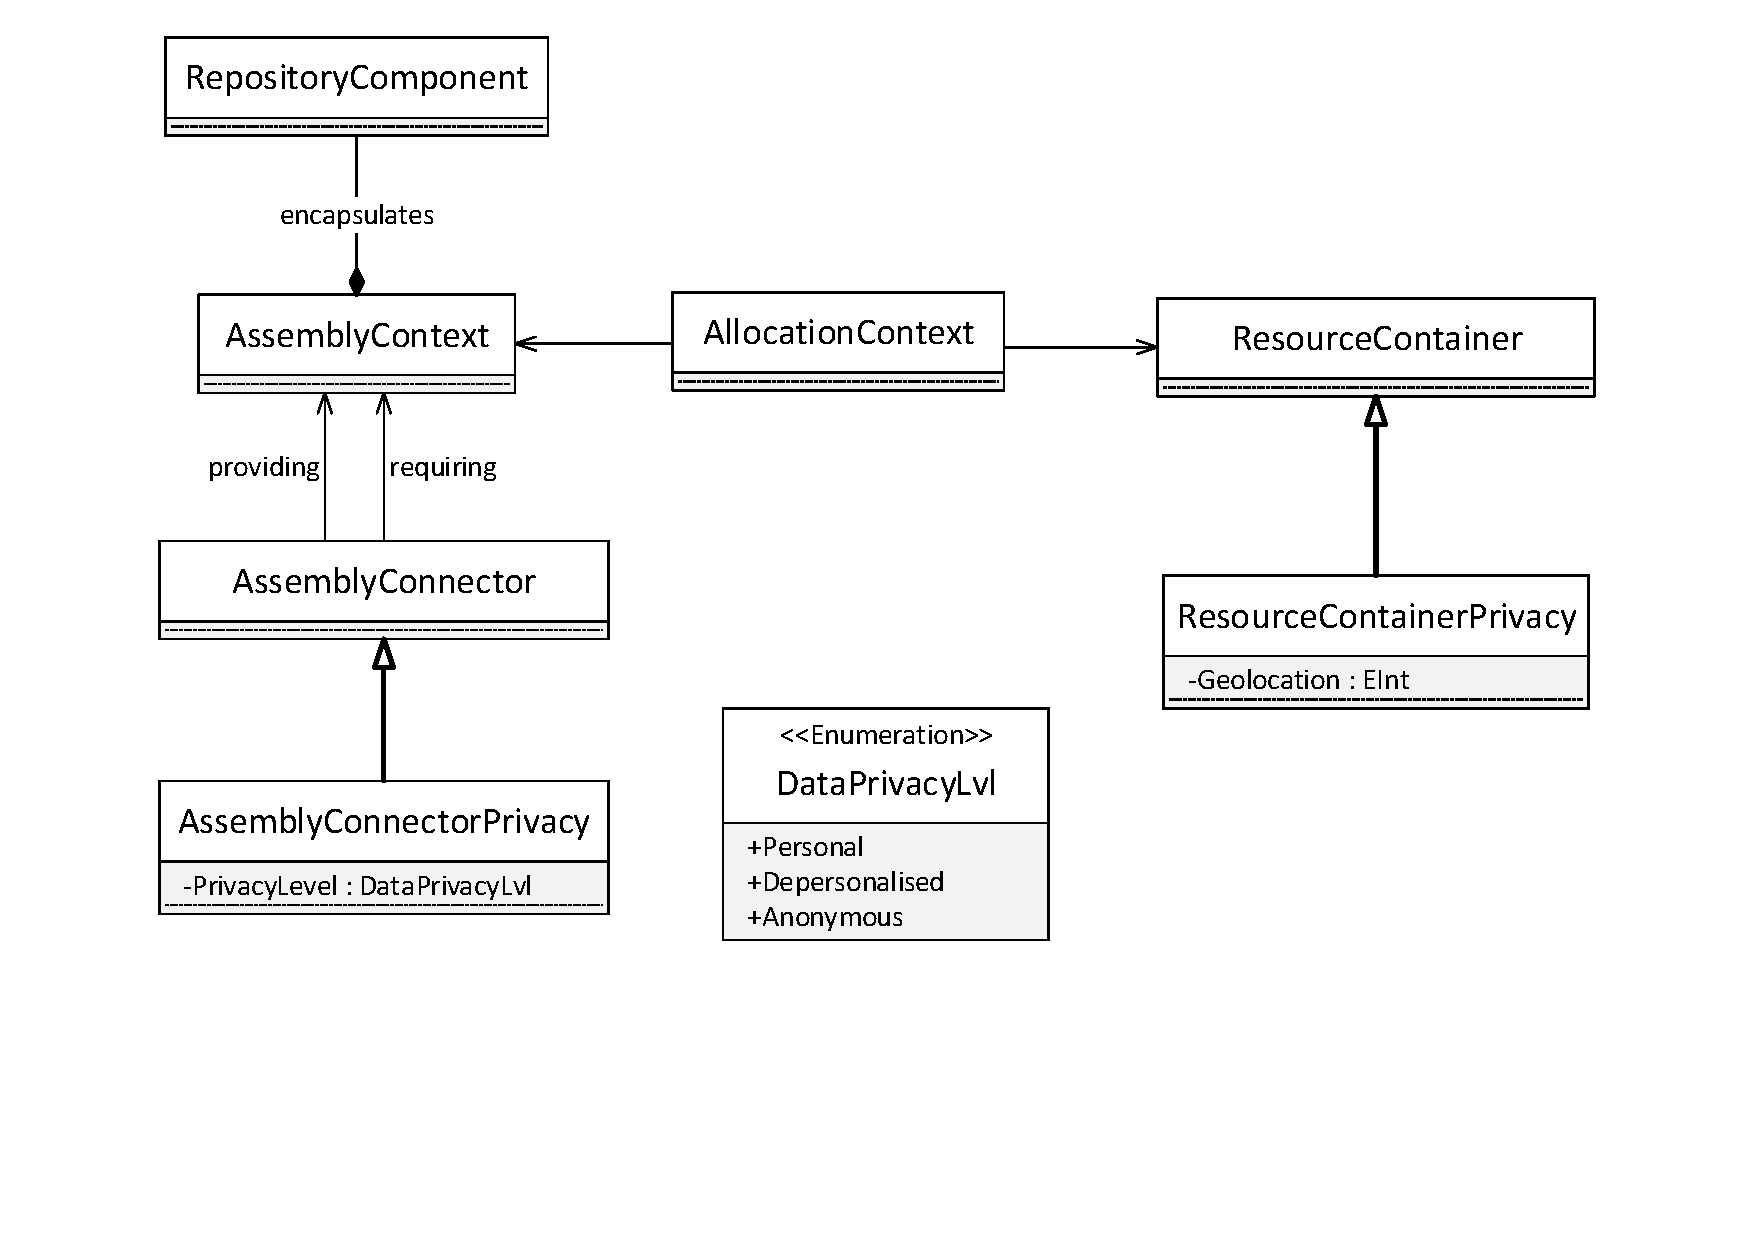
\includegraphics[trim = 20mm 50mm 20mm 05mm, clip, width=0.85\textwidth]{graphs/pcm_privacy_meta}
	\caption{PCM Privacy meta-model}
	\label{fig:pcmExtension:meta}
\end{figure}


\section{Implementation}
\label{sec:pcmExtension:impl}

The Palladio meta-model was modelled with the Eclipse Modeling Framework [EMF]. So, our extension, namely \textit{PCM Privacy}, is also modelled with EMF and references the original Palladio meta-model. The required classes were extended in corresponding sub-packages.

As described in \autoref{sec:PrivacyConcept:pcm}, we need to save a servers geo-location. The Resource Container was extended and the attribute \textit{Geolocation} added. The derived element is named \textit{Resource Container Privacy}. The geo-location itself is saved as an EInt Ecore type, a standard integer, encoded in the ISO country code (ISO 3166-1 \cite{Wikipedia.ISO_3166}). By using an integer encoded international standard we stay wildly compatible with other applications. Further, potential error sources like spelling differences, shifting borders and name changes are avoided.

The \textit{Assembly Connector Privacy} is derived from the Assembly Connector and saves the data privacy categorization. The attribute is designed as an EEnum Ecore type, with the values Personal, Depersonalized, Anonymized. This way, extending the potential categorization values requires minimal effort and is less error then a dynamic categorization via a float or an integer value. The value \textit{Personal} is set as default, to provide a over-estimation towards the legally compliant categorization, when the categorization if a connector was not performed. \autoref{fig:pcmExtension:meta} shows a simplified PCM meta-model with the three added privacy elements.


%To ensure privacy compliance, the geo-location of a component is required. In Palladio a system component is deployed onto Resource Containers. So, the Resource Container is the model equivalent of a physical/virtual server. This makes it the conceptual storage unit for the geo-location. Thus, a components geo-location can be determined via the Resource Container it is deployed on, namely the deployment model. The geo-location itself is saved as an EInt Ecore type, a standard integer, encoded in the ISO country code.

%A PCM is designed in multiple steps. Initially, interfaces for the components must be designed, followed by components and composite components. These are saved in the PCM repository model. The actual PCM system model, representing the software system, references components from the repository model. These are then connected via Assembly Connectors. While components and composed components in the repository must be deployed as a whole onto one Resource Container, components which are connected via Assembly Connectors in the system model, can be deployed on different Resource Containers. This makes the Assembly Connector the optimal model entity for categorizing the exchanged data regarding the privacy level. 


%% LaTeX2e class for student theses
%% sections/content.tex
%% 
%% Karlsruhe Institute of Technology
%% Institute for Program Structures and Data Organization
%% Chair for Software Design and Quality (SDQ)
%%
%% Dr.-Ing. Erik Burger
%% burger@kit.edu
%%
%% Version 1.3, 2016-12-29

\chapter{iObserve Extension}
\label{ch:iObserve}

iObserve was briefly introduced in \autoref{sec:Foundations:iobserve}. iObserve uses Kieker (\autoref{sec:Foundations:Kieker}) to gain real-time information about an observed (distributed) software system. iObserve transforms these information onto a Palladio Component Model. This model is referenced as \textit{runtime PCM} or \textit{runtime model}, since it reflects the actual observed software system during runtime. \cite{Heinrich.2016}


\section{Kieker}
\label{sec:Kieker:privacy}

\textit{Kieker} was also briefly introduced in foundational work (see \autoref{sec:Foundations:Kieker}). Kieker had already specified the geo-location record for transporting the geo-location information form the observed system to Kieker. However, a probe was still missing. As a result, we created a heart-beat/periodic probe (\textit{ServerGeoLocationSampler}). This probe uses a \textit{ICountryInvestigator} to determine the actual geo-location and creates creates a \textit{ServerGeoLocation} record (see \autoref{fig:geoLocationRecord}).

As an alternative, we could have created an event-based geo-location probe. A possible event could have been the component deployment or un-deployment. This however, would mean, there wouldn't be a geo-location update between these events an potential privacy violation could stay undetected indefinitely or for a long period. Even though a heart-beat probe often takes longer to send an initial record, eventual changes will definitely be detected due to the regular updates.

\begin{figure}[h]
	\centering
	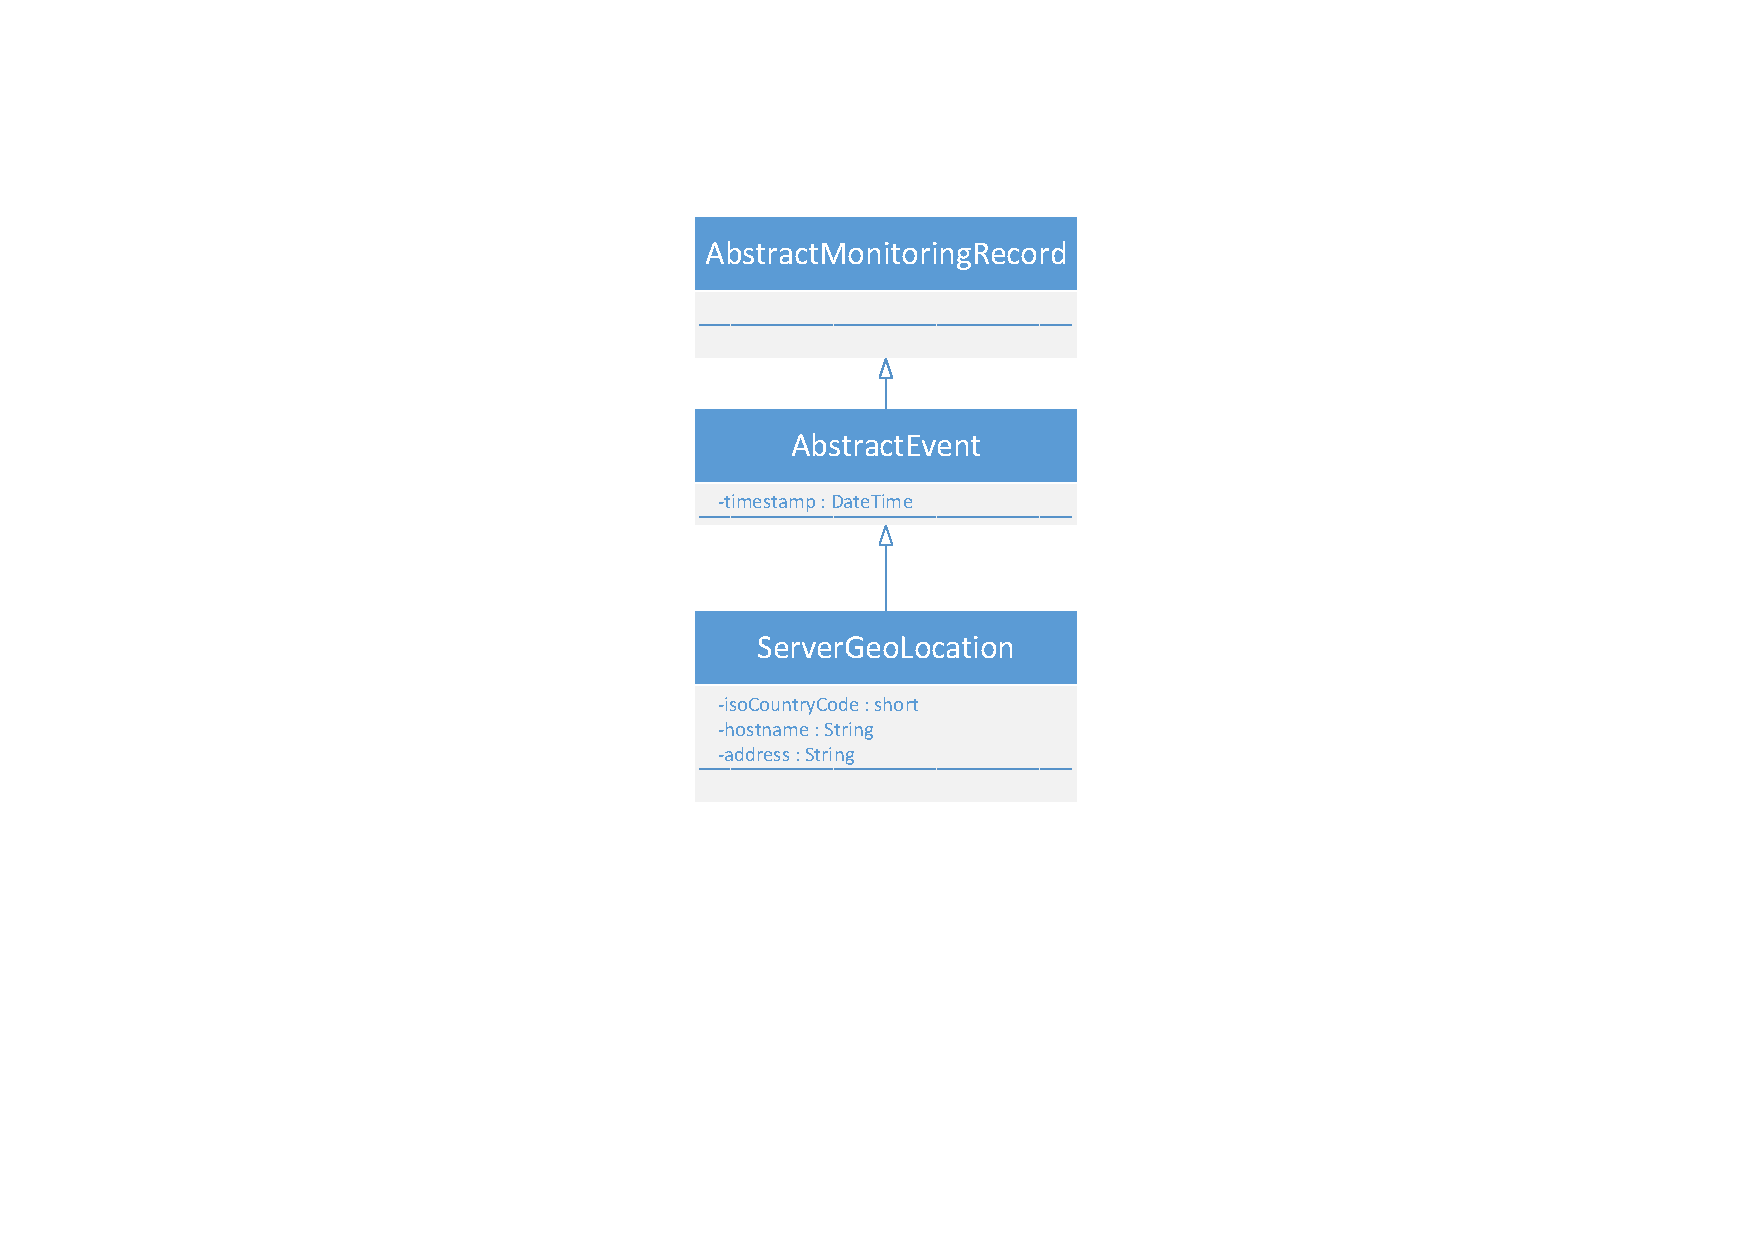
\includegraphics[trim = 20mm 70mm 20mm 20mm, clip, width=0.95\textwidth]{graphs/GeoLocationRecord}
	\caption{Server Geo-Location Record and Sampler}
	\label{fig:geoLocationRecord}
\end{figure}

Kieker gather the information from the observed system probes and redirects them to iObserve. More information on Kieker can be found at \cite{kieker.web}.

\section{iObserve Privacy}
\label{sec:iObserve:privacy}
%Kieker => Map onto PCM (Transformation)

iObserve uses the teetime framework. Its allows easy pipeline building by connecting matching input and output ports during runtime \cite{teetime.16.05.2017}. This mechanism is used by iObserve to invoke different transformations. Based on the received \textit{Monitoring Record}, the according output port gets invoked and the matching transformation will be executed.

%Geo-location transformation
For the \textit{ServerGeoLocation Record} (see \autoref{fig:geoLocationRecord}) another output port and transformation was added. The transformation uses the records host and address field to find the record sending resource container. The according geo-location attribute of the \textit{Resource Container Privacy} is compared to the incoming geo-location and updated if needed.

%Extend Framework
\begin{figure}[h]
	\centering
	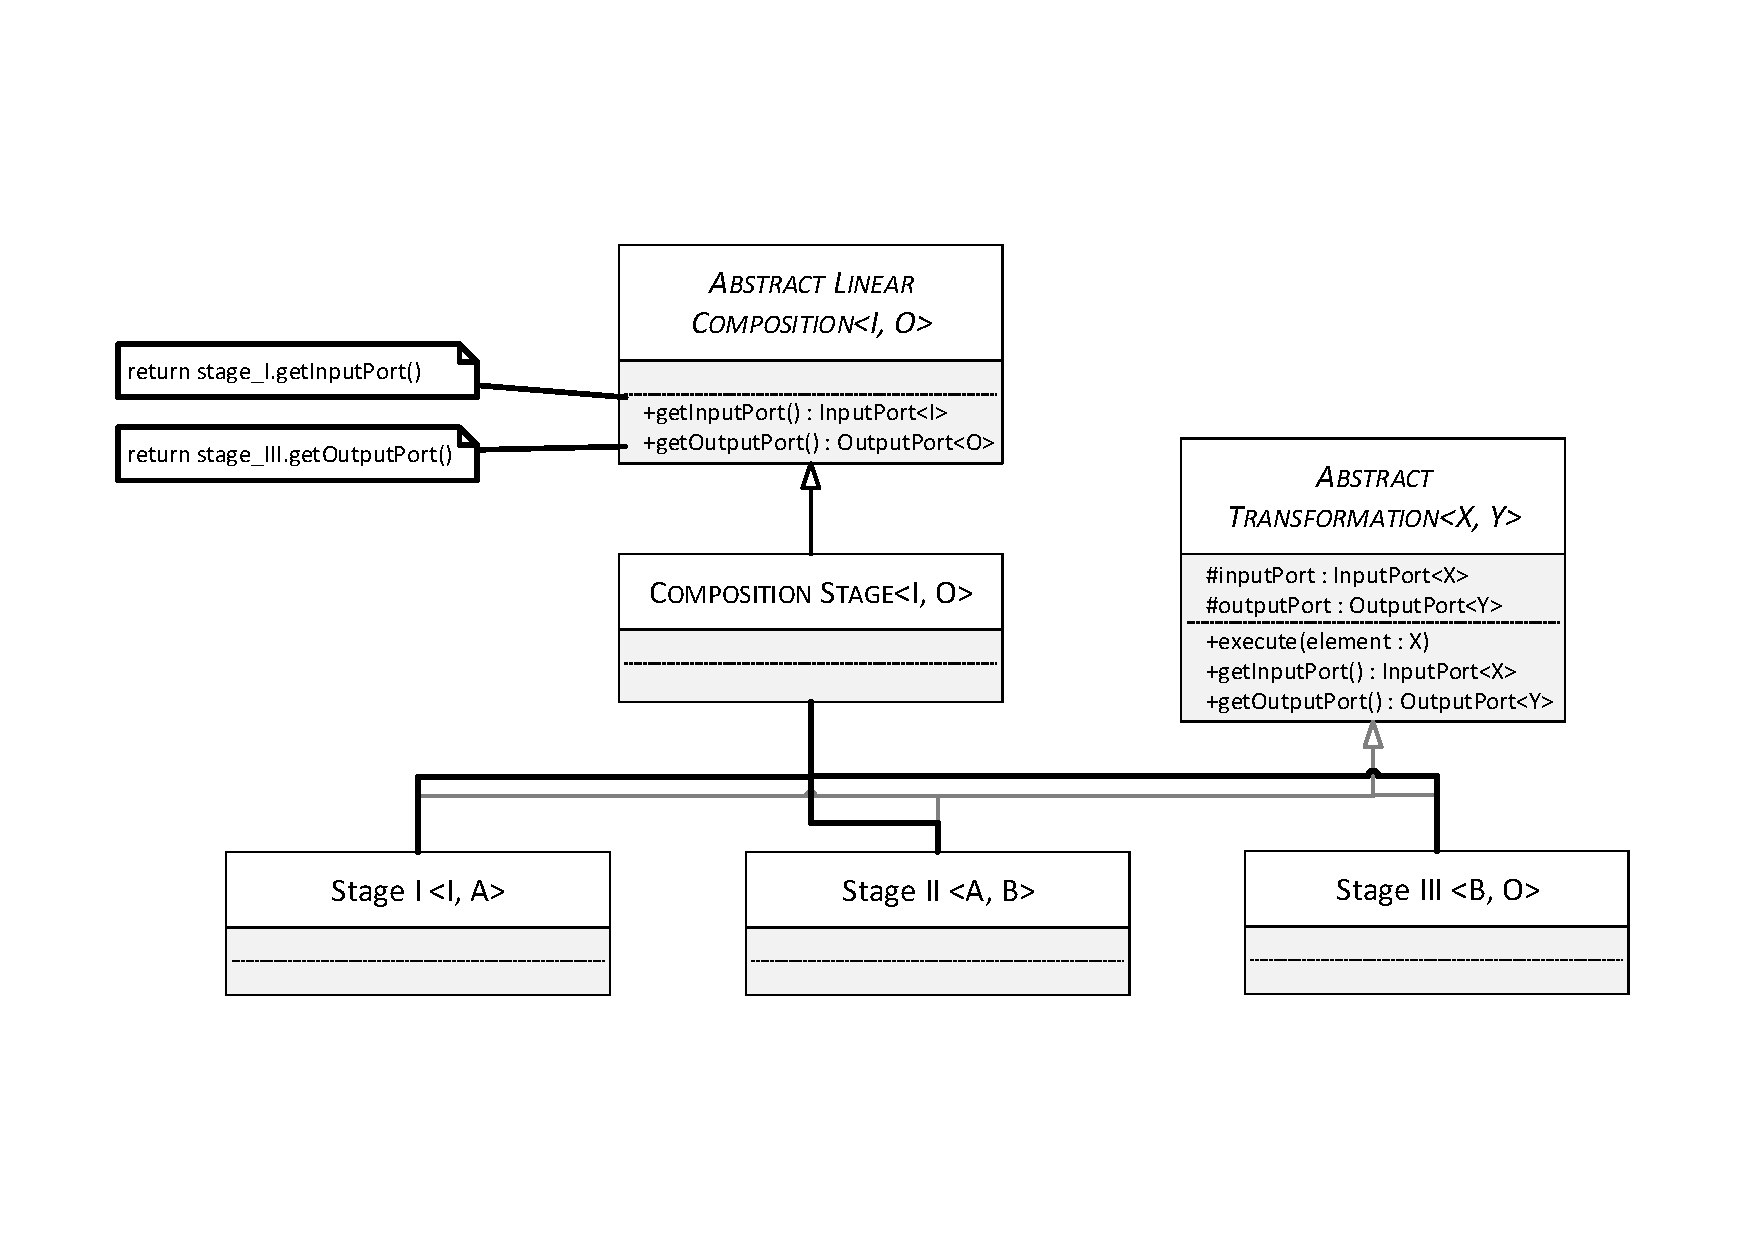
\includegraphics[trim = 20mm 40mm 20mm 35mm, clip, width=0.85\textwidth]{graphs/StageComposition}
	\caption{iObserve Privacy Filter}
	\label{fig:filterstage}
\end{figure}

iObserve has a well defined structure due to the teetime framework. We decided to keep this structure and extend it. \autoref{fig:pipeline} shows the conceptual filter pipeline structure for our planned extension. One conceptual stage usually consists if several sub tasks. To embrace re-usability and lose coupling, we decided to keep on using the teetime framework structure and compose one conceptual stage out of several sub-stages. \autoref{fig:filterstage} shows the general structure of a conceptual stage. The \textit{Composistion Stage} functions as a wrapper for the conceptual filter, while the \textit{Stages} I to III represent the sub-tasks.

This structure does not only allow easy restructuring of the conceptual pipeline and encapsulates the sub-tasks, it also allows for simple reuse and a clear separation of concerns. 
For the teetime framework, the filter stages looks like a series of linear connected stages, while the developer gets easy to handle packages. It is worth mentioning, that Stages linked to each other require matching data. The actual task executed, must be placed inside the \textit{execute} method.

The extended iObserve contains the following conceptual filter stages: \textit{Monitoring}, \textit{Snapshot} (creates a copy of the current runtime model), \textit{Privacy Analysis}, \textit{Model Generation}, \textit{System Adaptation} and \textit{Evaluation}. In the remainder of this thesis the extended iObserve is referenced as \textit{iObserve Privacy}.




\chapter{Privacy Analysis}
\label{ch:PrivacyAnalysis}

The Privacy Analysis represents the analysis stage in the MAPE-K feedback loop (\autoref{sec:Foundations:mape}). The goal is to check whether the runtime model contains any deployment related privacy violations. The privacy concept, described in \autoref{ch:PrivacyConcept}, states that privacy analysis consist of two major tasks. First, the correct privacy categorization for each software components needs to be determined. Second, the deployment evaluation, based on the deployment rules, defined in \autoref{sec:PrivacyConcept:deploymentrules}, needs to be performed.

The remaining chapter is divided into a theoretical part (\autoref{sec:PrivacyAnalysis:theory}), a component categorization part (\autoref{sec:PrivacyAnalysis:categorization}), a deployment evaluation part (\autoref{sec:PrivacyAnalysis:deployment}) and the implementation part (\autoref{sec:PrivacyAnalysis:implementation}).


\section{Analysis Theory}
\label{sec:PrivacyAnalysis:theory}

The exclusive source of information for the privacy analysis is the systems PCM Privacy runtime model. For an efficient analysis one first need to identify the minimal required information and substitute them, depending on the available sources.


\subsection{Required information}
In the context of Privacy Analysis there is a minimum of two pieces of information which are required for privacy analysis:

\begin{table}[h]
	\centering
	\begin{tabular}{r | l}
		\hline
		\textbf{\#} & \textbf{Required information for privacy analysis}\\
		\hline
		M1 & Information on components privacy level \\
		M2 & Information on components geo-location \\
		\hline
	\end{tabular}
	\caption{Minimal information for privacy analysis}
	\label{tab:pa_minimal_info}
\end{table}

Usually \textit{M1} and \textit{M2} is not directly available. As a consequence other ones must substitute these, while containing the same information. A suitable substitution, differs based on the sources and their contained information.

The used PCM Privacy meta-model provides a data privacy categorization of the communicated information between component interfaces. This enables a component classification, based on the most critical communication with another component. As a result, a components privacy level can be determined without knowing its exact purpose, analysing any inner processes or knowing the exact data-flow. So, $M1$ gets substituted by information about inter interface communication and its privacy categorization.

In order to get an information equivalent of $M2$, a components host must be determined, as well as that hosts geo-location. The PCM Privacy model provides these information. However, it is spread over multiple models. As a result we require only four pieces of information (\autoref{tab:iobserve_information}), compared to R-PRISs six pieces of information (\autoref{tab:rpris_information}).

\begin{table}[h]
	\centering
	\begin{tabular}{r | l}
		\hline
		\textbf{\#} & \textbf{Required information to carry out runtime check}\\
		\hline
		I1 & Interactions of two components per interface \\
		I2 & Information on component deployments on physical resources \\
		I3 & Geo-location information of physical resources \\
		I4 & Data Privacy categorization per interface communication \\
		\hline
	\end{tabular}
	\caption{iObserves information for runtime privacy checks}
	\label{tab:iobserve_information}
\end{table}

\subsection{Data-flow direction}
\label{sec:PrivacyAnalysis:theory:dataflow}
Usually component interfaces are categorized into providing and requiring interfaces. Interface connections are made between a pair of required and provided interfaces of the same type. This suggests a certain data- and control-flow direction. This is a wrong assumption. While there are cases, when the control-flow can be derived from this structure, the data-flow is completely independent from this categorization.

For example, a database component (usually) only has provided interfaces. These interfaces allows the user to store and retrieve data from the database and therefore contains getter and setter methods. This means, there is no data-flow direction for the whole interfaces, since the data needs to "flow" into both directions. Note, that we are explicitly speaking of an interface as a whole, since individual methods can have a data-flow direction.

Information passed through an interface are available on the providing and requiring component. In other terms, if an component connector got categorized as \textit{Personal}, information of this type are available in both components. These components need to get categorized accordingly.

\subsection{Joining data streams}
\label{sec:PrivacyAnalysis:theory:jds}
In \autoref{sec:PrivacyConcept:deploymentrules} we elaborated on the danger of two \textit{Personally Identifiable Information} (Type 1) data streams, from two sources, joining on a single server. In such a case, the combination of these data streams could lead to personal, privacy relevant data. (Compare \autoref{enum:deployment_rules}, Rule 4). This concept applies on the described deployment level and also on the component categorization process.

While on deployment level, the information streams are not actively merged, this is a realistic possibility on the component categorization level. So the argument of applying an overestimation is not valid and this scenario must be taken seriously. In the following this special case will be refereed to as \textit{joining data streams} (short: JDS). In the following section, a couple of categorization and deployment examples will help clarifying this scenario.


\section{Component categorization}
\label{sec:PrivacyAnalysis:categorization}

The component categorization requires two tasks. The initial categorizing of every component and the analysis for with \textit{join data streams}.

The initial data privacy level of a component is equal the components most critical communication level (see \autoref{sec:PrivacyAnalysis:theory:dataflow}). This task is performed during the model graph construction. The search for joining data streams is more complex and requires a formalization, as well as an extended explanation. We will continue with the formal description, followed by an textual explanation and close with some examples.

\begin{description}
	\item{\textbf{Definitions}}
	\begin{itemize}
		\item The Graph $G := (N, E)$
		\item The Nodes $N$ consist of personal Nodes $p \in N_p$, depersonalised Nodes $d \in N_d$ and anonymized Nodes $a \in N_a$ $\wedge$ $N_p \cup N_d \cup N_a = N$ $\wedge$ $N_p \cap N_d \cap N_a = \{ \emptyset \} $
		\item The edges $E$ consist of personal Edges $e_p \in E_p$, depersonalised Edges $e_d \in E_d$ and anonymized Edges $e_a \in E_a$ $\wedge$ $E_p \cup E_d \cup E_a = E$ $\wedge$ $E_p \cap E_d \cap E_a = \{ \emptyset \} $ 
		\item Path $P = \langle(p_1, p_2, \dots, p_n), (e_1, e_2, \dots, e_{n-1})\rangle$ with $p \in N$ and $e \in E$
	\end{itemize}

	\item{\textbf{Formalization}}
\end{description}
\begin{gather*}
	\textrm{Every component is correctly categorized}\\
	\Leftrightarrow\\
	\nexists \textrm{ Path P } \textrm{ with let } {i, j} \in [0, n-1] \wedge i \neq j: e_i \neq e_j \wedge e_i \in E_d \\
	\wedge (p_2, p_3, \dots, p_{n-1}) \in N_d \wedge \{ p_1, p_n \} \in N_p \wedge n \geq 3
\end{gather*}

The formalization states, that every component in the graph $G$ is correctly categorized if no path from one personal component to a personal component exist. However, the path must traverse at least three components, while every edge is only used once and only depersonalised edges are used. Further, all internal nodes must have a depersonalised categorization.

When such a case is found, the depersonalised components of the path must be categorized as \textit{Personal}. As a result, the case is eliminated and categorization is corrected according to the \textit{joining data stream}. The following examples will illustrate the categorization and point out certain special cases.

\begin{figure}[h]
	\centering
	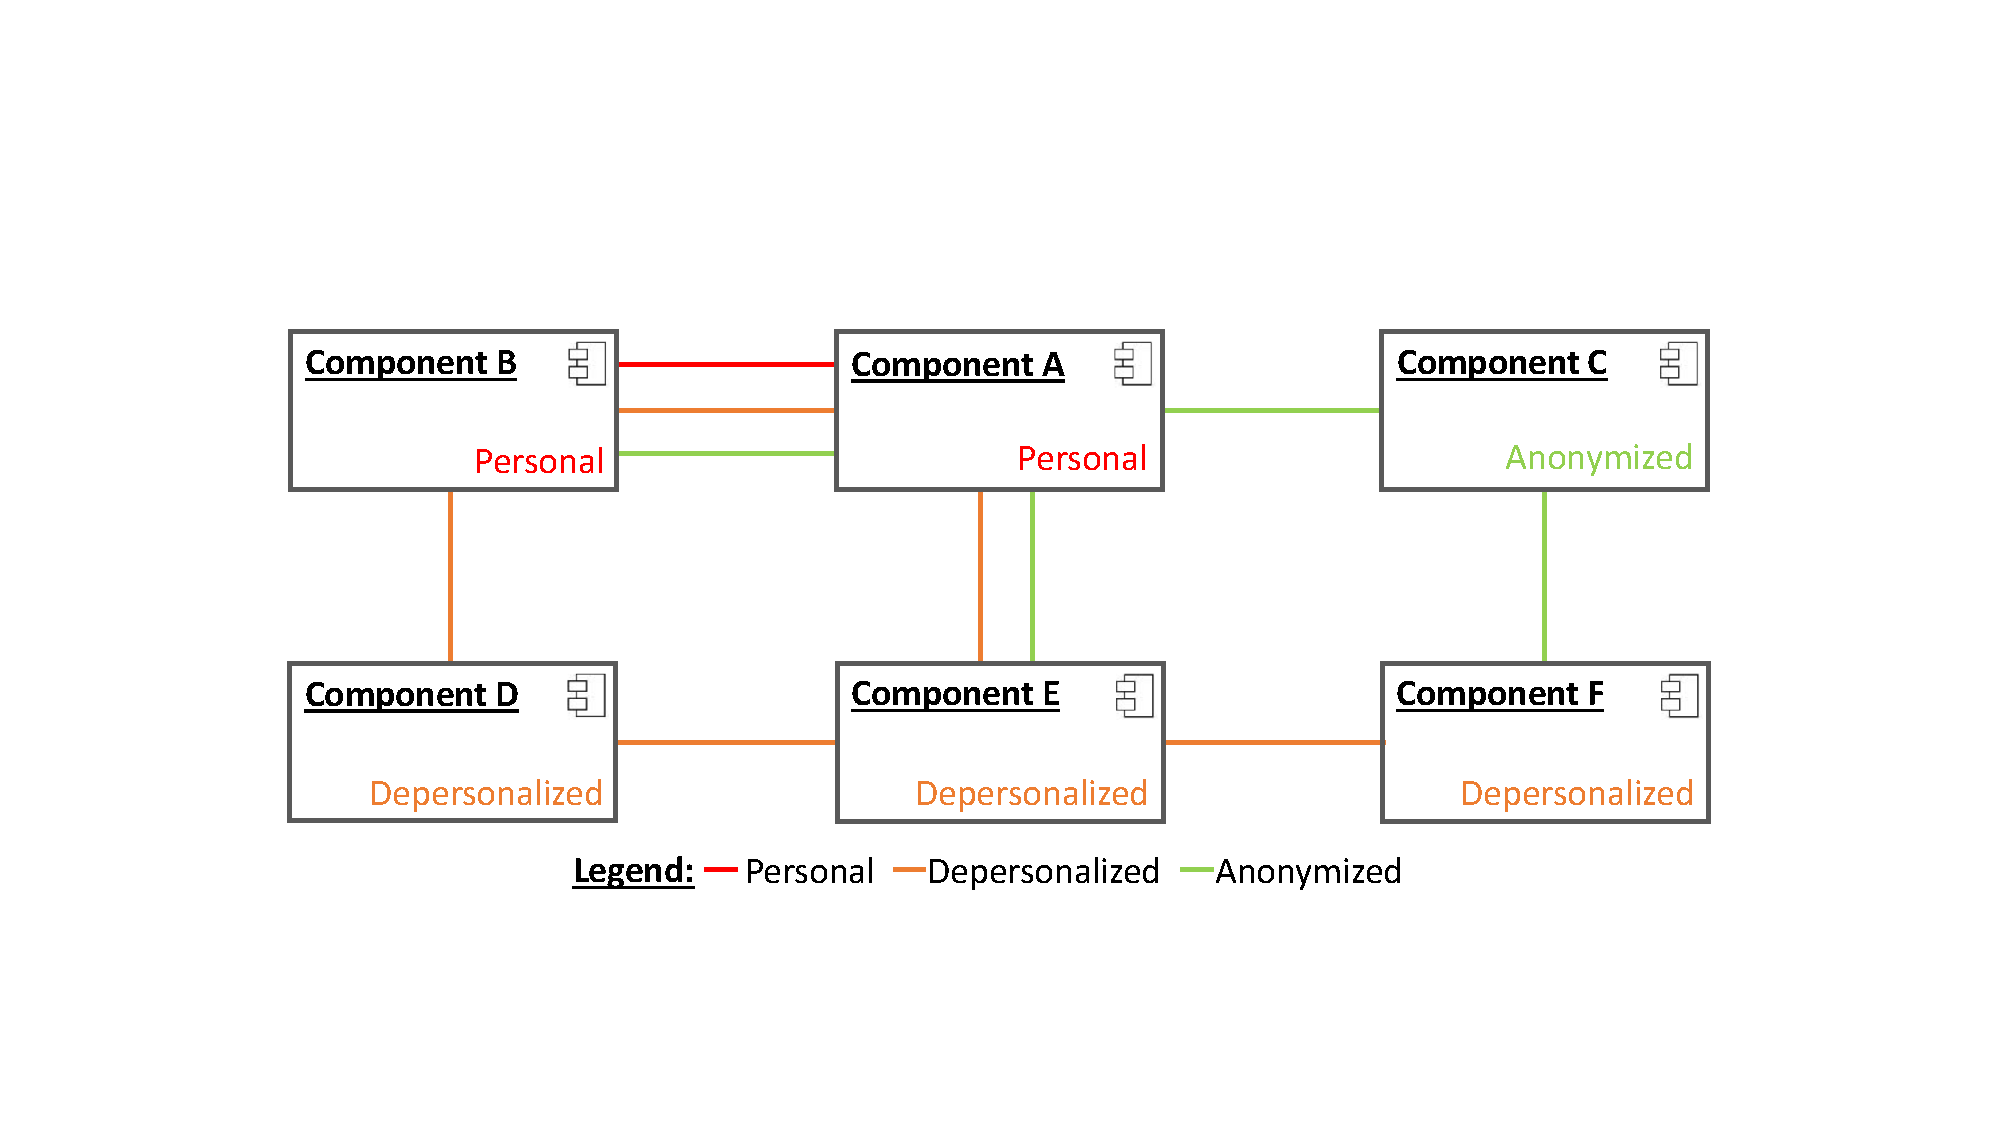
\includegraphics[trim = 35mm 40mm 40mm 45mm, clip, width=0.75\textwidth]{graphs/component_categorization_examples_initial}
	\caption{Initial component categorization}
	\label{fig:example_categorization:init}
\end{figure}

\autoref{fig:example_categorization:init} shows the components data privacy level after the initial categorization phase. \autoref{fig:example_categorization:base} shows the result of categorization analysis. The comparison of these two states show, that component D and E get "upcasted" and gain a \textit{Personal} - more critical - data privacy categorization. This is due to the fact, that component D and E have a connection onto two personal data sources (Component A and B). Applying the formalization, a path from component A to B via component E and D, using only depersonalised edges, can be found. This means, as mentioned above, a joining data stream exists and component D and E needs to be categorized as \textit{Personal}.

\begin{figure}[h]
	\centering
	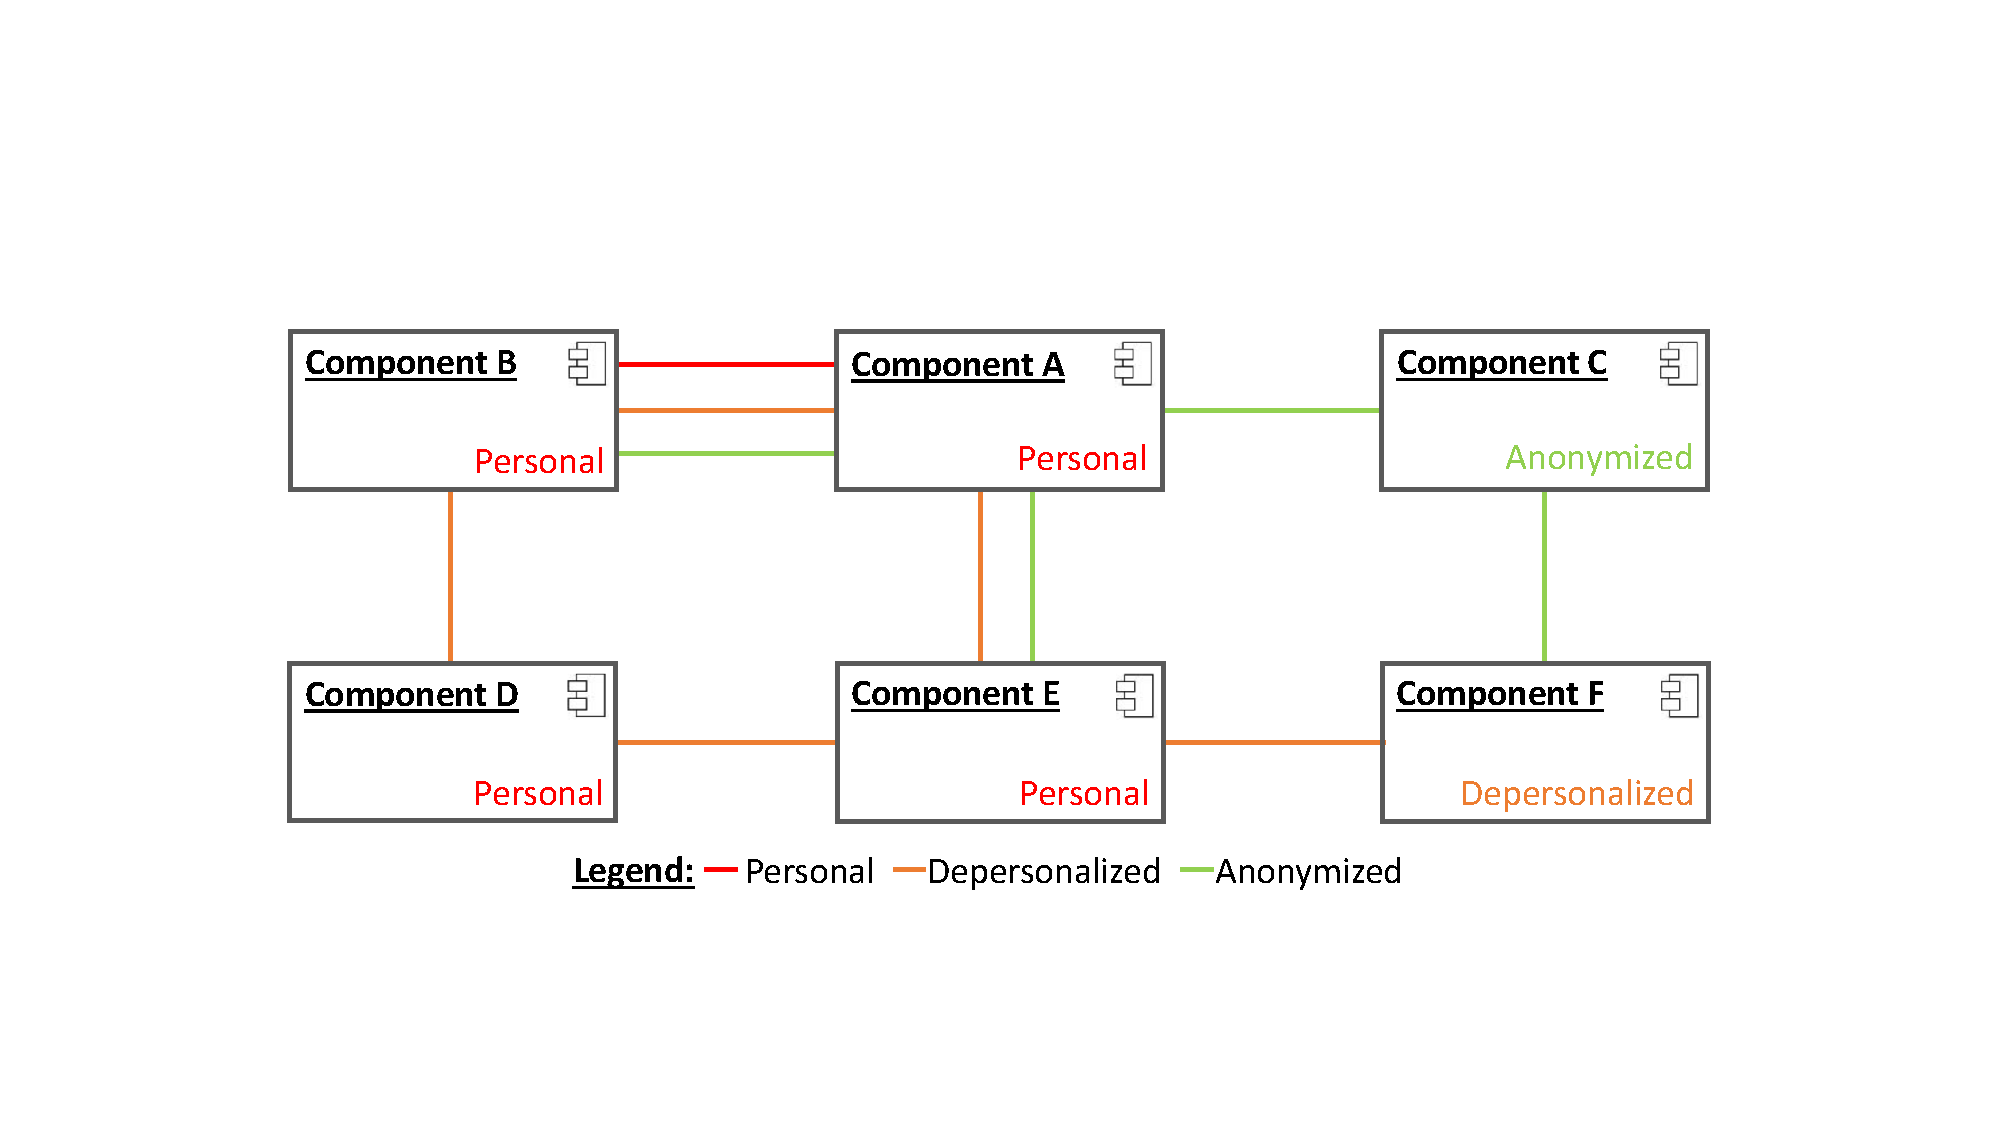
\includegraphics[trim = 35mm 40mm 40mm 45mm, clip, width=0.75\textwidth]{graphs/component_categorization_examples_upcast_base}
	\caption{Post categorization analysis - basic example}
	\label{fig:example_categorization:base}
\end{figure}

Two special cases are shown in \autoref{fig:example_categorization:advanced}. So is component D categorized as \textit{Personal} even though it has only one other component as data source. However, it has two individual connections to component B, which could contain a joining data stream, since B has a personal categorization. The formalization states, that a personal component needs to be reached, while using every edge only once. This conditions are fulfilled.

\begin{figure}[H]
	\centering
	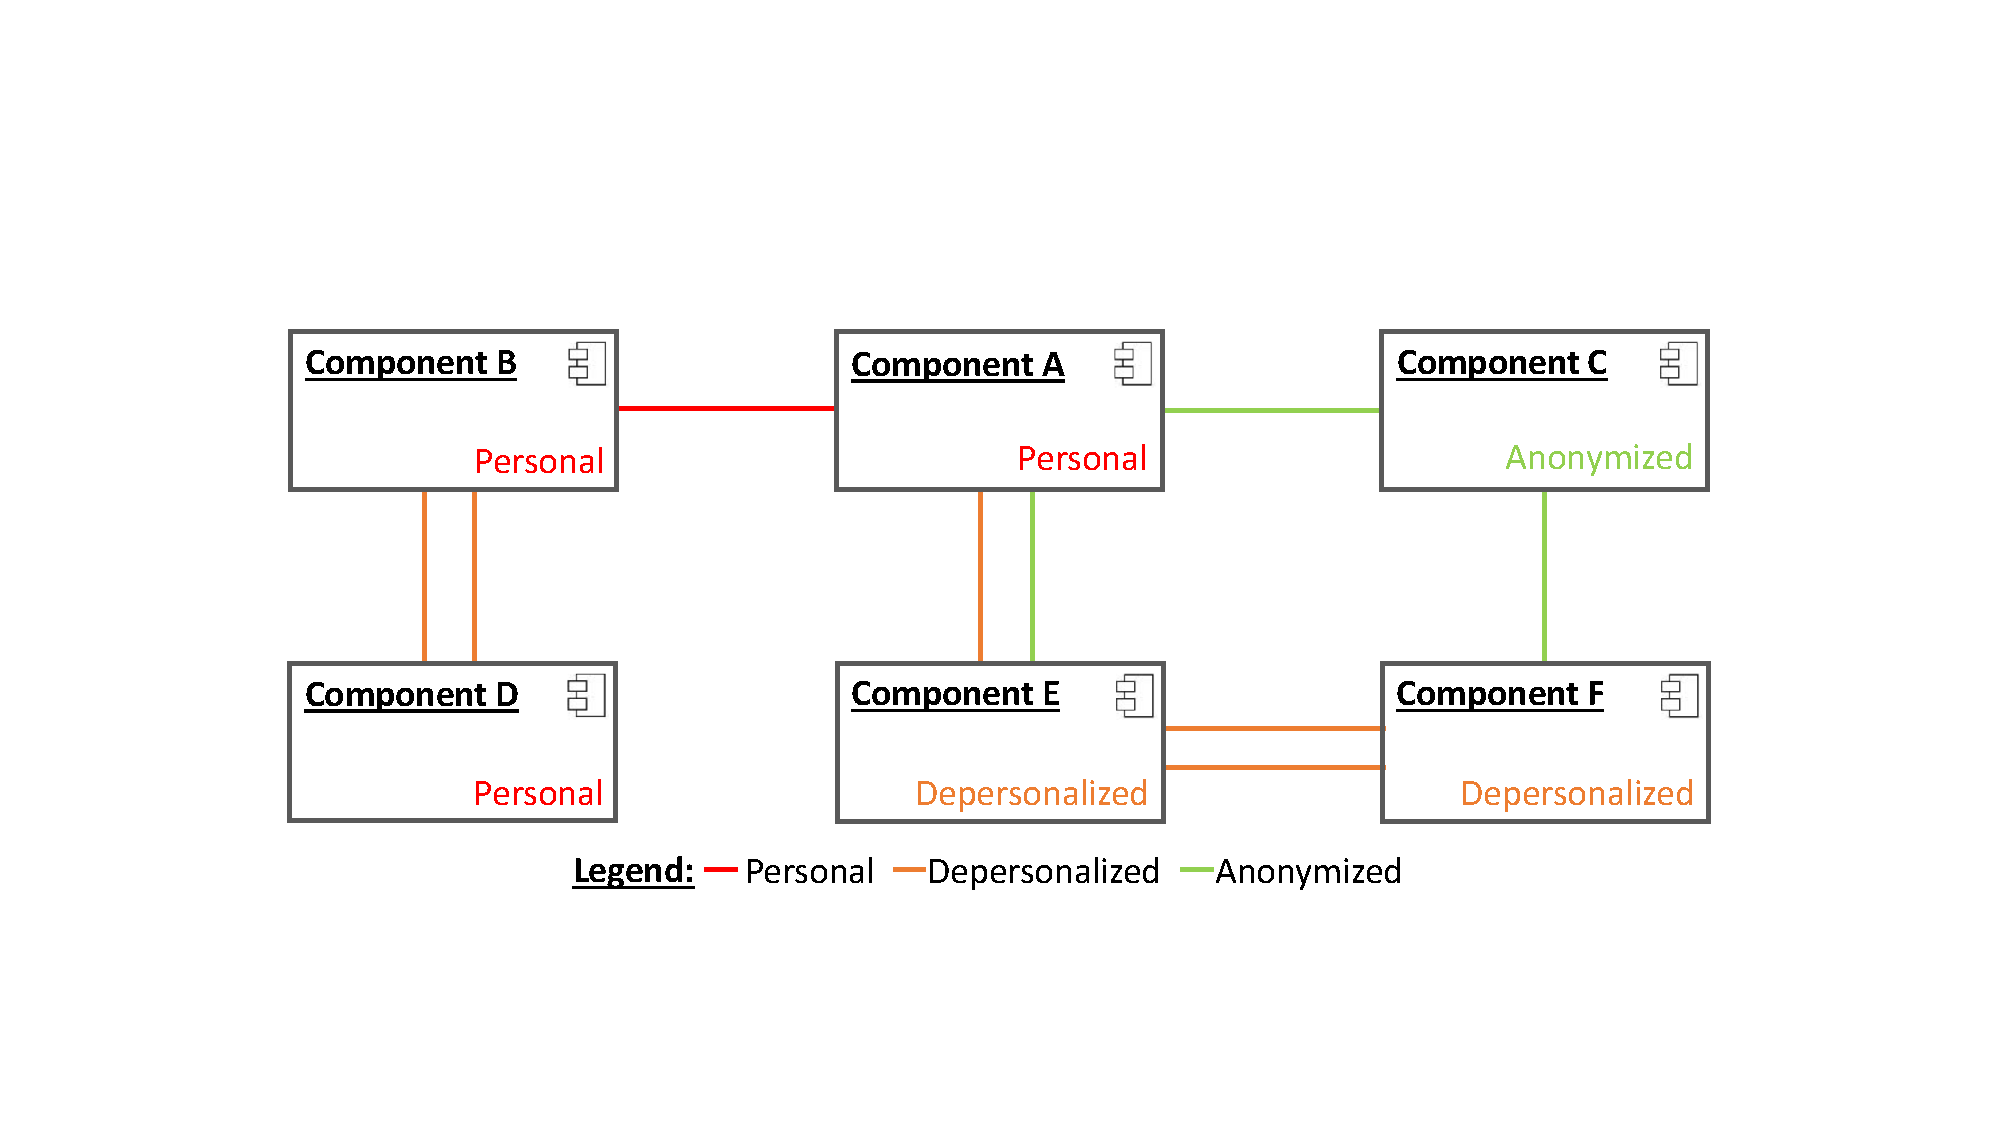
\includegraphics[trim = 35mm 40mm 40mm 45mm, clip, width=0.75\textwidth]{graphs/component_categorization_examples_upcast_advanced}
	\caption{Post categorization analysis - advanced example}
	\label{fig:example_categorization:advanced}
\end{figure}

Component F doesn't get an \textit{Personal} categorization since it can only contain privacy relevant data that are already present on component E. And component E has a depersonalized categorization. All anonymized categorized connections and components are ignored, since they don't contain any privacy related information. Applying the formalization, no path from A to a personal component can be found, using only depersonalised edges and each edge only once. So, the categorization is correct.


\section{Deployment analysis}
\label{sec:PrivacyAnalysis:deployment}

The deployment analysis' goal is to find out whether the current deployment is privacy compliant. A deployment is considered privacy compliant if no deployment violation is found. The rules for a privacy compliant deployment were described in \autoref{sec:PrivacyConcept:deploymentrules}. In the following we will formalize the deployment analysis, describe the formalization textually and finally give an example.

\begin{description}
	\item{\textbf{Definitions}}
	\begin{itemize}
		\item The Graph $G := (N, E, S)$ 
		\item The Nodes $N$ consist of personal Nodes $p \in N_p$, depersonalised Nodes $d \in N_d$ and anonymized Nodes $a \in N_a$ $\wedge$ $N_p \cup N_d \cup N_a = N$ $\wedge$ $N_p \cap N_d \cap N_a = \{ \emptyset \} $
		\item The edges $E$ consist of personal Edges $e_p \in E_p$, depersonalised Edges $e_d \in E_d$ and anonymized Edges $e_a \in E_a$ $\wedge$ $E_p \cup E_d \cup E_a = E$ $\wedge$ $E_p \cap E_d \cap E_a = \{ \emptyset \} $  
		\item The servers $S$ consist of save Servers $s_s \in S_s$ and un-save Servers $s_u \in S_u$ $\wedge$ $S_s \cup S_u = S$ $\wedge$ $S_u \cap S_s \cap N_a = \{ \emptyset \} $
		\item Let $N_{si}$ are the nodes deployed on server $s_i$
		\item Path $P = \langle(p_1, p_2, \dots, p_n), (e_1, e_2, \dots, e_{n-1})\rangle$ with $p \in N$ and $e \in E$
	\end{itemize}
	
	\item{\textbf{Formalization}}
\end{description}
\begin{gather*}
	\textrm{The deployment is illegal}\\
	\Leftrightarrow\\
	\exists n \in N_{si}: n \in N_p \wedge n \textrm{ deployed on } s_i \wedge s_i \in S_u \\
	\vee\\
	\exists s_x \in S_u \nexists \textrm{ Path  with } N_{sx} \subset P \wedge p_i \in N_d \wedge e_j \in E_d \\
	\vee \\
	\exists \textrm{ Paths } \{P_1, P_2, \dots, P_n\} \textrm{ from } N_p \textrm{ to } N_{si} \textrm{ with } i \in [0, n], j, k \in [0,|P_i|]: \\
	e_j \in E_d \wedge e_{pj} \cap e_{pk} = \{ \emptyset \} \wedge n \geq 2 
\end{gather*}

The formalization states three independent conditions for an illegal deployment. First, the deployment of an as personal categorized component on a server located in an un-save geo-location. Second, the depersonalised components on a un-save server are not connected. The potential connection must consist of depersonalised edges but can be transitive via depersonalised components and edges. The third condition states, that if there is more then one path, from the set of personal components to the depersonalised components hosted by an un-save server, then the deployment is illegal. However, must consist of individual, non overlapping and depersonalised edges.

\begin{figure}[h]
	\centering
	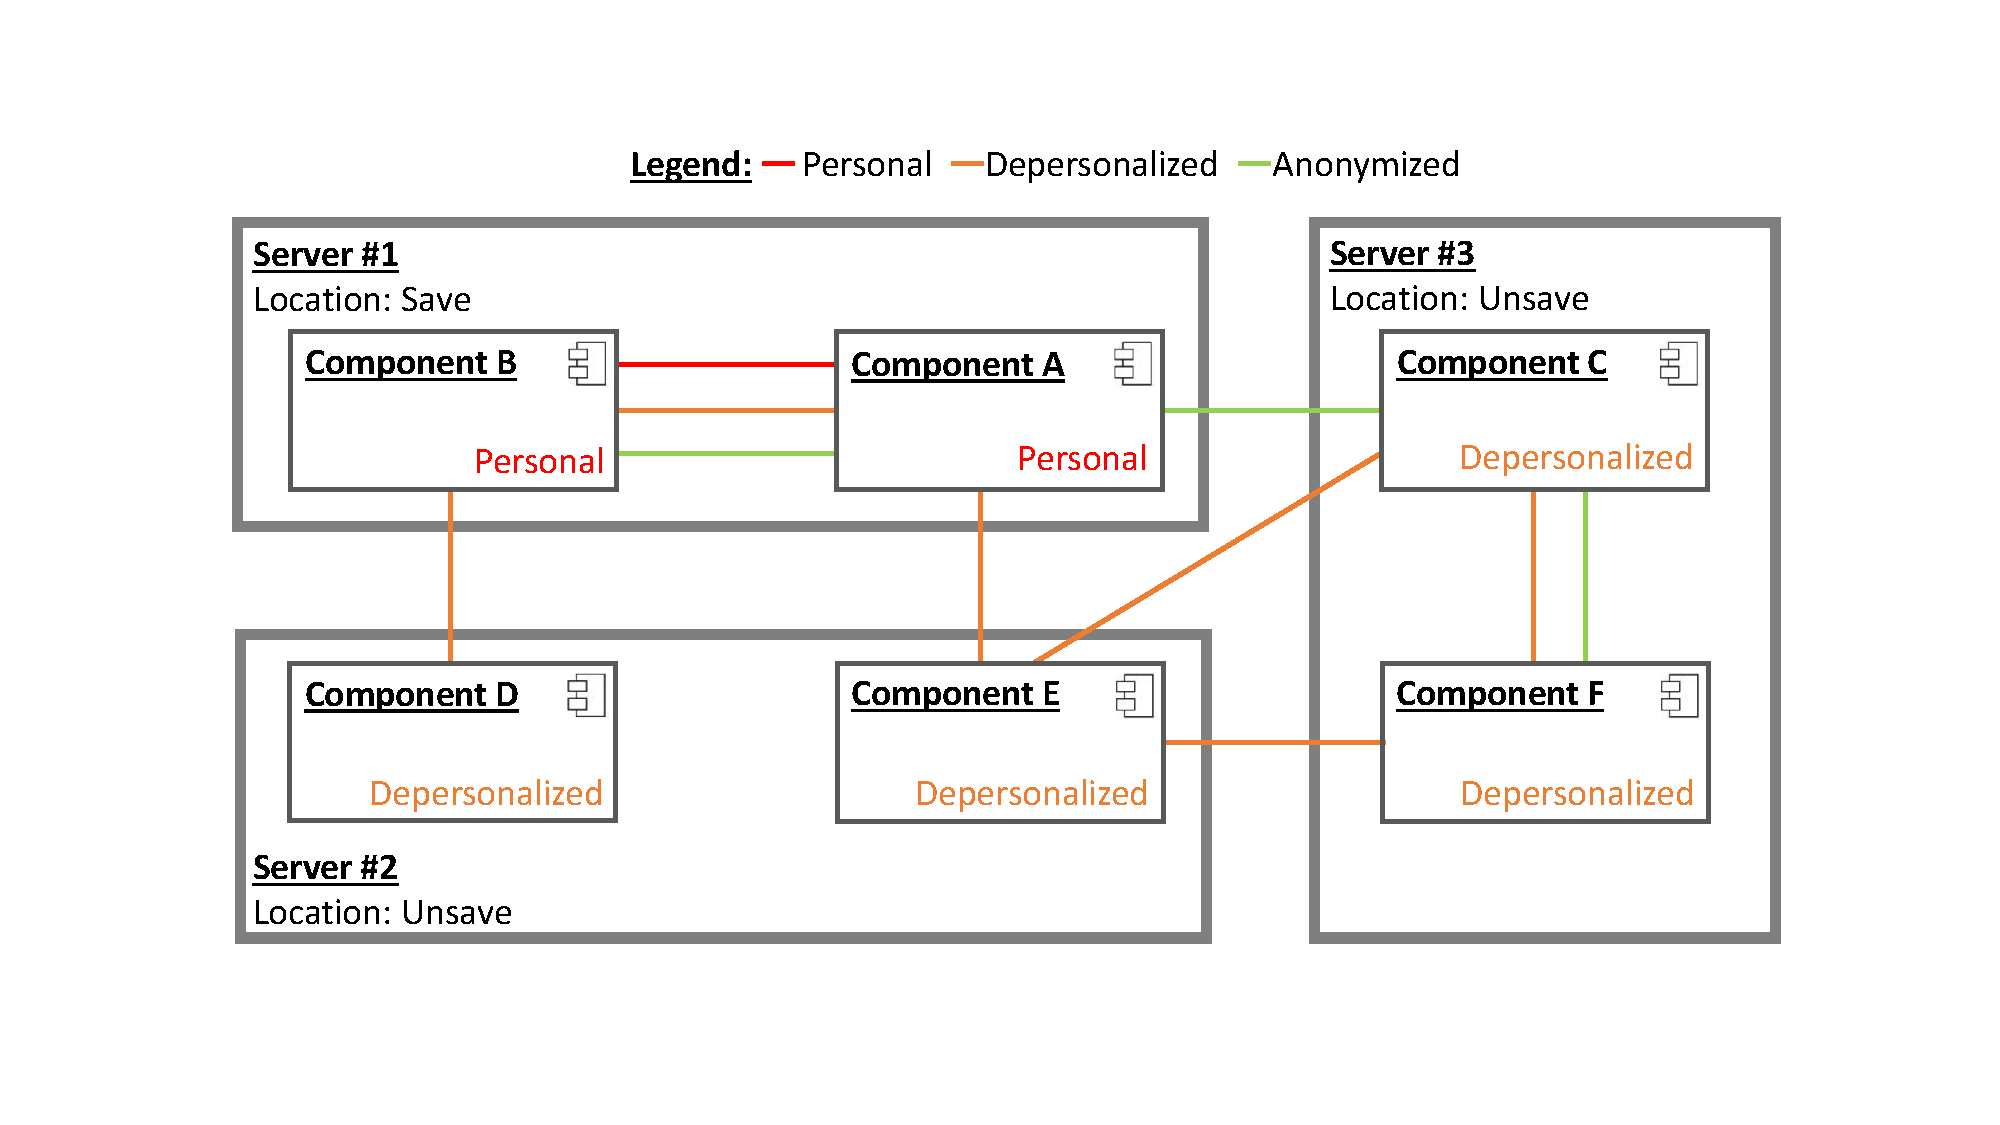
\includegraphics[trim = 35mm 30mm 30mm 25mm, clip, width=0.85\textwidth]{graphs/deployment_example_implementation_eval}
	\caption{Deployment analysis example}
	\label{fig:example_deplyoment_eval}
\end{figure}

\autoref{fig:example_deplyoment_eval} shows an illegal deployment. The deployment of Component A and B is obviously valid, due to its deployment on a "save" geo-location. Component C and F are also legally deployed, since both components share a single communication edge onto privacy relevant information and the "joining data streams" situation does not apply. Applying the formalization, the first condition is broken, since server \#3 does not host a personal component, the second condition is also false, since the components C and D are transitive and direct connected via depersonalised edges. The third condition does also not apply, since only one individual path via depersonalised edges from the personal components exists.

Server\#2, however, hosts an illegal deployment. Component D and E have different single data sources edges and can therefore save, process or transmit data, which can combine to privacy relevant data. The second and the third condition of the formal specification are true. So, are component E and D not transitively connected via depersonalised nodes. Further, two individual paths from the set of personal components to the components hosted by server \#2 exist.


\section{Privacy Analysis implementation}
\label{sec:PrivacyAnalysis:implementation}

The PCM meta-model defines multiple models, each providing knowledge about a certain aspect of the target system (see \autoref{fig:pcm_info_spread}). This is not suited for an efficient privacy analysis and therefore requires an information preprocessing. So the implementation is spread over three steps:

\begin{enumerate}
	\label{enum:algorithm_steps}
	\setlength\itemsep{0em}
	\item build efficient data structure
	\item categorize components
	\item analyse deployment
\end{enumerate}


\subsection{Information preprocessing}
\label{sec:PrivacyAnalysis:implementation:prepro}

In the first algorithm phase, all informations $I1$ to $I4$ are extracted from the different models. $I1$ and $I4$ is part of the System models Assembly Connector Privacy. Where $I1$ consist of the Providing Assembly Context and the Requiring Assembly Context. $I4$ is the Data Privacy Level. $I3$ is a field in the Resource Container, which represents a server in the Resource Environment model. The Allocation model contains $I2$ in Allocation Contexts, which provide a mapping of an Assembly Contexts on a Resource Containers.

After extracting all required information, the basic data privacy level for every component/Assembly Context is calculated by applying the most critical privacy level from the corresponding Assembly Connectors.

As last step of the preprocessing, the data are reassembled by constructing a sufficient graph (\autoref{fig:privacy_graph_mm}). The graph is a simple, more direct representation of host-component-allocation structure from the PCM model. The graph contains two types of nodes: the DeploymentNode, a host representation, and the ComponentNode, a component representation. The data streams/interfaces are represented by the ComponentEdge:

\begin{figure}[h]
	\centering
	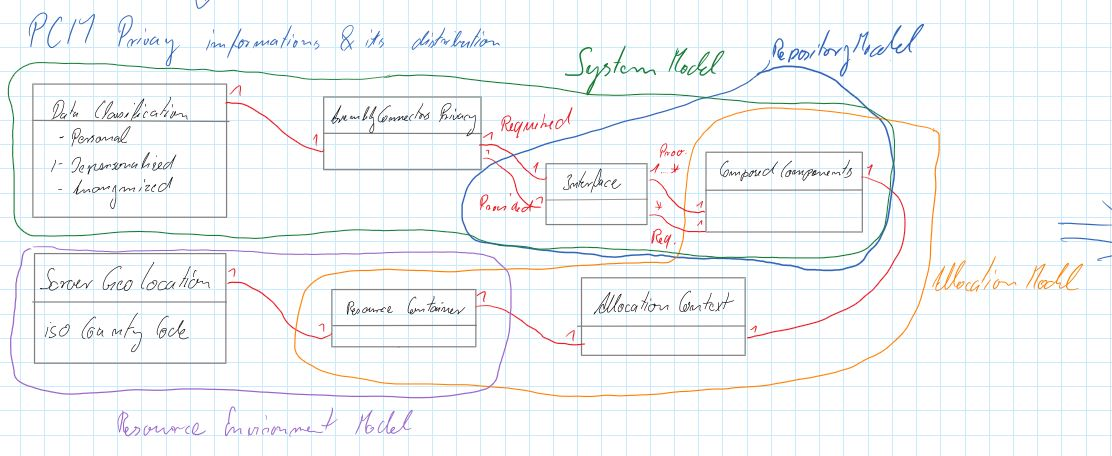
\includegraphics[width=0.5\textwidth]{pictures/pcm_info_spread}
	\caption{PCM Privacy information spread}
	\label{fig:pcm_info_spread}
\end{figure}

\begin{figure}[h]
	\centering
	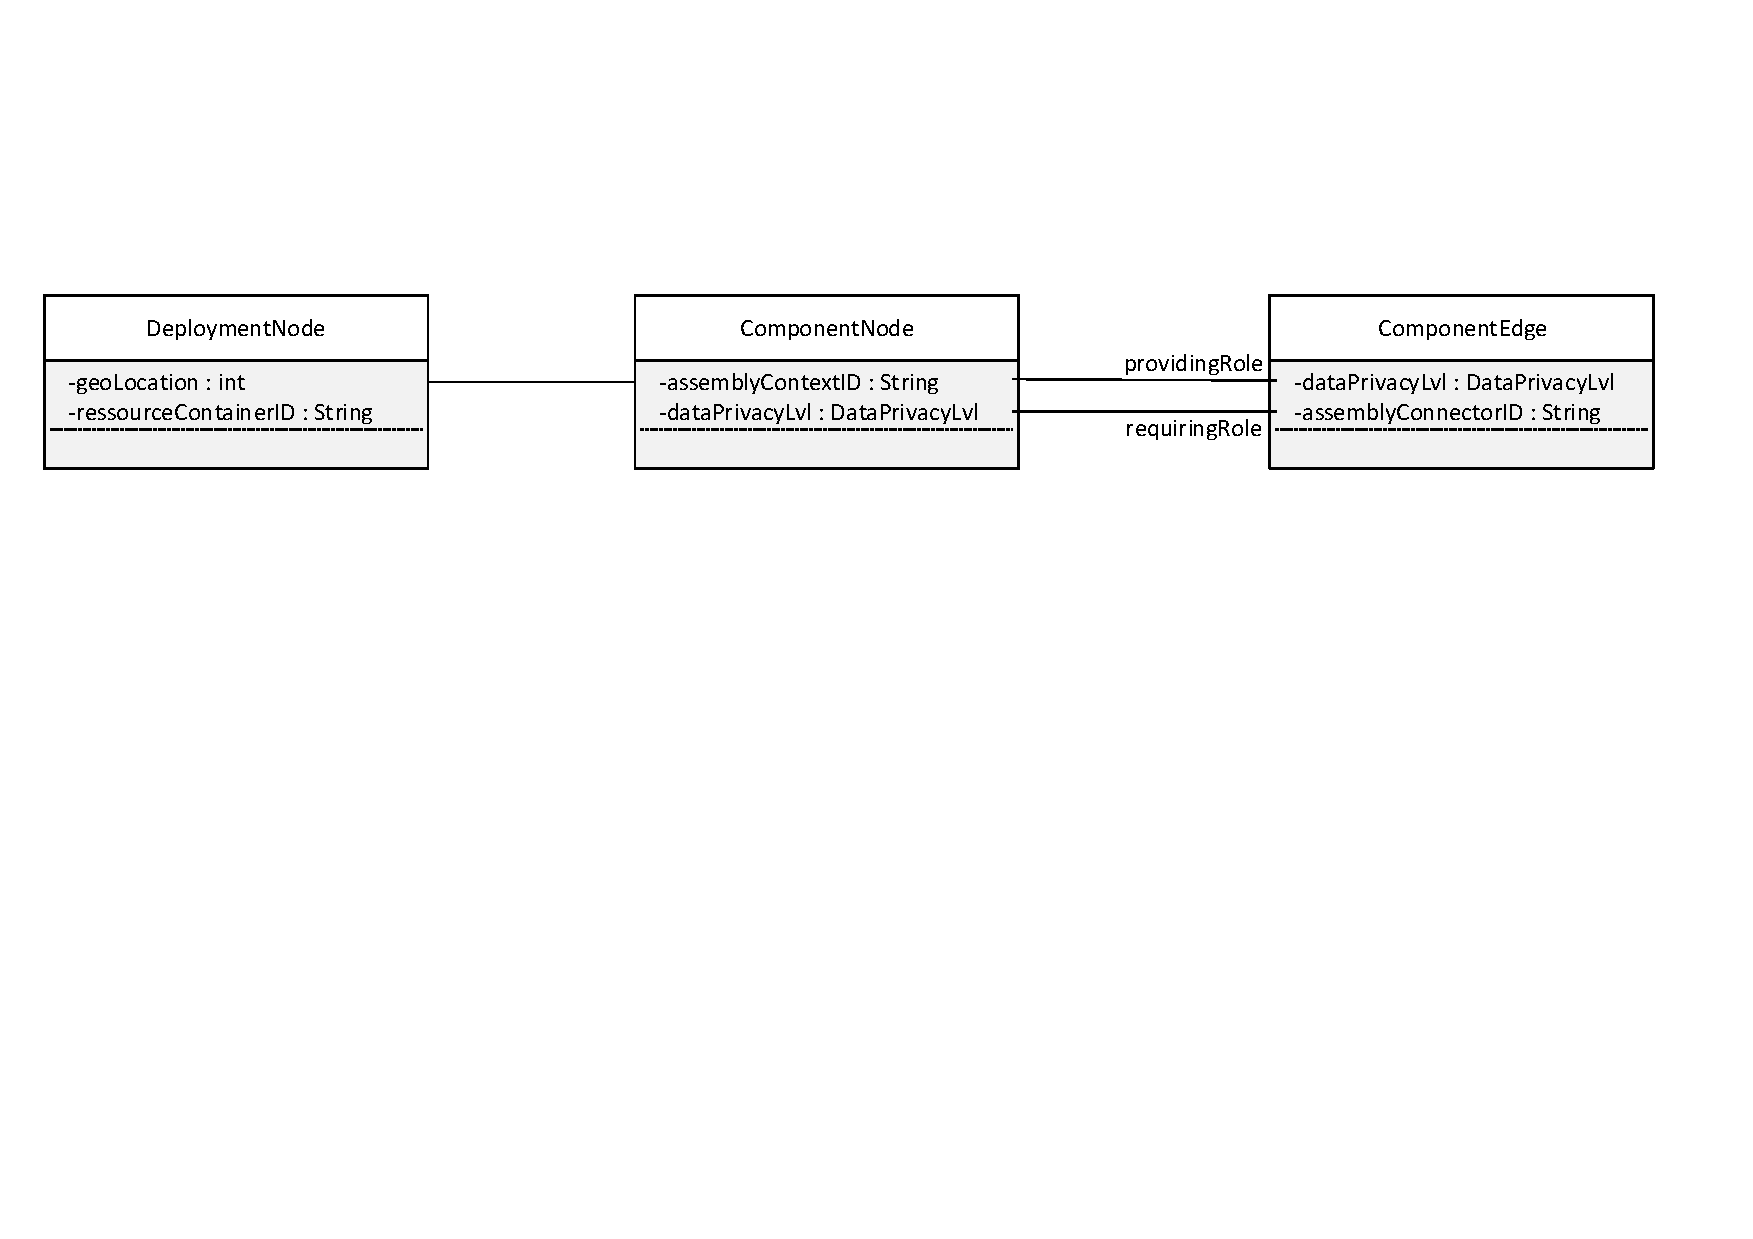
\includegraphics[trim = 00mm 120mm 15mm 50mm, clip, width=0.85\textwidth]{pictures/modelGraph_metamodel}
	\caption{Graphs meta-model for Privacy Analysis}
	\label{fig:privacy_graph_mm}
\end{figure}


\subsection{Component categorization implementation}

The second phase of the privacy analysis algorithm finalizes the component categorization. As described in \autoref{sec:PrivacyAnalysis:categorization}, joining data streams need to be found and fitting components' data privacy level corrected.

The algorithm (Algorithm \ref{algo:comp_categ}) searches for depersonalised-marked connections from one personal categorized component to another. It uses a \textit{deep search first} approach, while never using an edge twice. Note, that once a joining data stream is found, the involved components are appended to the list of personal components.

\begin{algorithm}[h]
	\caption{Component categorization algorithm}
	\label{algo:comp_categ}
\begin{algorithmic}[1]
	
	\State List of Components $components$
	\State Set of Edges $usedEdges$ 
	\State
	\Procedure{StartCategorization}{List<Components> $components$}\State
		$personalComponents\gets components with PrivacyLvl == PERSONAL$
		\ForAll{$personalComponent\gets Components$}\State
			\Call{clear}{ $usedEdges$ }\State
			\Call{TraverseComponent}{ $personalComponent$ }
		\EndFor
	\EndProcedure \State
	
	\Function{TraverseComponent}{Component $component$}\State
		$dePersonalEdges\gets component.$\Call{GetEdges}{} with $PrivacyLvl == DEPERSONAL$
		\ForAll{$edge\gets dePersonalEdges$}\State
			\If{$usedEdges.$\Call{Contains}{ $edge$ }} \State 
				\Call{Continue}{}
			\Else \State
				$usedEdges.$\Call{Add}{ $edge$ } \State
				$edgeParnter\gets edge.$\Call{GetEdgePartner}{ $component$ } \State
				
				\If {$edgeParnter.PrivacyLvl == PERSONAL$} \State
					\Return $edgeParnter$
				\Else \State
					$secondSource\gets$ \Call{TraverseComponent}{ $edgeParnter$ }
					\If{$secondSource \neq PERSONAL$} \State
						$component.PrivacyLvl\gets PERSONAL$ \State
						$components.$\Call{Add}{ $component$ } \State
						\Return $secondSource$
					\EndIf
				\EndIf 
			\EndIf
		\EndFor \State
		\Return Null
	\EndFunction
\end{algorithmic}
\end{algorithm}



\subsection{Deployment analysis implementation}

The final privacy analysis phase is the deployment evaluation. The base analysis is very simple, since it simply checks whether every as personal categorized component is deployed on an as save considered geo-location. The a geo-location is considered as save, when it is contained in the save-geo-location list. When a server is located in an un-save geo-location and contains more then one depersonalised component, an extensive analysis for joining data streams has to be made. This extensive analysis is described in Algorithm \autoref{algo:deployment_analysis}.

The Algorithm works similar to Algorithm \ref{algo:comp_categ}. Initially, it extracts all as depersonalised categorized components on the server. These components have to form a transitive hull and share a single depersonalised communication link to a single personal component. The algorithm uses a \textit{deep search first} approach to traverse through the components. If a second link to a personal component is found or not every depersonalised component on the server is reached, the deployment is illegal.

Note, that anonymized categorized components and edges can be ignored during analysis. Also, a server won't contain any personal marked component since such a deployment would be automatically illegal due to the servers un-save geo-location.


\begin{algorithm}[h]
	\caption{Deployment analysis algorithm}
	\label{algo:deployment_analysis}
	\begin{algorithmic}[1]
		
		\State Set of Components $compToReach$
		\State Set of Edges $usedEdges$
		\State Edge $dataSourceEdge$
		\State
		\Procedure{ExtensiveAnalysis}{Server $server$}
			\State $compToReach\gets server.$\Call{GetComponents}{} with $PrivacyLvl == DEPERSONAL$
			\State $dataSourceEdge \gets Null$
			\State $startComp\gets compToReach.$\Call{GetAny}{}
			\State {clear}{ $usedEdges$ }
			\State $singlePersonalDataSource\gets $\Call{TraverseComponent}{startComp}
			\State \Return $singlePersonalDataSource$ AND $compToReach.$\Call{IsEmpty}{} 
		\EndProcedure \State
		
		
		\Function{TraverseComponent}{Component $component$}
		\State $compToReach.$\Call{Remove}{ $component$ } 
		\State $dePersonalEdges\gets component.$\Call{GetEdges}{} with $PrivacyLvl == DEPERSONAL$\State
		
		\ForAll{$edge\gets dePersonalEdges$}
			\If{$usedEdges.$\Call{Contains}{ $edge$ }}
				\State \Call{Continue}{}
			\Else 
				\State $usedEdges.$\Call{Add}{ $edge$ } 
				\State $edgeParnter\gets edge.$\Call{GetEdgePartner}{ $component$ } 
				\State
				\If {$edgeParnter.PrivacyLvl == PERSONAL$}
					\If {$dataSourceEdge == Null$} 
					 	\State $dataSourceEdge \gets edge$
				 	\Else 
					 	\State \Return False
				 	\EndIf
				\Else \State
					$singleDataSource\gets$ \Call{TraverseComponent}{ $edgeParnter$ }
					\If{$singleDataSource$} 
						\State \Return False
					\EndIf
				\EndIf 
			\EndIf
		\EndFor 
		\State \Return True
		\EndFunction
	\end{algorithmic}
\end{algorithm}



\chapter{PerOpteryx Extension}
\label{ch:PerOpt}

PerOpteryx, briefly introduced in \autoref{sec:Foundations:peropteryx}, is a model optimization framework. It is designed to calculate performance and cost optimised PCM models. For this purpose PerOpetryx uses an evolutionary algorithm to generate new PCM candidates. PerOpteryx uses a \textit{Design Decisions} EMF model to create a \textit{Design Space}. The design space is defined via \textit{Degrees Of Freedom}. Every degree of freedom allows for a finite amount of \textit{Decisions}. A \textit{Candidate} consists of one choice per degree of freedom and represents a PCM instance. 

Every candidate needs to be evaluated in order to decide if the \textit{Decisions} made during its constructions lead to a good results. Each evaluator can produce multiple results per analysis run. Each result belongs to a certain \textit{QML dimension}. A dimension has \textit{Objectives} and/or \textit{Constraints}, which helps the evolutionary algorithm to find the Pareto-optimal candidates. Every evaluator is encapsulated in an \textit{Eclipse Plug-in} \cite{PerOpteryx.b}. Since we need another evaluator, we need to create a new plug-in.

\section{Plug-in Design}
\label{sec:PerOpt:design}

We want to provide a \textit{Privacy Analysis} evaluator for PerOpteryx, while using our previously developed \textit{Privacy Anylsis} (\autoref{ch:PrivacyAnalysis}). Since both systems are based on the Palladio Component Model, the privacy analysis itself can be used as described in \autoref{ch:PrivacyAnalysis}. However, PerOpteryx does not know a "Privacy Dimension", which is required, since every analysis result needs an according dimension. A new dimension is required, since using a pre-existent dimension - like the "cost dimension" - would undermine the evolutionary algorithms optimizations effort. The privacy analysis has a single result, which is a \textit{Constraint}. It states, that no privacy violation is permitted.

As mentioned before, we need to create a new \textit{QML Dimension}, the \textit{Privacy Dimension}, which is referenced in a \textit{QML Contract Type}. The contract type references all the evaluation dimensions. The \textit{QML Declaration} references the contract type and specifies the actual objectives and constraints for the dimensions. Further, it specifies a \textit{QML Profile}, which \textit{Usage Model} is used for the evaluation.


\section{PerOpteryx Modification}

PerOpteryx' prior structure considers every generated candidate to be valid, only with different runtime results. This is incorrect, when the privacy dimension is included. Only privacy compliant models are valid options. As a result, we can abort the evaluation of the current PCM model, if the privacy constraint is broken. However, this means we need to execute the privacy evaluation first, check if the constraint is broken, break the evaluation if the model is invalid and fill all other objectives and constraints with according values.

As mentioned above, every evaluation is encapsulated in an \textit{Eclipse Plug-in}. So, every evaluation is represented as \textit{Proxy Analysis} in PerOpteryx, who has no information on what evaluation he is actually currently executing. To save evaluation time and increase our search space, we need to execute the Privacy Analysis first, while not breaking the generic evaluation characteristic. As a result, the \textit{IAnalysis} interface for every evaluation was extended with a \textit{Evaluation Complexity} query, returning an Enum representing the analysis runtime duration. PerOpteryx was modified in a way, that analysis returning the value \textit{VERY\_SHORT} get executed first. The Privacy Analysis evaluator returns this value.

Further, PerOpteryx was modified, to output the \textit{most cost efficient} candidate once all evaluation iterations are completely executed. The cost criteria was chosen over performance due to PerOpteryx's tendency to spread the allocation over many server to optimize the performance. The cost optimal model tends to group components on servers, reducing the servers required and therefore saving money, while still having a decent performance.


 


\chapter{System Adaptation}
\label{ch:SysAdap}

In the system adaptation stage of the iObserve Privacy pipeline the current software system is modified to match the re-deployment PCM. This filer stage represents part of the planning and the complete execution phase of the MAPE loop (\autoref{sec:Foundations:mape}).

The remainder of this chapter is structured into adaptation planning and the actual adaptation execution. It closes with a look onto the implementation.


\section{Adaptation Planning}
\label{sec:SysAdap:plan}

The planning phases job is to calculate what actions are required to bring the observed software system into the state defined by the redeployment model. While the task is pretty clear, the available source of informations are quite uncertain.

There are multiple potential sources of information that can be used to calculate adaptation steps. For example the \textit{Design Decisions} file used and modified by PerOpteryx (\autoref{ch:PerOpt}). This file contains all choices made during generation of the redeployment model. These informations are a viable source for action computation, however create a strong dependency on PerOpteryx. This means, if PerOpteryx would be exchanged for another model optimization tool, the complete adaptation planning needs to be rewritten.

Another information source for the adaptation planning could be the close observation of the candidate calculation/generation. This could be achieved by logging decisions made by the evolutionary algorithm. When considering, that the starting point of an evolutionary algorithms is usually a given input, the modification steps could be traced and remodelled for the system adaptation. However, evolutionary algorithms usually don't take the shortest path onto their end result and also random mutations are an valid generation factor. This means, the results needs to be analysed and optimized, while also injecting observations probes. While being a good potential information source, the effort for post-generation analysis and the resulting dependencies make it a bad choice.

We decided to make a direct comparison of the runtime PCM and the redeployment PCM. This builds up no further dependencies and the shortest adaptation path can be found. However, the information preprocessing and the comparison algorithm can be more complex than the other options.

\subsection{Adaptation Actions}
Palladio models are independent from programming languages, technologies and other specifics. We decided to enforce this characteristic by defining technology independent actions. They contain the required information, without knowing anything about the used technologies.

Further, we designed a set of basic actions which allows us to transform any PCM into another. The actions can be grouped into two major disjunct subgroups: the \textit{Assembly Context Actions} and the \textit{Resource Container Actions}.

\begin{itemize}
	\label{enum:SysAdap:plan:actions}
	\setlength\itemsep{0em}
	\item \textbf{Assembly Context Actions}
	\begin{itemize}
		\setlength\itemsep{0em}
		\item Allocate Action
		\item Deallocate Action
		\item Migrate Action
		\item Change Repository Component Action
	\end{itemize}
	\item \textbf{Resource Container Actions}
	\begin{itemize}
		\setlength\itemsep{0em}
		\item Acquire Action
		\item Replicate Action
		\item Terminate Action
	\end{itemize}
\end{itemize}

Assembly Context Actions reflect all model changes around a software component. Allocate, Deallocate and Migration Actions are self explaining. The Change Repository Component Action addresses the possibility to exchange a software component with an equivalent one. This can due to better fitting performance characteristics, while required and provided interfaces stay the same. As a result, the structure of the system model stays unchanged, but an encapsulated component gets exchanged for another one.

Resource Container Actions reflect changes around a virtual or physical server. Acquire and Terminate Actions don't need any explanations. A Replicate Action clones a server instance with its containing components.

\subsection{Action Ordering}

After all required actions are determined, an order must be established. We decided for the most simple but effective approach: "acquire, migrate, terminate." Meaning, first acquire the new servers, change the component allocations and finally terminate the unnecessary servers. This way no component get moved onto non-existent servers.

\todo{add conditions for actions and generate universal order!}


\todo{More details and thought on ordering!}



\section{Adaptation Execution}
\label{sec:SysAdap:exec}

The adaptation execution is as straight forward as it gets. The actions get executed - in order determined by adaptation planning (\autoref{sec:SysAdap:plan}) - by calling equivalent scripts, which wrap the technological side of the action. The technological implications are not considered by this thesis and are therefore not further discussed.
\todo{Ref to Pöppke?}
\todo{More details, when scripts \& implementation are rdy?}



\section{Implementation}
\label{sec:SysAdap:impl}


The implementation is split into three parts: the action calculation, the action ordering and the action execution. The calculation is based on the same graph as used during the \textit{Privacy Analysis} (\autoref{fig:privacy_graph_mm}). The Assembly Context Actions get calculated independently from the Resource Container Actions, the principle however is the same:

\begin{algorithm}[h]
	\caption{Action Calculation algorithm}
	\label{algo:action_calc}
	\begin{algorithmic}[1]
		
		\State Dictionary $components$
		\State List of Action $actions$
		\State
		
		\Procedure{Init}{List<Components> $runtimeComponents$}
			\ForAll{$runComponent\gets runtimeComponents$}\State
			$components.$\Call{put}{$runComponent.AssemblyContextID$, $runComponent$ }
			\EndFor
		\EndProcedure
		\State
		\State
		\Procedure{CalculateActions}{List<Components> $reDeplComponents$}\State
			\ForAll{$reDeplComp\gets reDeplComponents$}\State
				$runComp\gets $ \Call{get}{$reDeplComp.AssemblyContextID$}
				
				\If {$runComp ==$ Null} \State
					$actions.$\Call{add}{ new $AllocateAction($\dots$)$ }
				\Else
					\If { $runComp.ComponentID$ != $reDeplComp.ComponentID$ }
						\State $actions.$\Call{add}{ new $ChangeRepoAction($\dots$)$ }
					\EndIf
					\If { $runComp.ResContainerID$ != $reDeplComp.ResContainerID$ }
						\State $actions.$\Call{add}{ new $MigrateAction($\dots$)$ }
					\EndIf
				\EndIf
				\State $components.$\Call{remove}{$reDeplComp.AssemblyContextID$}
			\EndFor
			\State
			\ForAll{$runComp\gets components$}
				\State $actions.$\Call{add}{ new $DeallocateAction($\dots$)$ }
			\EndFor
		\EndProcedure
	\end{algorithmic}
\end{algorithm}

Initially the algorithm adds all assembly components to a dictionary. In the main procedure, the algorithm iterates over all redeployment assembly components and tries to find a matching one in the runtime model. If no match as found, it is a new assembly component and needs to be allocated. If an equivalent was found, different comparison are made, to check whether adjustments have to made. Keep in mind, that the migration of a assembly component and the exchange of encapsulated repository component do not exclude each other. At the end of every iteration, the found runtime components get removed from the dictionary. At the end of the algorithm all remaining runtime assembly components are no longer required and can be deallocated. We need to point out, that the comparing operators are simplified for the purpose of a pseudo-code.

The calculation of the Resource Container Actions is implemented similar. Initially all servers get added to a dictionary, all redeployment servers get compared against those and the actions calculated accordingly.

The whole calculation is build around the stability of IDs on Palladio model elements. If the redeployment model creates a completely new system model, while changing only minor details, the calculation will deallocate the old system and allocate a totally new one. PerOpteryx modifies the system model, keeping the assembly context IDs - as intended - stable and therefore produces only minimal actions.

\todo{Check back with Replicate Action}

\todo{Describe Ordering}

\todo{Describe Execution}



%% LaTeX2e class for student theses
%% sections/evaluation.tex
%% 
%% Karlsruhe Institute of Technology
%% Institute for Program Structures and Data Organization
%% Chair for Software Design and Quality (SDQ)
%%
%% Dr.-Ing. Erik Burger
%% burger@kit.edu
%%
%% Version 1.3, 2016-12-29

\chapter{Evaluation}
\label{ch:Evaluation}

This chapter is structured as follows: Initially the concept is elaborated (\autoref{sec:Evaluation:concept}), followed by evaluation scenarios (\autoref{sec:Evaluation:scenarios}) and the evaluation of the single tasks: monitoring (\autoref{sec:Evaluation:monitoring}), privacy analysis (\autoref{sec:Evaluation:monitoring}), model generation (\autoref{sec:Evaluation:privacyanalysis}), adaptation planning (\autoref{sec:Evaluation:planning}) and finally adaptation execution (\autoref{sec:Evaluation:execution}).

\section{Evaluation Design}
\label{sec:Evaluation:concept}

iObserve Privacy is a complex approach with many depending tasks. Evaluating the program as a whole is next to impossible due to the multiplexing dependencies. The evaluation factors would not be manageable and inconclusive results would make the evaluation itself pointless. So we decided to evaluate every task independently. The order and structure got inspired by the iObserve pipeline.

%Accuracy => Scenarios => unbiased
The task evaluation is generally split into an \textit{Accuracy} evaluation and a \textit{Scalability} evaluation. The accuracy evaluation aims for the correct functionality, testing whether the actual results are conform to expected results. For the evaluation we are creating a set of \textit{Evaluation Scenarios}, which reflect real world situations by defining a staring point and an expected endpoint. If the systems result differs from the endpoint, the reasons must be found and analysed.

%Scalability => Runtime behaviour, automatic generated PCMs, 1 > 10 > 100 > 1000 ... logarithmic scale
The scalability evaluation aims for the systems runtime characteristic, based on an increasing work load. The actual accuracy result of the task doesn't interest during this analysis. The primary measurement is the task response time, dependent on the assembly context count and resource container count. Both axis are logarithmic scaled, so the response behaviour is clearly visible. The individual models are randomly generated, based on a repository model input.

\section{Evaluation Scenarios}
\label{sec:Evaluation:scenarios}

The scenarios are structured in \textit{PRE}, \textit{EVENT}, \textit{REACTION} and \textit{POST}. Pre describes the distributed software system before the event takes place. The event is a trigger for a certain process or task chain, usually referenced as reaction. Post defines the state of the software system after the reaction.

The scenarios describe the behaviour of iObserve Privacy through all tasks, while each task gets evaluated individually. Nevertheless, details of an scenario may need clarification during the evaluation of this task.

The scenarios are derived from \cite{Heinrich.2016b}. This paper describes potential runtime changes to a distributed software system. However, not all mentioned scenarios are of interest in the privacy analysis context. Scenarios 1 and 2 represent the observed system runtime changes. However, major iOberve privacy failing scenarios are not covered. This is due to the iObserve Privacy design specific nature of error states. Scenario 3 and 4 cover these error.

\subsection{Scenario 1: Default}
\label{eval:scenario:1}
% PRE: Amazon Deployment @ EU WEST
% CASE: Critical Error => Amazon moves instances to EU WEST & US EAST
% POST: Migration Monitored, Privacy Analysis started
%					=> IF OK:	Do nothing 
%					=> IF BAD:	Calculate Alternative (Privacy Compliant) => Plan => Adapt => Evaluate!
This scenario describes the "default" setting. A migration gets monitored, analysed, an alternative deployment calculated and finally migrated. The process works completely automated. This means no operator interaction is required and no task error is generated. As trigger for privacy analysis the server geo-location migration is used.
\begin{itemize}
	\setlength\itemsep{0em}
	\item \textbf{PRE}: All components of the software system are deployed on Amazons EC2 service on the \textit{EU Frankfurt} location. The system is privacy compliant.
	\item \textbf{EVENT}: Amazons EU Frankfurt data centre has a critical failure. As a result Amazon starts migrating local virtual machines towards the US Ohio and EU Ireland locations.
	\item \textbf{REACTION}: iObserve Privacy monitors the migration and starts a privacy analysis. If the analysis doesn't show a privacy violation no further action is taken. If the analysis shows a privacy violation, an alternative, privacy compliant deployment gets computed, a system adaptation plan gets calculated and finally executed.
	\item \textbf{POST}: The software system is in a privacy compliant state.
\end{itemize}


\subsection{Scenario 2: System extension}
\label{eval:scenario:2}
% PRE: 	Privacy components @ Microsoft; Non-Privacy @ UKRAINE
% CASE:	New DePersonalized Component gets deployed @ UKRAINE
% POST: Deployment Monitored => Privacy Analysis started => "Joining Data Streams" found => Calculate Alternative (Privacy Compliant) => Plan => Adapt => Evaluate!

This scenario describes the deployment runtime change. The deployment of a new software component triggers a privacy analysis, which detects "joining data streams" (see \autoref{sec:PrivacyAnalysis:theory}). This triggers the generation of an alternative deployment and the system adaptation. The pipeline works like in Scenario 1 without any operator interaction.
\begin{itemize}
	\setlength\itemsep{0em}
	\item \textbf{PRE}: All personal categorized components of the software system are deployed on Amazons EC2 service on the \textit{EU Frankfurt} location. All other components are hosted by an Ukrainian provider. The system is privacy compliant.
	\item \textbf{EVENT}: The system operator adds another as depersonalised categorized component to the Ukrainian host.
	\item \textbf{REACTION}: iObserve Privacy monitors the migration and starts a privacy analysis. The privacy analysis shows a privacy violation due to joining data streams. An alternative, privacy compliant deployment gets computed, a system adaptation plan gets calculated and finally executed.
	\item \textbf{POST}: The software system is in a privacy compliant state.
\end{itemize}

\subsection{Scenario 3: Failing Adaptation}
\label{eval:scenario:3}
% PRE: 	All @ Cheap Hoster (Europe SLA)
% CASE:	Some components migrate @ UKRAINE
% POST: Deployment Monitored => Privacy Analysis started => Privacy Violation found => Calculate Alternative (Privacy Compliant) => Plan => Adapt can't be done automatically => Call the Operator
This scenario describes the operator-in-the-loop use case, when an adaptation sequence can't be executed automatically. The migration of a software component results in a privacy violating state. After the generation of a privacy compliant alternative and the calculation of the adaptation sequence, the operator is required. One or more adaptation actions can't be executed automatically. This is usually due to missing source control, like the \textit{Change Repository Component Action} or the \textit{Allocation Action}.
\begin{itemize}
	\setlength\itemsep{0em}
	\item \textbf{PRE}: All components of the software system are hosted multiple server instances by cloud reseller. 
	\item \textbf{EVENT}: The reseller starts migrating his server to another cloud providers.
	\item \textbf{REACTION}: iObserve Privacy monitors the migration and starts a privacy analysis. The privacy analysis shows a privacy violation. An alternative, privacy compliant deployment gets computed. The adaptation calculation shows certain steps can't be executed automatically. After ordering the adaptation steps the operator gets informed for manual execution.
	\item \textbf{POST}: iObserve Privacy shows the operator the adaptation sequence with emphasis on the manual tasks.
\end{itemize}


\subsection{Scenario 4: Missing Alternative}
\label{eval:scenario:4}
% PRE: 	All @ Cheap Hoster (Europe SLA)
% CASE:	Some components migrate @ UKRAINE
% POST: Deployment Monitored => Privacy Analysis started => Privacy Violation found => Calculate Alternative (Privacy Compliant) => No Privacy Compliant Alternative Found => Call Operator
This scenario describes the use case, where no privacy compliant, alternative deployment could be calculated. The migration of a software components results in a privacy violating state. The calculation of privacy compliant alternatives deployment fails. The operator needs to be informed about the current situation.
\begin{itemize}
	\setlength\itemsep{0em}
	\item \textbf{PRE}: All components of the software system are hosted multiple server instances by cloud reseller. 
	\item \textbf{EVENT}: The reseller starts migrating his server to another cloud providers.
	\item \textbf{REACTION}: iObserve Privacy monitors the migration and starts a privacy analysis. The privacy analysis shows a privacy violation. An alternative, privacy compliant deployment can't be computed.
	\item \textbf{POST}: \dots
	\todo{Specify end state!}
\end{itemize}

%\subsection{Scenario 5}
% PRE: 	Privacy components @ Amazone EU WEST; Non-Privacy @ Cheap Hoster (Europe SLA)
% CASE:	Cheap Hoster constantly migrates to the cheapest hoster => Moves two Depersonal instances to the same server in Ukraine
% POST: Migration Monitored, Privacy Analysis started
%			=> "Joining Data Streams" found => Calculate Alternative (Privacy Compliant) => Plan => Adapt => Evaluate!

\subsection{Futile Scenario}
There are a couple of scenarios which don't apply to iObserve Privacy, due to various reasons \cite{Heinrich.2016b}. We will elaborate those scenarios shortly.

%Performance
Performance or workload characteristics are not tackled, since performance and privacy analysis combined wouldn't be manageable in the scope of this thesis.

%Undeployment
The un-deployment or de-replication are two scenarios which reduce the complexity of the privacy analysis. A privacy violation can't be triggered by eliminating a component and/or a server from the system.

%Replication
The replication of a server, with all its components, will trigger a deployment event. This means, this scenario is already covered by \textit{Scenario 2}.


\section{Evaluation Models}
\label{sec:Evaluation:models}

In the previous sections we defined a couple of scenarios for the evaluation. In order to execute these scenarios, we need PCM Privacy models (\autoref{ch:pcmExtension}). Scenario and model need to get selected individually, depending on task to evaluate.

\subsection{CoCOME-Cloud}
\label{sec:eval:models:cocome}

The \textit{CoCOME Cloud} PCM model is a representation of the CoCOME system as a distributed cloud variant. It is a representation of a supermarket IT infrastructure. It exists of six individual deployed components:  \textit{logic.webservice.cashdeskline.cashdeskservice}, \textit{Cloud.Web}, \textit{traidingsystem.inventory}, \textit{traidingsystem.cashdeskline}, \textit{webservice.inventory} and \textit{traidingsystem.external.bank}. The system is oriented on real systems with dozens of interfaces and multiple composite components. As a result, CoCOME-Cloud is very complex and not suited for the evaluation of specific aspects. However, it is as the only available model fully specified and "PerOpteryx ready". See \cite{Heinrich.2015} for detailed information on CoCOME.


\subsection{Medi System}
\label{sec:eval:models:medSys}

\begin{figure}[h]
	\centering
	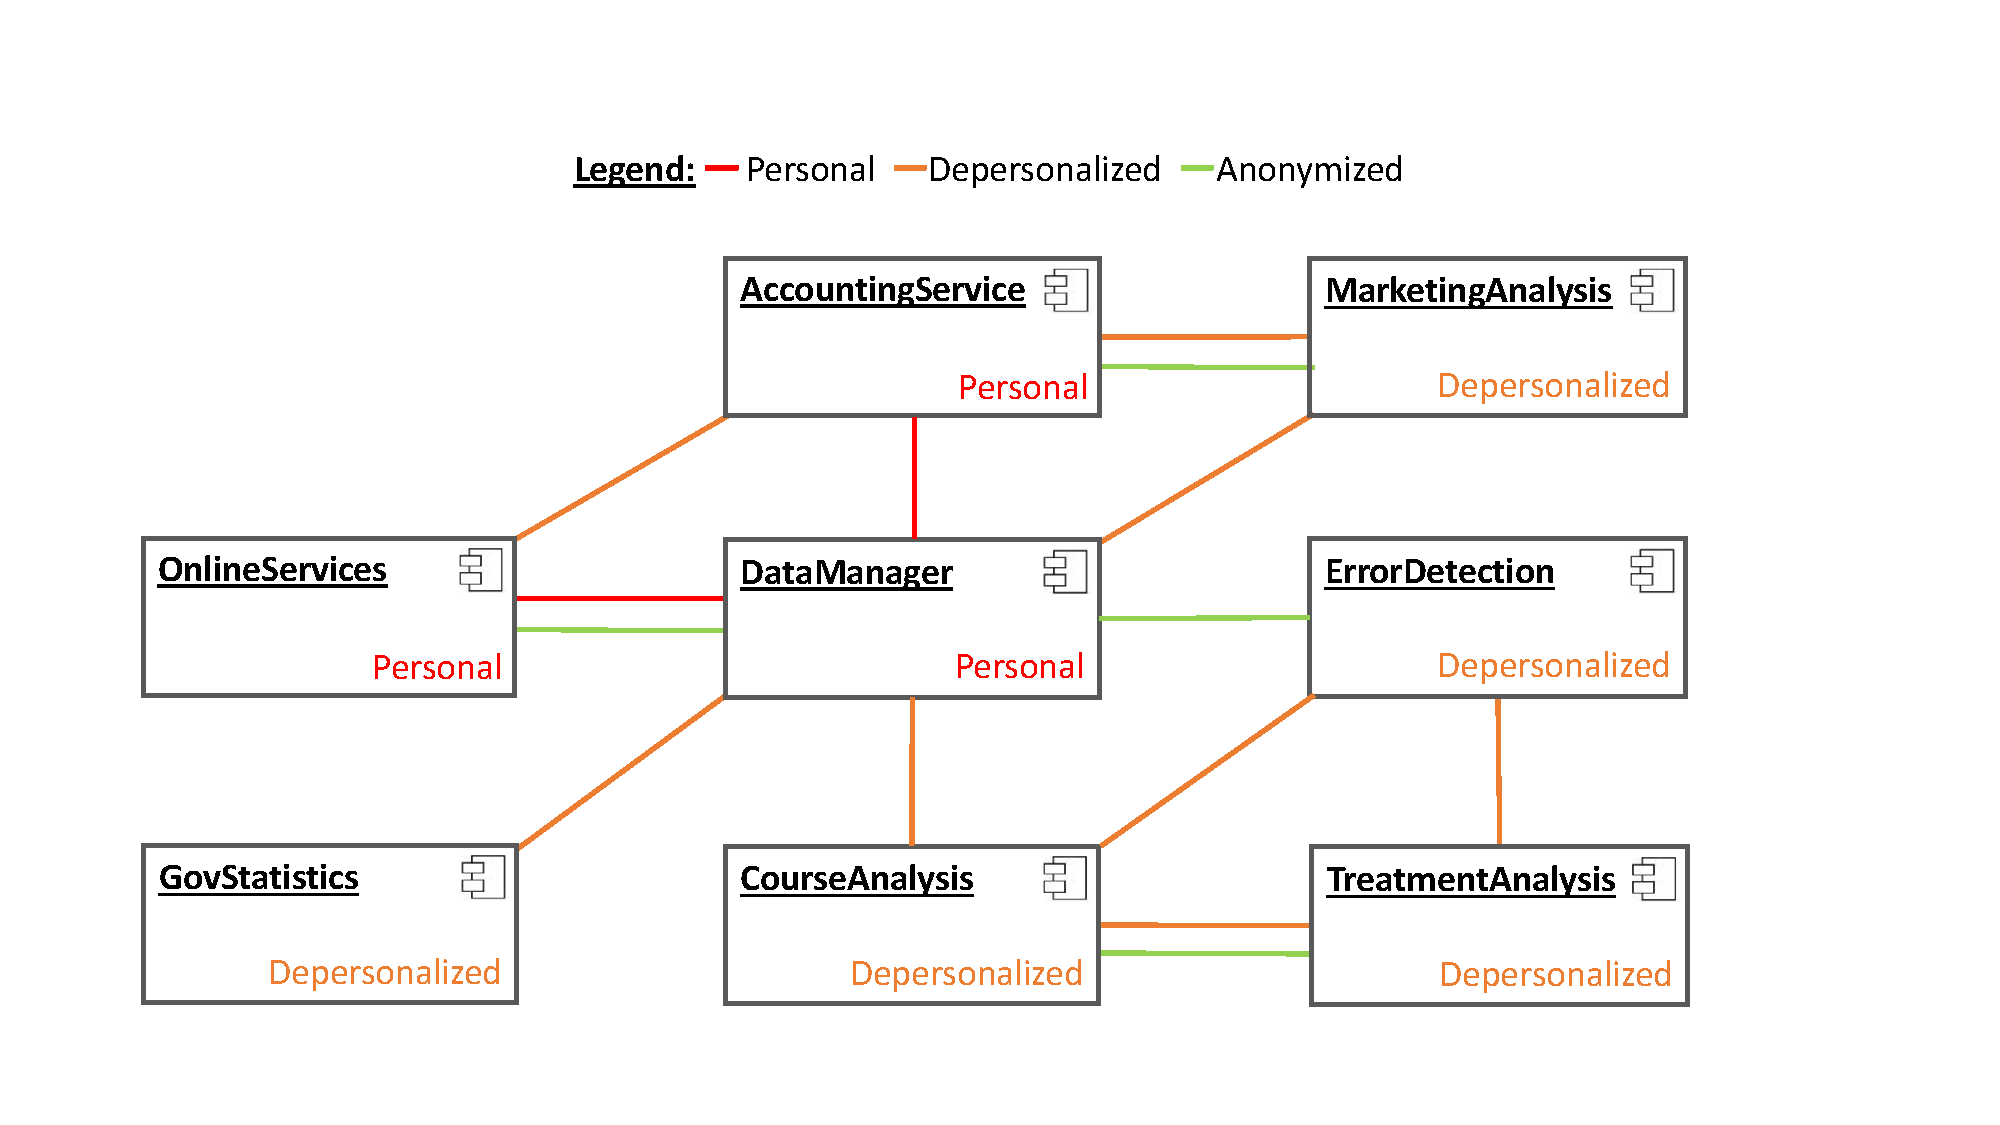
\includegraphics[trim = 0mm 10mm 0mm 20mm, clip, width=0.90\textwidth]{graphs/medSystem_noserver}
	\caption{Initial component categorization}
	\label{fig:model:medi}
\end{figure}

The \textit{Medi System} is an PCM model, specially developed for the evaluation of this thesis. It is supposed to reflect the web system of a medical insurance. The required and provided interfaces are reduced to the minimal necessary, to limit side effects and to gain meaningful results. \autoref{fig:model:medi} shows the medi system with all components and interface connections. The deployment will depend on the evaluation scenario.


\subsection{Generated Models}
\label{sec:Evaluation:models:generated}

We developed a model generator and model modificator for the scalability analysis. The generator requires an input repository and creates a valid PCM Privacy model with the given amount of assembly contexts and resource container. The contained component in the assembly context is randomly selected, as well as the resource container it is allocated on. All required interfaces are correctly connected, primarily to provided interfaces without an existing connection. The privacy categorization of an Assembly Connector Privacy is randomly chosen with a distribution of 15\% Personal, 35\% Depersonalised and 50\% Anonymized.

The model modificator adapts the system randomly, based on action counts specified. The modification supports server acquisition and termination and assembly context allocation, deallocation and migration. Further it supports the exchange of the contained repository component for a component with the same interfaces. Note, the generated models are only suited for the scalability analysis. 



\section{Transformation}
\label{sec:Evaluation:monitoring}

The Transformation evaluation aims for an accuracy and scalability test of the pipeline trigger events and the actual transformation of the send information onto the model. \textit{Scenario \#1} (\autoref{eval:scenario:1}) and \textit{Scenario \#2} (\autoref{eval:scenario:2}) describe the two possible triggers: the \textit{TDeployment Event}, when a component got deployed on a server, and the \textit{TGeoLocation Event}, when the geo-location of a server changes. 

\subsection{Transformation: Accuracy Evaluation}

For the accuracy evaluation we are using the CoCOME-Cloud model (\autoref{sec:eval:models:cocome}), since it is completely specified and reflects the a real system the best way available. We need to show, that the TDeployment Event and the TGeoLocation Event process the according data correctly and transform the send data correctly onto the model. Potential errors must be handled and avoided. This will show, that the problem and research question in \autoref{sec:Introduction:problems} was successfully solved.

In the first run, we will start with an empty, allocation model and use only valid data:

\begin{table}[h]
	\centering
	\begin{tabular}{r | l}
		\hline
		\textbf{Action} & \textbf{Values}\\
		\hline
		Deployment & tradingsystem.external.Bank on Server6-EU\\
		Deployment & tradingsystem.cashdeskline on Server4-EU\\
		Deployment & cloud.web on Server1-EU\\
		Deployment & webservice.inventory on Server1-EU\\
		Deployment & tradingsystem.inventory on Server2-EU\\
		Deployment & logic.webservice.cashdeskline.cashdeskservice on Server3-EU\\
		GeoLocation & Server1-EU on 276 (GER)\\
		GeoLocation & Server2-EU on 276 (GER)\\
		GeoLocation & Server3-EU on 250 (FRA)\\
		GeoLocation & Server4-EU on 250 (FRA)\\
		GeoLocation & Server5-EU on 826 (GBR)\\
		GeoLocation & Server6-EU on 826 (GBR)\\
		UnDeployment & cloud.web from Server1-EU\\
		Deployment & cloud.web on Server1-NonEU\\
		GeoLocation & Server4-EU on 804 (UKR)\\
		\hline
		\end{tabular}
	\caption{The correct execution set}
	\label{tab:valid_run}
\end{table}

We expect a run without any errors, an allocation model, which represents the described deployment and a design decisions model, which the according degree of freedoms.

The results are unbiased. The system reports no errors and the models represent the system exactly as intended.

To test the robustness, we need to input invalid events on a logical level. To gain a valid system state, we are starting with the valid order (\autoref{tab:valid_run}) and append illegal orders. We expect these orders to give a warning and to be ignored. The system must continue running. The test includes the following cases: Deployment of already deployed components, deployment of an undeployed component on a non-existing server, geo-location record from a non-existing server, un-deployment of a non-existing deployment. Illegal arguments are marked with a *:

\begin{table}[h]
	\centering
	\begin{tabular}{r | l}
		\hline
		\textbf{Action} & \textbf{Values}\\
		\hline
		Deployment & cloud.web on Server1-EU*\\
		UnDeployment & cloud.web from Server1-NonEU\\
		UnDeployment & cloud.web from Server1-NonEU*\\
		Deployment & cloud.web on Server7-EU*\\
		Deployment & IllegalComonent on Server1-EU*\\
		UnDeployment & IllegalComonent from Server1-EU*\\
		UnDeployment & tradingsystem.inventory from Server2-NonEU*\\
		GeoLocation & Server7-EU on 826 (GBR)*\\
		\hline
	\end{tabular}
	\caption{The error execution set}
	\label{tab:error_run}
\end{table}

The error run shows ends up to be exactly as intended, with one exception. The UnDeployment event \textit{tradingsystem.inventory from Server2-NonEU*} is executed and the component is un-deployed even though is placed on Server2-EU instead of Server2-NonEU. This is due to a bug during allocation context retrieving. Due to a wrong output, when reading the resource container from the allocation context, the comparison of resource containers is deactivated. The bug has a random nature and could not be resolved. The current workaround has only this one side effete: the un-deployment of a component is executed, even if the given server does not match the actual allocation.


\subsection{Transformation: Scalability Evaluation}

For the scalability analysis we are using the Medi-System model with a generated Dat-File. The inputs are logically and syntax valid. 30\% of the inputs are TDeployment and TUnDeployment events, distributed relative to the current allocation status. The other 70\% of inputs are TGeolocation events, randomly distributed over all available servers. Every measurement was repeated three times to eliminate potential measurement errors. The log outputs remain active, the snapshot creation is deactivated, so no further pipeline filters get activated. The results (\autoref{fig:eval:runtime:transformation}) show a linear runtime behaviour, maximal input size is $1,oE06$ events.

\begin{figure}[h]
	\centering
	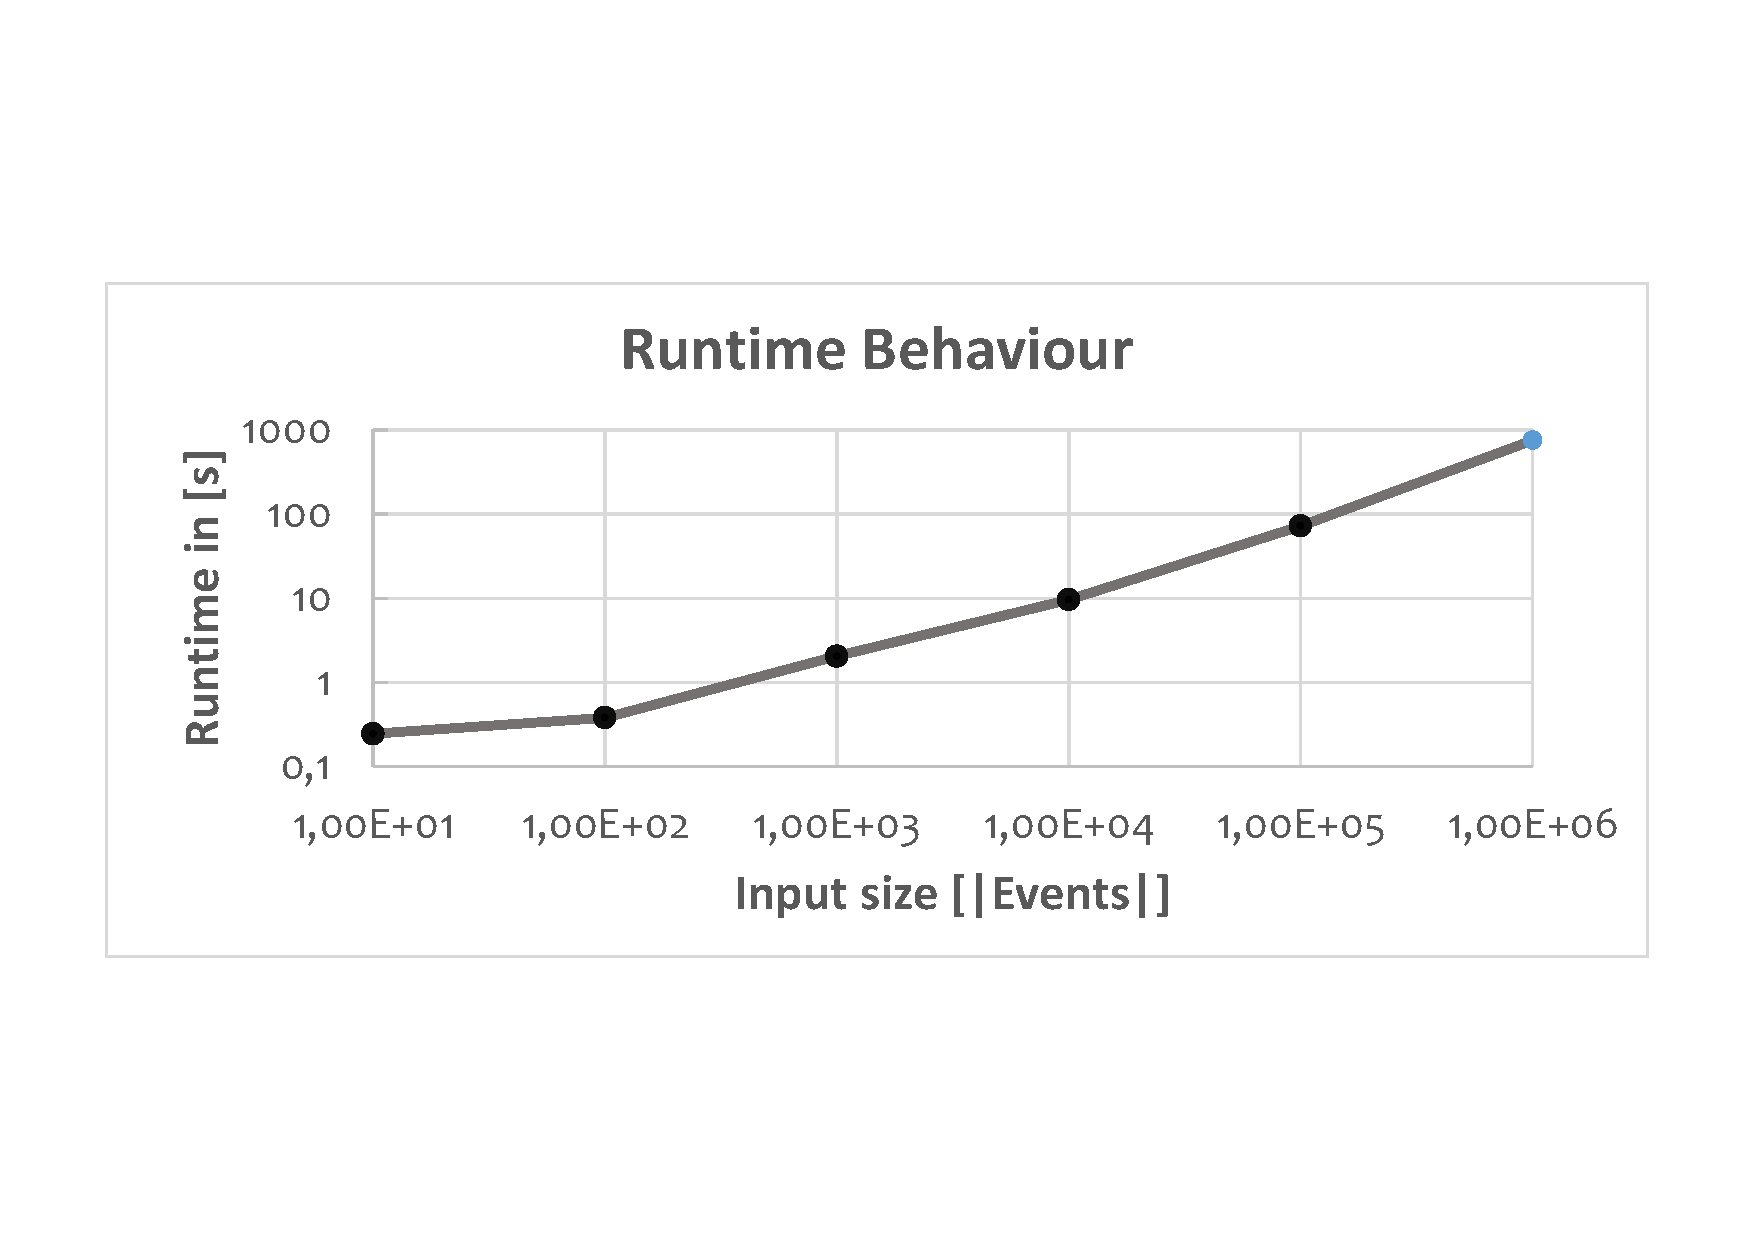
\includegraphics[trim = 0mm 40mm 0mm 40mm, clip, width=0.90\textwidth]{graphs/Runtime_Transformation}
	\caption{Runtime behaviour}
	\label{fig:eval:runtime:transformation}
\end{figure}


\section{Privacy Analysis}
\label{sec:Evaluation:privacyanalysis}

The \textit{Privacy Analysis} was extensively discussed in \autoref{ch:PrivacyConcept} (Privacy Concept) and \autoref{ch:PrivacyAnalysis} (Privacy Analysis). As described there, the privacy analysis consists of two sequential parts: \textit{Component Classification} and \textit{Deployment Analysis}. According to this tasks, the accuracy evaluation is also split. The accuracy evaluation uses the Medi-System model (\autoref{sec:eval:models:medSys}), due to its moderate complexity level, where effects like the \textit{Joining Data Stream} occurs, but the results are still traceable.

\subsection{Privacy Analysis: Accuracy Evaluation}

We will show, that the component classification categorizes components correctly, by finding \textit{joining data streams} in inter component communication. Further, we will show, that the deployment analysis finds \textit{joining data streams} on the deployment level. As a result, we demonstrate the correctness of our privacy analysis, as specified in the goal section (\autoref{sec:Introduction:goals}).

The scenarios \#1 (\autoref{eval:scenario:1}) and \#2 (\autoref{eval:scenario:1}) aim to trigger a privacy analysis. We showed in \autoref{sec:Evaluation:monitoring}, that both trigger, the TDeployment Event and the TGeoLocation Event are correctly processed and the information transformed onto the PCM model. Both trigger start the same privacy analysis and are therefore equivalent. 

\begin{figure}[h]
	\centering
	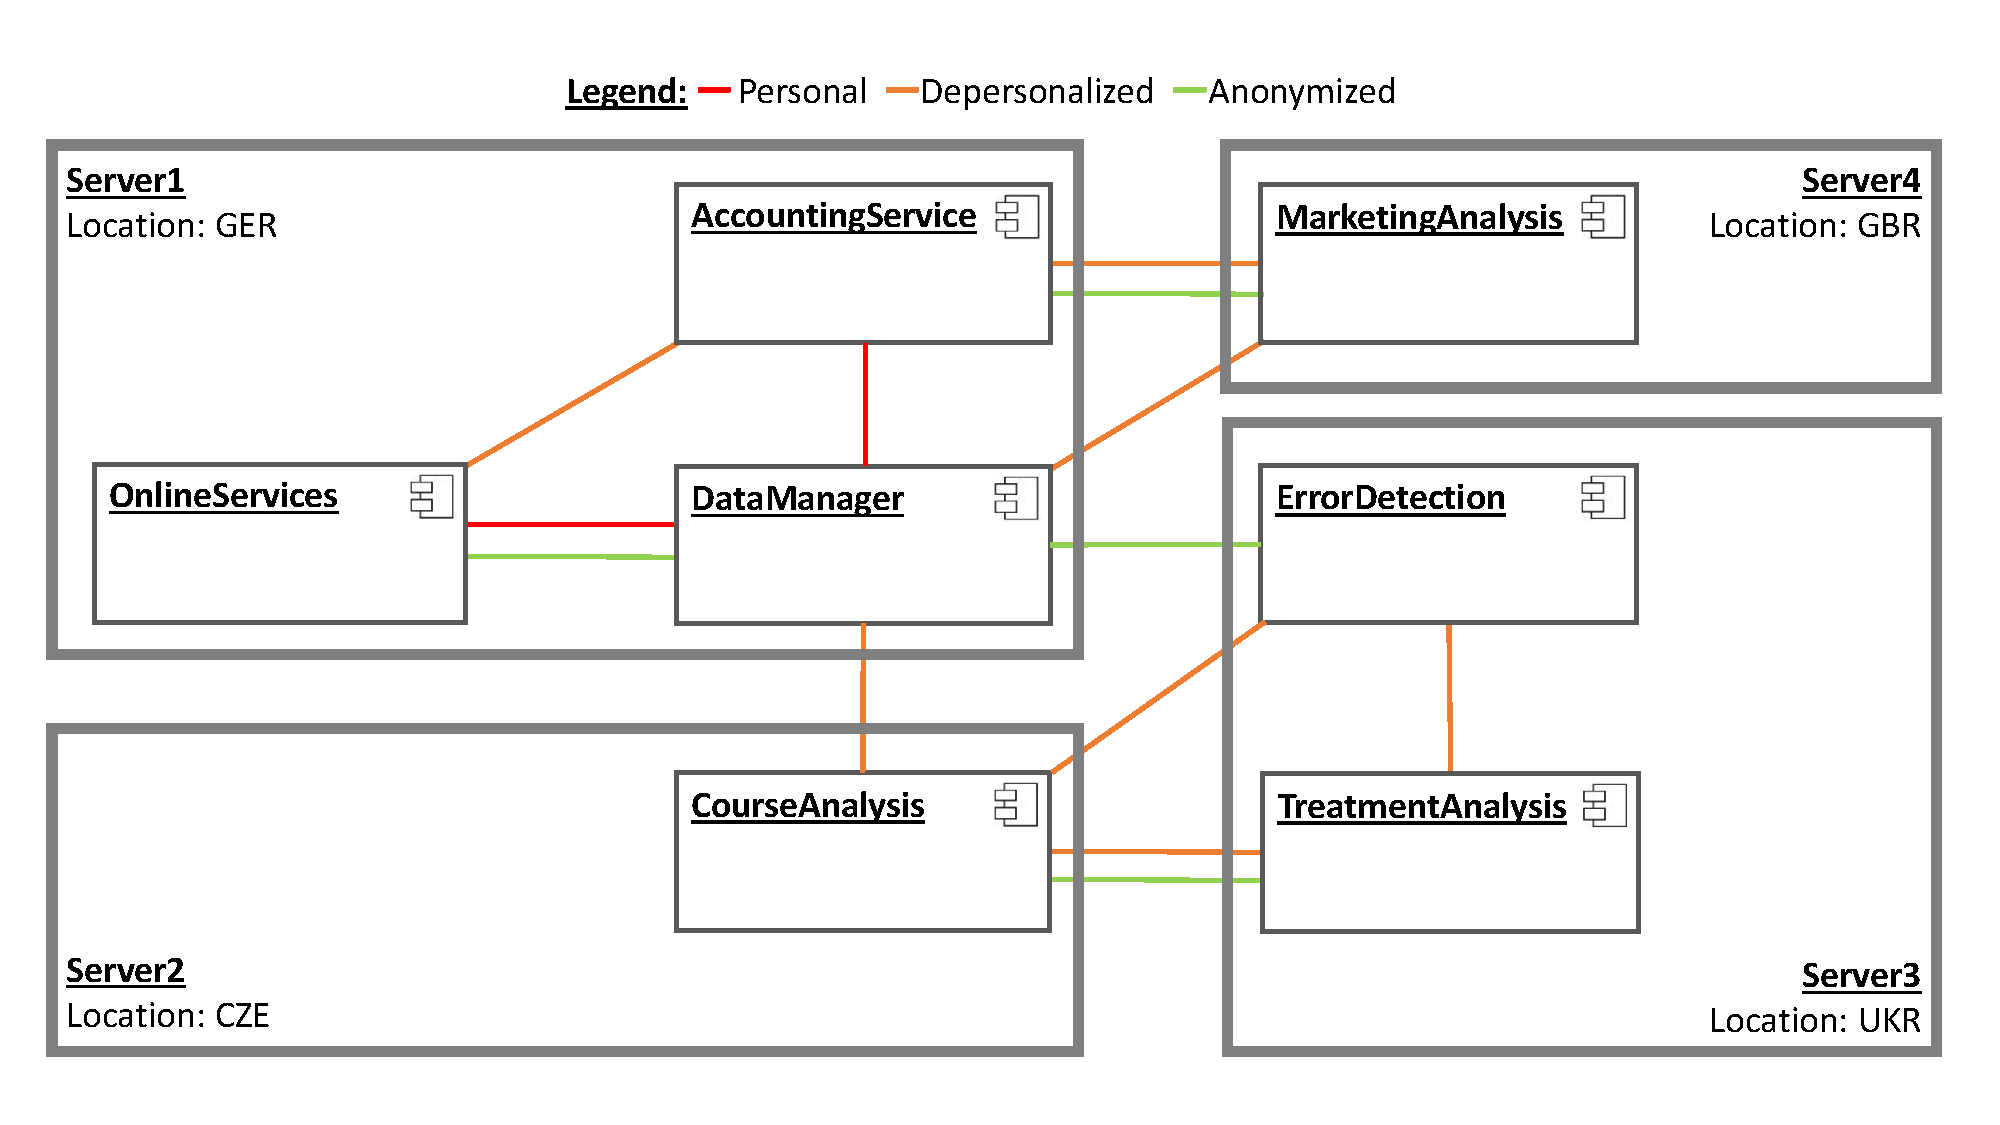
\includegraphics[trim = 0mm 10mm 0mm 10mm, clip, width=0.75\textwidth]{graphs/medSys_eval_pa_init}
	\caption{Initial system state}
	\label{fig:eval:pa:init}
\end{figure}

The initial system state is as show in \autoref{fig:eval:pa:init}. The system is privacy compliant and only the \textit{GovStatistics} component is not allocated onto a server. iObserve will trigger the pipeline by receiving a GeoLocation event, which migrates the \textit{Server2} to Belarus. We expect the initial component categorization to be equal to the most personal interface level the component has. After the \textit{Categorization Analysis} the \textit{MarketingAnalysis} component should be classified as personal, due to its two personal communication partners. The components \textit{ErrorDetection}, \textit{TreatmentAnalysis} and \textit{CourseAnalysis} data privacy level should remain unchanged, since they share a single depersonalised interface as data sources. The deployment must remain legal.

As a second trigger, we deploy the GovStatistics component onto Server2. The component must be tagged depersonalised and the deployment analysis must report a \textit{joining data stream} on Server2.

The result is \textit{unbiased}. The \autoref{fig:eval:pa:base_tag} shows the initial component categorization. \autoref{fig:eval:pa:categorized} shows the categorization analysis result. Both states fulfil the expectations. The deployment analysis reports a legal deployment.

\begin{figure}[h]
	\centering
	\begin{minipage}[b]{0.48\textwidth}		
		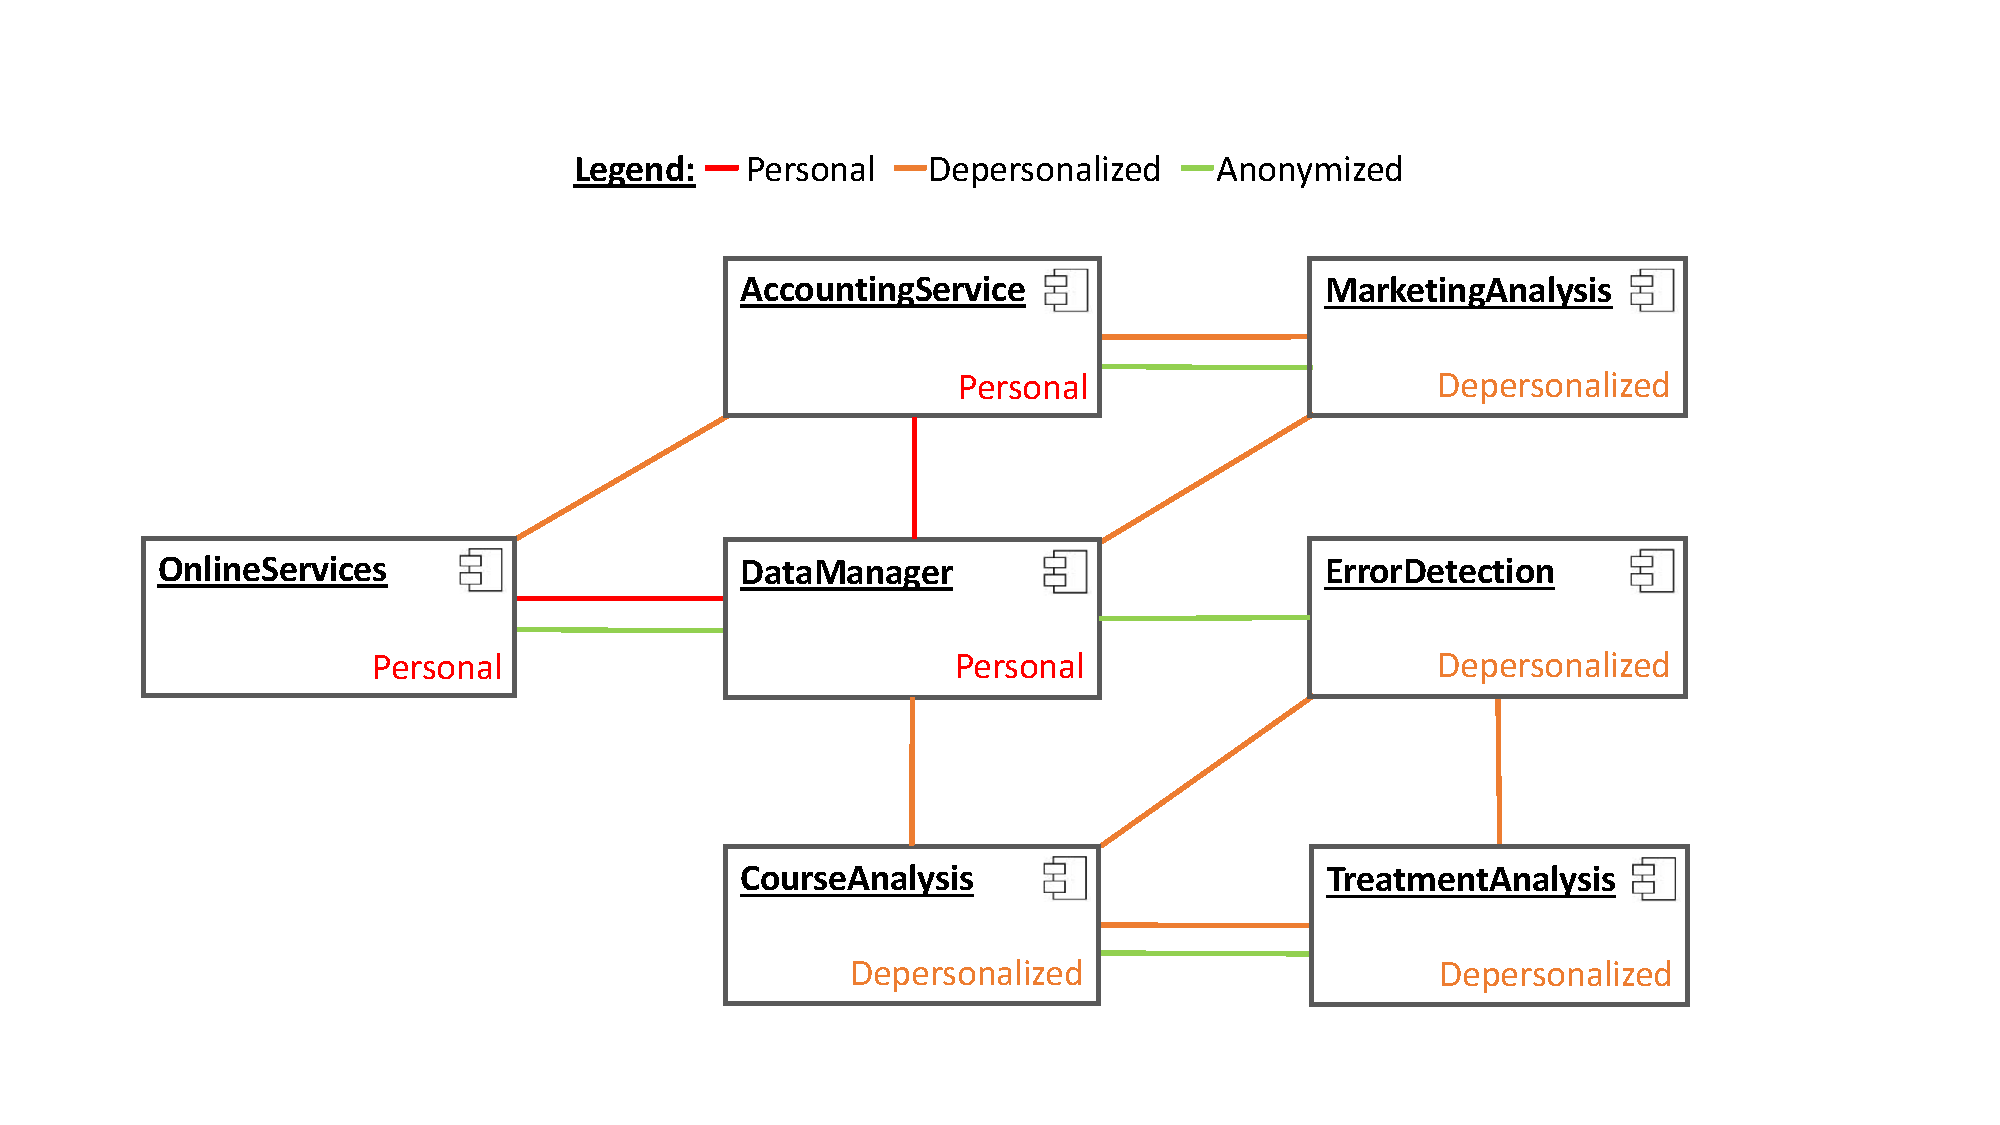
\includegraphics[trim = 20mm 10mm 40mm 10mm, clip, width=0.99\textwidth]{graphs/medSys_eval_pa_tagging_init}
		\caption{Initial categorization}
		\label{fig:eval:pa:base_tag}
	\end{minipage}
	\begin{minipage}[b]{0.48\textwidth}
		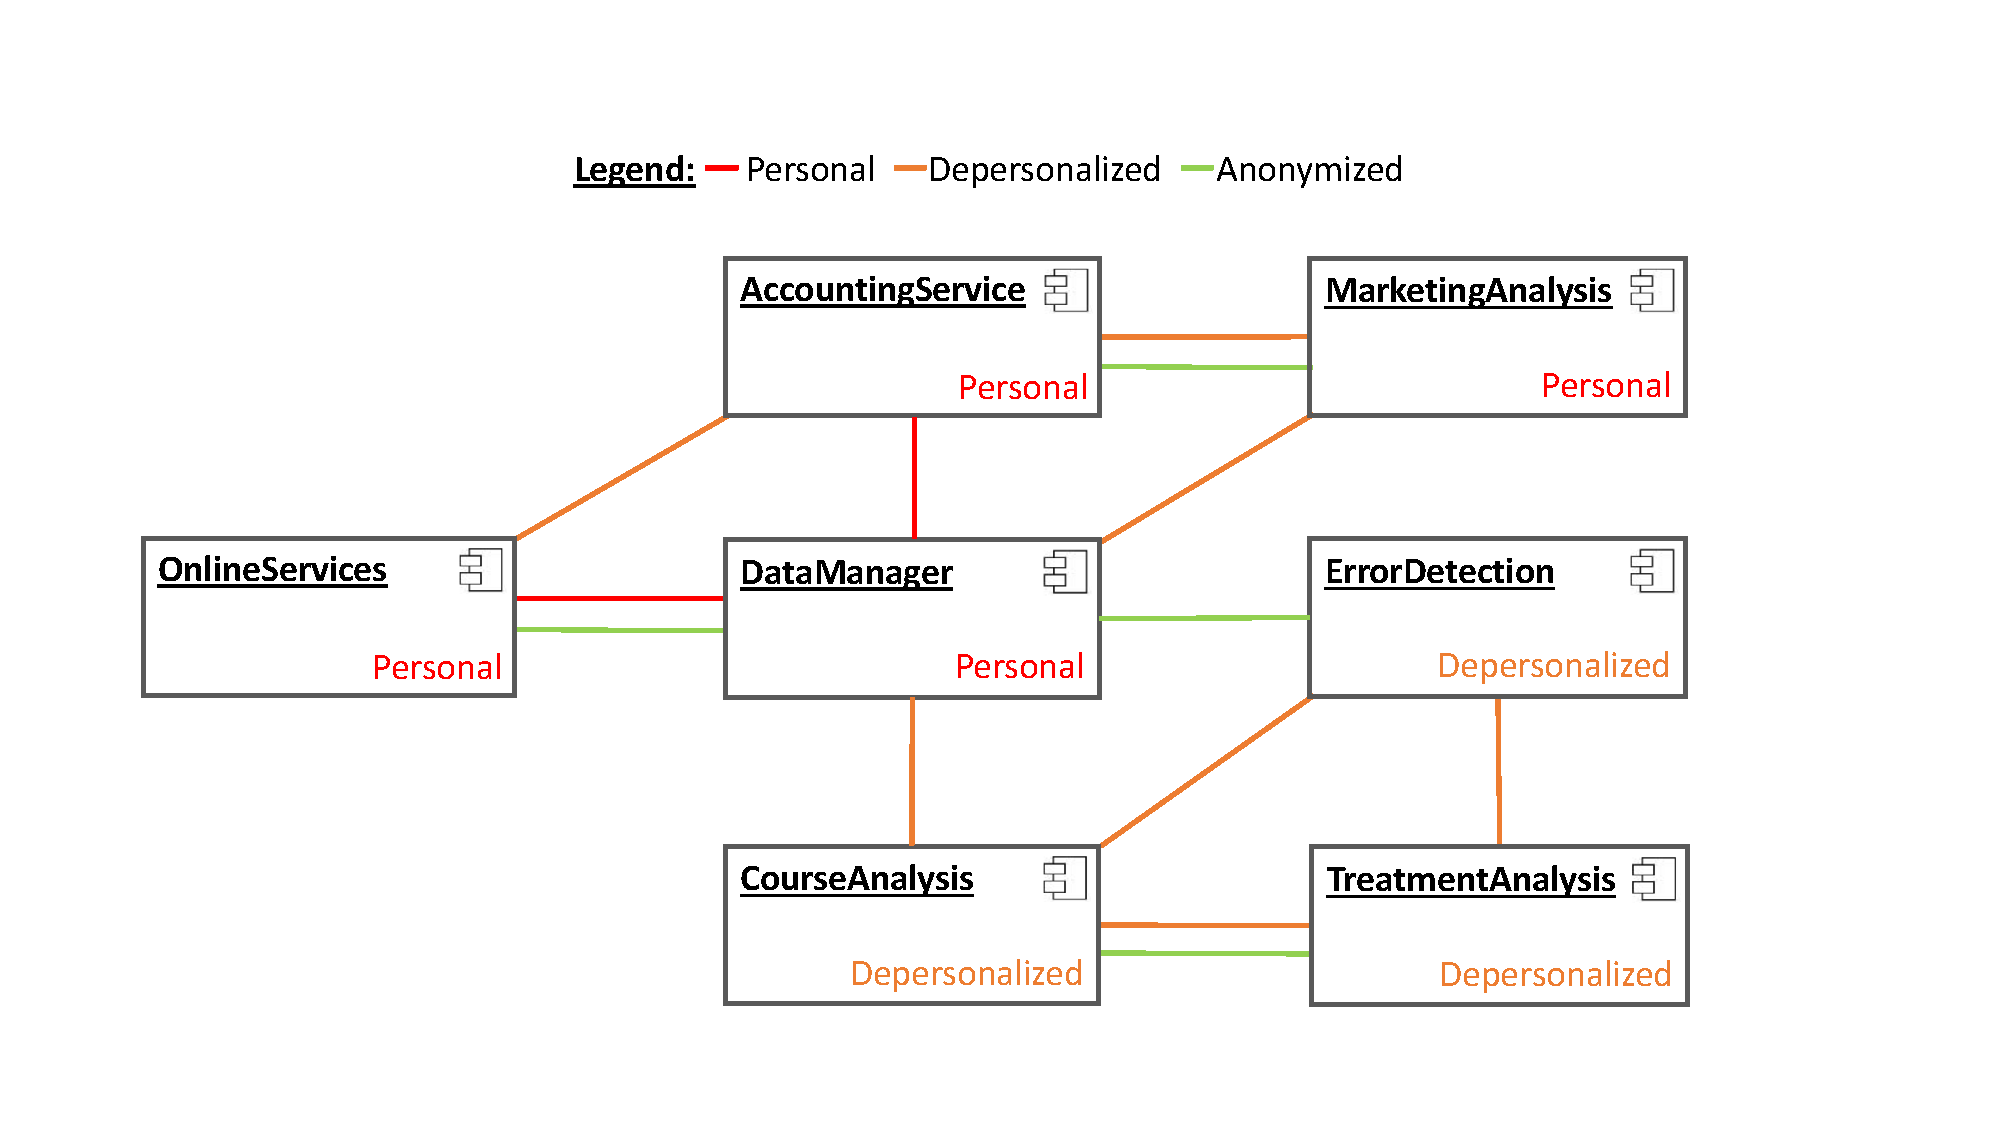
\includegraphics[trim = 20mm 10mm 40mm 10mm, clip, width=0.99\textwidth]{graphs/medSys_eval_pa_tagging_analysis}
		\caption{Categorization analysis result}
		\label{fig:eval:pa:categorized}
	\end{minipage}
\end{figure}

The second trigger, the component deployment on \textit{Server2}, reports a privacy violation. The cause is a joining data stream on Server2. This is what we provoked and expected.

\begin{figure}[h]
	\centering
	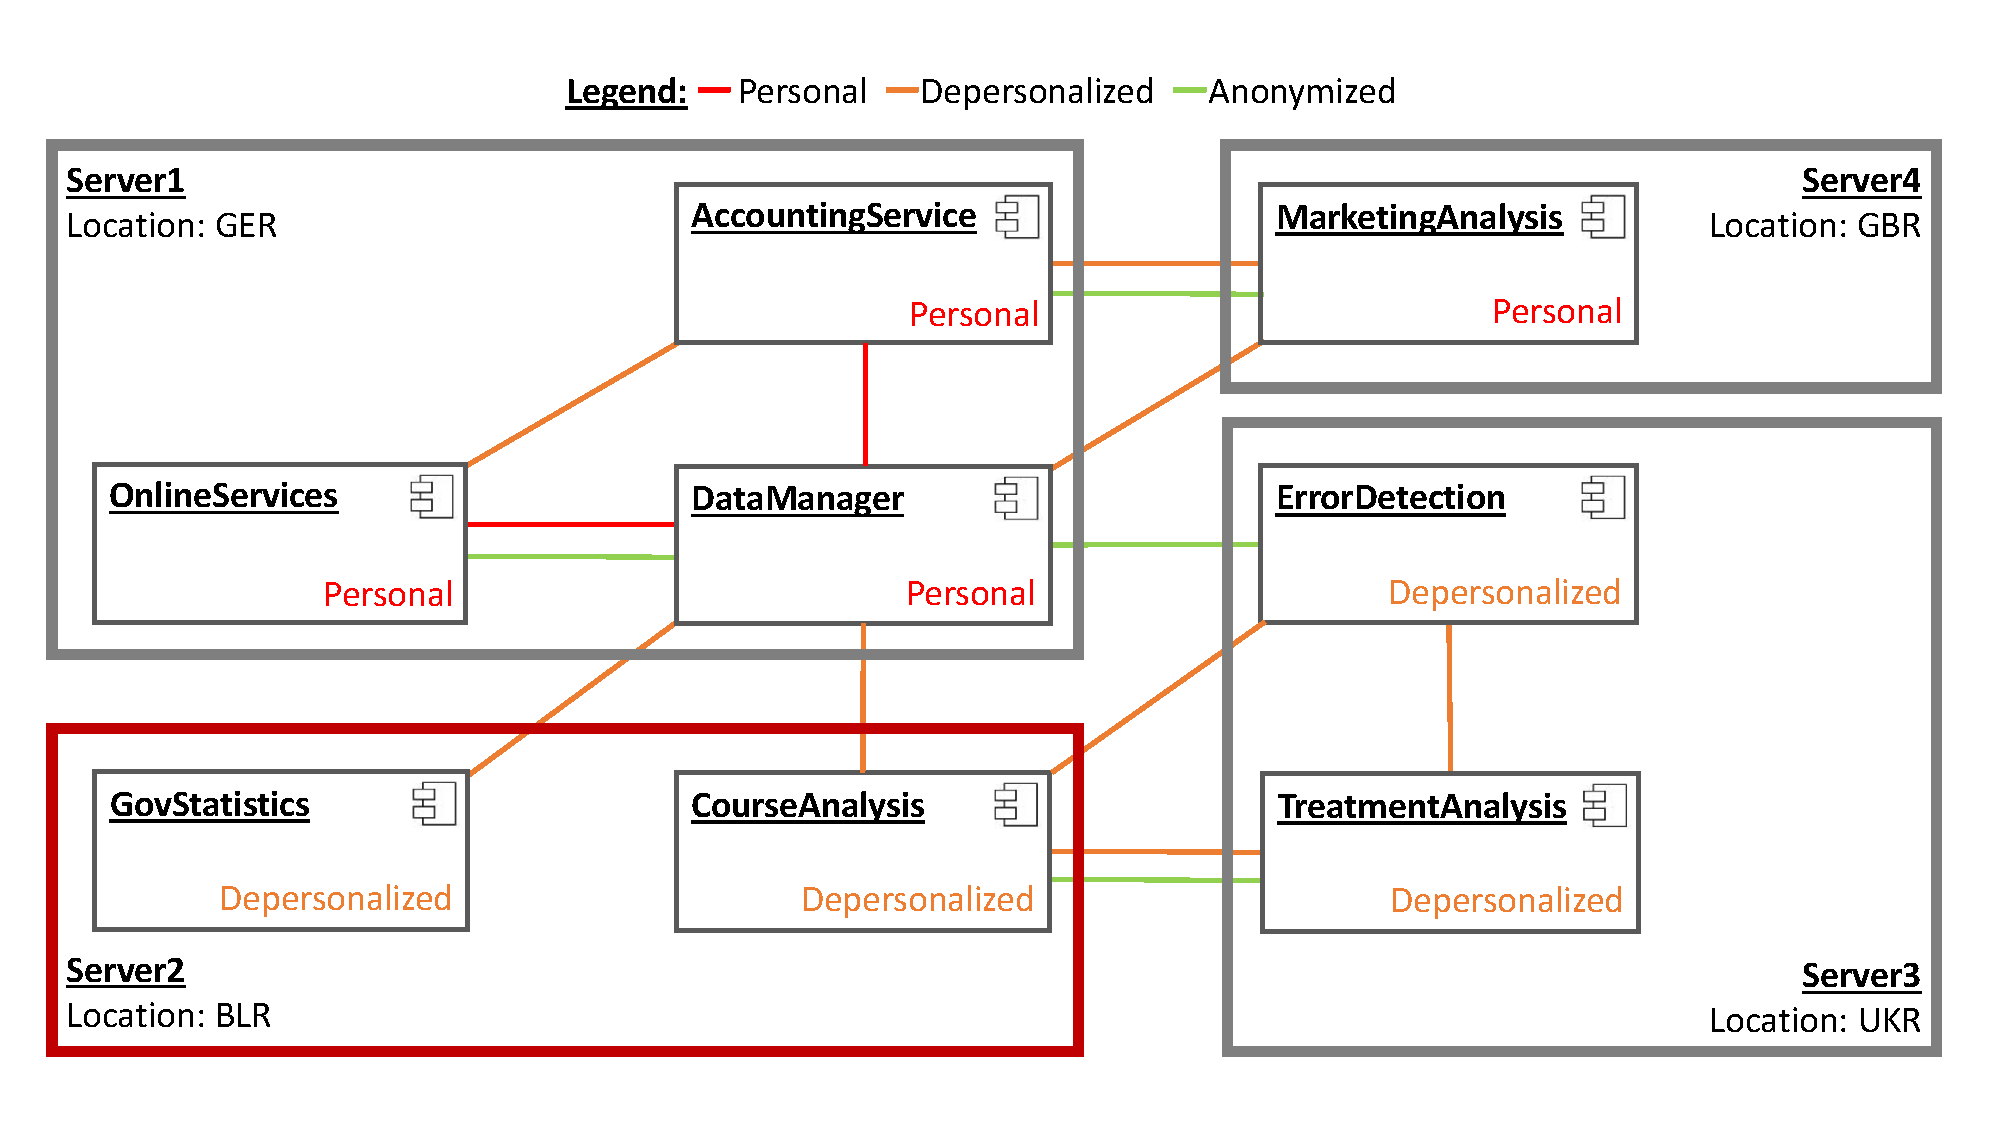
\includegraphics[trim = 0mm 10mm 0mm 10mm, clip, width=0.75\textwidth]{graphs/medSys_eval_pa_da}
	\caption{Deployment analysis result}
	\label{fig:eval:pa:depl_ana}
\end{figure}

We have shown, that the component classification algorithm and the deployment analysis works as intended, providing a privacy analysis on a architectural level (see \autoref{sec:Introduction:goals}). We didn't show every possible privacy violation, however showed the most difficult analysis work: The detection of joining data streams on component categorization and deployment analysis level. And the correct identification of a set of components, located on a server, sharing the same single depersonalised component as a data source. We will use further exemplary privacy violations in the other accuracy evaluations.

\subsection{Privacy Analysis: Scalability Evaluation}

For the scalability evaluation of the privacy analysis, we will use the generated model (\autoref{sec:Evaluation:models:generated}), since models of the intended evaluation scale are not constructable by hand. 


\section{Model Generation}
\label{sec:Evaluation:generation}

\dots

\section{Adaptation Planning}
\label{sec:Evaluation:planning}

\dots

\section{Adaptation Execution}
\label{sec:Evaluation:execution}

\dots
%%%%%%%%%%%%%%%%%%%%%%%%%%%%%%%%%%%%%%%%%%%%%%%%%%%%%%%%%%%%%%%%%%%%%%
\chapter{Related Work}
\label{ch:RelatedWork}

In this chapter we are presenting a couple of related publications, this work can be referenced to. The sections are oriented on the task and problems mentioned in \autoref{sec:Introduction:goals}.


\section{Application Monitoring}
\label{sec:RelatedWork:appl_mon}

The monitoring of software systems is common task in many research fields. Automated data-flow analysis, software profiling and hardware utilization are only a small selection of groups, using this term. In the following, we use application monitoring in the sense of online extraction of runtime data form a (distributed cloud) application for architecture optimization.

R-PRIS (\autoref{sec:RelatedWork:privacyanalysis}) and Kieker are application monitoring frameworks. While iObserve uses Kieker to extract the desired information, R-PRIS is independent from other programs. Neither of them uses a meaningful architecture description language (ADL) to process and store the gathered information. iObserve however gathers the transmitted data, processes them and stores them into a PCM model, enabling all kind of PCM-based applications to use the gathered information \cite{kieker.web}\cite{Schmieders.}\cite{Heinrich.2016}.


\section{Privacy Analysis}
\label{sec:RelatedWork:privacyanalysis}

R-PRIS is a monitoring and analysing tool for distributed cloud systems. Like iObserve, R-PRIS updates a runtime model by monitoring the cloud systems. During the analysis phase the model is checked for (potential) privacy violations.

Like Kieker, R-PRIS combines push-based heartbeat monitoring with event processing, and graph grammars for efficiently updating those models \cite{Schmieders.}. R-PRIS uses a formal specification for geo-location policies. These consists of data classification $S$, data content types $T$ and geo-locations $L$. Every specified policy $p = (S, T, L)$ is forbidden. This means, a data modelling is required with a \textit{Classification} and the containing \textit{ContentType} (see \autoref{fig:rpris_metamodel}). During privacy analysis R-PRIS checks whether a privacy protected information can be accessed from an non-privacy compliant location. This can be transformed into an st-connectivity problem, a standard problem in graph theory and analysis. Based on the runtime model (\autoref{fig:rpris_model}) - with its meta-model (\autoref{fig:rpris_metamodel}) - R-PRIS performs a reachability check \cite{Schmieders.2015}. 

\begin{figure}[h]
	\centering
	\begin{minipage}[b]{0.48\textwidth}		
		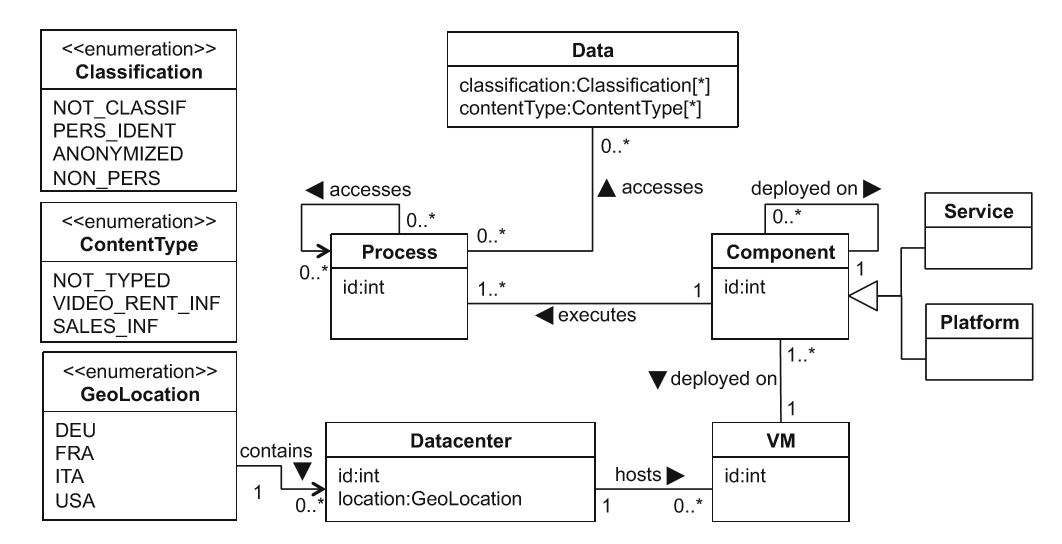
\includegraphics[width=\textwidth]{pictures/rpris_metamodel.jpg}
		\caption{R-PRIS meta-model}
		\label{fig:rpris_metamodel}
	\end{minipage}
	\begin{minipage}[b]{0.48\textwidth}
		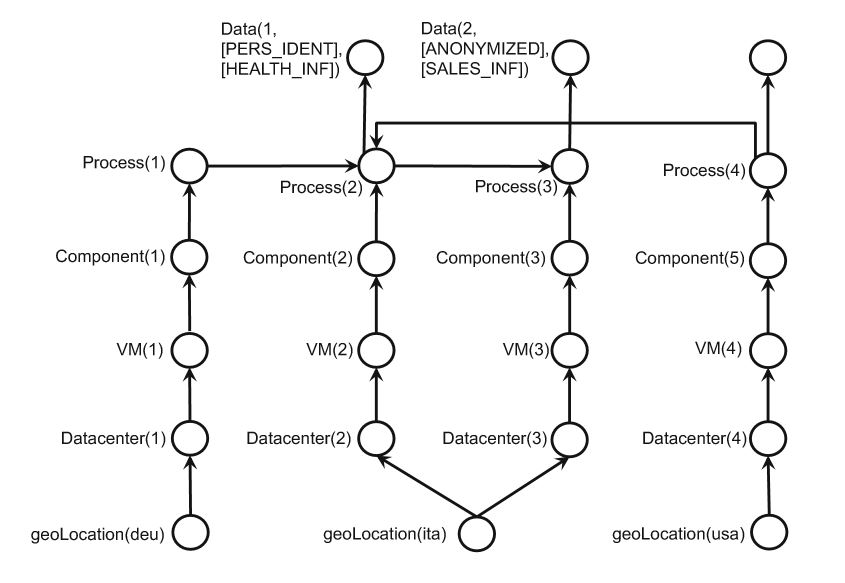
\includegraphics[width=\textwidth]{pictures/rpris_model.jpg}
		\caption{R-PRIS runtime model}
		\label{fig:rpris_model}
	\end{minipage}
\end{figure}

In terms of software, R-PRIS searches for communication paths in the distributed system, which can potentially transmit personal data to a non-privacy compliant geo-location. In order to detect these communication paths a policy $p$ must be specified, representing exactly this case, which however doesn't necessarily communicate private data. As a result, a lot of policies have to be specified, which prohibit many potentially harmless communication paths.

Based on their runtime model, Schmieders et al. identified four relevant migration-cases and extracted six required informations to detect a policy violation\cite{Schmieders.2015}:

\begin{table}[h]
	\centering
	\begin{tabular}{r | l}
		\hline
		\textbf{\#} & \textbf{Required information to carry out runtime check}\\
		\hline
		R1 & Interactions of two components\\
		R2 & Access of components to locally stored files\\
		R3 & Meta-information of stored or processed data\\
		R4 & Information on component deployments on physical resources \\
		R5 & Geo-location information of physical resources\\
		R6 & Explicit or implicit information on transitive data transfers\\
		\hline
	\end{tabular}
	\caption{R-PRIS information for runtime privacy checks \cite{Schmieders.2015}}
	\label{tab:rpris_information}
\end{table}


Due to the comparable core task of detecting privacy violations, we are comparing the R-PRIS privacy analysis against the iObserve Privacy privacy analysis. More detailed information on R-PRIS can be found in \cite{Schmieders.}\cite{Schmieders.2015}.

\begin{description}
	\item[Runtime Model] R-PRIS uses the specially developed model shown in \autoref{fig:rpris_metamodel}. Even while it models components, VMs and process, it does not capture the systems architecture as the Palladio Component Model does. Further, it is not known, whether tool support or other compatible programs exist, like the PCM has. 
\end{description}

\begin{description}
	\item[Categorization] We are utilizing a component communication classification, which leads to a component classification and a deployment analysis. Therefore, we do not know what data are actually processed in a component or on a server. R-PRIS, however, tags the data itself, traces the transitive access and prohibits rule violating access. As a result, R-PRIS, uses the more accurate \textit{data tracking}, which requires more information then and a deep knowledge about the observed system then iObserve privacy. While iObserve privacy uses data categorization by hand, the R-PRIS approach does not explain their modelling and categorization process.
\end{description}

\begin{description}
	\item[Rule Compliance] iObserve Privacy is clearly build to stay EU General Data Protection Regulation and HIPAA compliant. Therefore, a simple file input with \textit{save} geo-locations is sufficient. R-PRIS requires a rule input, which specifies prohibited data access. Compared to iObserve privacy, this is a more powerful and flexible input. Nevertheless, it complicates the usage and scales poorly with the system size, deployment locations and data variety, since every prohibited access needs to be specified for every data type per geo-location and content type.
\end{description}



\section{Data-flow Analysis \& Rights Management}
\label{sec:RelatedWork:dataflow}

(Access) Rights Management, like the Bell-LaPadula Model or Role-based access control, are fundamentals in our modern information society. These systems restrict or allow access on certain entities with the intention of information protection. The fundamentals are well researched, so research currently is focused on resource and time efficient rights management in large scale systems like companies, as well as automated rights management on small, mobile devices \cite{Dinger.2008}.

Data-flow Analysis is a hot research topic due to the omnipresence of cloud services and mobile devices with rich data sources. Applications like \textit{JOANA} \cite{Snelting.2014}, \textit{TaintDroid} \cite{Enck.2014}, \textit{Privacy Oracle}  \cite{Jung.2008} or \textit{automated privacy instrumentation} \cite{Suh.2004} are only some of many applications and approaches around data-tracking, data-flow analysis and leak detection. However, nearly all of these approaches are using actual code or information rich models.

For our purposes we need automated data-flow analysis on architecture level, to determine if a system violates privacy regulations. This research is still in its early stages and therefore not suited for applications with our designated level of complexity.


\section{Privacy Analysis}
\label{sec:RelatedWork:privacy_check}

Most research in this field focuses on prevention of policy violation. “However, changes of data geo-locations imposed by migration or replication of the component storing the data are not considered. Data transfers between the client services and further services are not covered. Transitive data transfers that may lead to policy violations thus remain undetected.”\cite{Schmieders.2015}

As mentioned in \autoref{sec:RelatedWork:privacyanalysis}, R-PRIS is searching for potential access violations in the application model, by using a st-connectivity analysis.\cite{Schmieders.2015}\cite{Schmieders.} This approach is overestimating the privacy aspects by not including which kind of data are actually communicated between components and geo-locations. This makes it impractical for many business applications, due to the high likelihood of allowing only deployments on save-considered geo-locations.


\section{Automated Model Optimization \& Modification}
\label{sec:RelatedWork:auto_model_opt}

The research field of model analysis based performance optimizer can be roughly divided into two sections. First, the rule-based approaches, which apply a predefined rule, based on the detected problem, onto the system model. Second, metaheuristic-based approaches, which use a generic framework and evolutionary algorithms for multiple arbitrary quality criteria.\cite{Martens.2010}

PerOpteryx (\autoref{sec:Foundations:peropteryx}) is a metaheuristic-based approach. However, PerOpteryx does not consider a hosts geo-location during its optimization process. This can be changed by adding an allocation constraint, preventing privacy violating deployments. 



\section{Automated Cloud Migration \& Adaptation}
\label{sec:RelatedWork:cloud_migration}

Since the start of cloud computing there has been plenty of research on how to migrate regular on premise applications and software into the cloud. Either software is cloud-enabled in the most automatic fashion possible or the software is cloud-native, meaning specially developed or redesigned, by developers, for running inside the cloud. While there has been good progress semi-automatically cloud-enabled software, the field of migrating cloud applications form one cloud provider to another is just beginning. One of the main issues is resulting in provider individual Cloud-APIs. Current, state of the art is the "Docker" or container-technology, which wraps the application like a VM and is suitable for many cloud provider. Nevertheless, many cloud provider offer special purpose solutions, where a docker solution is not viable. The technology side of cloud to cloud migration will be left out in this thesis. \cite{Jambunathan.February2016}\cite{Binz.2014} 
%% LaTeX2e class for student theses
%% sections/conclusion.tex
%% 
%% Karlsruhe Institute of Technology
%% Institute for Program Structures and Data Organization
%% Chair for Software Design and Quality (SDQ)
%%
%% Dr.-Ing. Erik Burger
%% burger@kit.edu
%%
%% Version 1.3, 2016-12-29

\chapter{Conclusion}
\label{ch:Conclusion}

In this chapter we will wrap up this thesis with the \textit{limitations} and the \textit{future work} sections.

\section{Limitations \& Assumptions}
\label{sec:Conculsion:limits}

Like every other scientific work, we can't build a universal, world ready system. We need to accept and sometimes even require limitations to produce meaningful results for certain aspects.

\begin{description}
	\item[Cloud Provider objectives]
	A cloud provider, like any other person or company, hast own objectives. In the most cases \textit{profit maximization} can be assumed as the primary goal. This can be interpreted in multiple ways, from law in-compliant behaviour over SLA violations to premium prices for extended services. Nevertheless, in general the assumption stands, that Cloud Providers want to stay SLA and law compliant to avoid lawsuits and reputation loss. Based on this, we assume our providers are law and SLA compliant.
\end{description}	
%Even with the assumption that the provider is law and SLA compliant, it is not possible, with the resources at hand, to consider all privacy laws for each country individually. We argue, that these assumptions are a fair trade-off between the reality of a reputable cloud provider and still gaining meaningful results


\begin{description}
	\item[Separation of virtual servers]
	For simplicity reasons, we need to assume that we can deploy multiple Type 1 Data, \textit{depersonalised data}, (\autoref{sec:PrivacyConcept:dataprivacylevel}) onto one data-centre, but on different (virtual) server, without considering \textit{joining data stream} (\autoref{sec:PrivacyAnalysis:theory:jds}) implications. Basically we assume, every virtual server has its own independent disk and memory storage.	If this assumption wouldn’t be made, massive per-instance encryption or per data-centre deployment would be the valid solution. However, encryption as a cloud-ready middle wear is a hot research topic around the globe and not considered by this thesis.
\end{description}

\begin{description}
	\item[Geo-location API]
	To make a statement about the systems current privacy compliance, we need the Resource Containers geo-location. If we don't want to make extensive geo-location determination process, like the \textit{ping round trip measurement}, we need the cloud provider to provide the geo-location via his cloud API.
\end{description}

\begin{description}
	\item[Closed World Assumption]
	As mentioned in \autoref{sec:PrivacyConcept:comp_cat} we need the close world assumption to make any statement about the privacy compliance. The implications of privacy and data protective laws are too complex to make a automated, detailed and well balanced statement on privacy compliance without the CWA.
\end{description}

\begin{description}
	\item[Privacy Analysis Overestimation]
	For the privacy analysis we forbid \textit{joining data streams} (\autoref{sec:PrivacyAnalysis:theory:jds}). We are aware, that this is a considerably overestimation, especially during the deployment analysis. We are doing so to ensure privacy compliance without taking any chances and prevent deep component inspection and extensive data protective law discussions.
\end{description}

\begin{description}
	\item[(In-)Correct Component Based Architecture]
	Modern software systems and distributed cloud applications in particular, are designed after the \textit{separation of concern} principle. Systems designed after this principle encapsulate cohesive functionality in a component. If a system ignores this basic design principle, it is possible that our approach does not detect a privacy violation. Since a component gets its data privacy level from the \textit{Assembly Connector}, a component that saves personal data, but does not communicate them via an Assembly Connector can receive a incorrect data privacy level. An example is a component that receives personal information via an user interface (e.g. Graphical User Interface) and saves or processes them itself breaks this principle. We argue that such a monolithic system stands contrary to the fundamental idea of distributed cloud systems and were ignored during this thesis.
\end{description}

\section{Future Work}
\label{sec:Conculsion:future}

During the work on iObserve Privacy a couple of future oriented tasks and development directions came visible to improve iObserve. In the following we are introducing a couple of them.

% Merge with work of Tobias Poeppke
\begin{description}
	\item[Thesis merge]
	\textit{B. Sc. Tobias Pöppke} developed in his master thesis, \textit{Design Space Exploration for Adaptation Planning in Cloud-based Applications}, another iObserve modification. His modification aims for the automated support of modern cloud system. The development of our iObserve systems happened under close cooperation and is therefore well aligned for merging.
\end{description}

% Integrate PerOpteryx
\begin{description}
	\item[PerOpteryx integration]
	\textit{PerOpteryx} provides one of the core features of iObserve Privacy, as a model generation framework. However, its huge dependencies, immense complexity and plug-in architecture makes it nearly impossible to directly migrate it into iObserve Privacy. Even small modifications take major effort. The changed mechanic must be well understood to prevent the system from breaking while modifying. A well thought and designed re-engineering is required to keep the core functionality while reducing dependencies and complexity to a minimum. Such a radical re-development effort should not be taken lightly, however would make future extensions way easier.
\end{description}

% Test at live system
\begin{description}
	\item[Live tests]
	Due to a missing distributed test system, iObserve Privacy could not be tested in a real situation. Even though many test were run during the evaluation (see \autoref{ch:Evaluation}) and proven \textit{Kiker} concepts were used, a live test provides further reassurance and validity to the system as a whole. 
\end{description}












%% --------------------
%% |   Bibliography   |
%% --------------------

%% Add entry to the table of contents for the bibliography
\printbibliography[heading=bibintoc]


%% ----------------
%% |   Appendix   |
%% ----------------
\appendix
%% LaTeX2e class for student theses
%% sections/apendix.tex
%% 
%% Karlsruhe Institute of Technology
%% Institute for Program Structures and Data Organization
%% Chair for Software Design and Quality (SDQ)
%%
%% Dr.-Ing. Erik Burger
%% burger@kit.edu
%%
%% Version 1.3, 2016-12-29


\iflanguage{english}
{\chapter{Appendix}}    % english style
{\chapter{Anhang}}      % german style
\label{chap:appendix}


%% -------------------
%% | Example content |
%% -------------------
\section{First Appendix Section}
\label{sec:appendix:FirstSection}
		
\setcounter{figure}{0}
		
\begin{figure} [ht]
  \centering
  \missingfigure{A figure}
  \caption{A figure}
  \label{fig:anotherfigure}
\end{figure}


\dots
%% ---------------------
%% | / Example content |
%% ---------------------

\end{document}
